\documentclass[compress]{beamer}
\usepackage{ifthen,verbatim}

\newcommand{\isnote}{}
\xdefinecolor{lightyellow}{rgb}{1.,1.,0.25}
\xdefinecolor{darkblue}{rgb}{0.1,0.1,0.7}

%% Uncomment this to get annotations
%% \def\notes{\addtocounter{page}{-1}
%%            \renewcommand{\isnote}{*}
%% 	   \beamertemplateshadingbackground{lightyellow}{white}
%%            \begin{frame}
%%            \frametitle{Notes for the previous page (page \insertpagenumber)}
%%            \itemize}
%% \def\endnotes{\enditemize
%% 	      \end{frame}
%%               \beamertemplateshadingbackground{white}{white}
%%               \renewcommand{\isnote}{}}

%% Uncomment this to not get annotations
\def\notes{\comment}
\def\endnotes{\endcomment}

\setbeamertemplate{navigation symbols}{}
\setbeamertemplate{headline}{\mbox{ } \hfill
\begin{minipage}{5.5 cm}
\vspace{-0.75 cm} \small
\end{minipage} \hfill
\begin{minipage}{4.5 cm}
\vspace{-0.75 cm} \small
\begin{flushright}
\ifthenelse{\equal{\insertpagenumber}{1}}{}{Jim Pivarski \hspace{0.2 cm} \insertpagenumber\isnote/\pageref{numpages}}
\end{flushright}
\end{minipage}\mbox{\hspace{0.2 cm}}\includegraphics[height=1 cm]{../cmslogo} \hspace{0.1 cm} \includegraphics[height=1 cm]{../tamulogo} \hspace{0.01 cm} \vspace{-1.05 cm}}

\newcommand{\s}[1]{{\mbox{\scriptsize #1}}}

\begin{document}
\begin{frame}
\vfill
\begin{center}
\textcolor{darkblue}{\Large Reconstructing Groups of Nearby Muons}

\vfill
\begin{columns}
\column{0.3\linewidth}
\begin{center}
\large
Jim Pivarski
\end{center}
\end{columns}

\begin{columns}
\column{0.3\linewidth}
\begin{center}
\scriptsize
{\it Texas A\&M University}
\end{center}
\end{columns}

\vfill
29 July, 2010

\end{center}
\end{frame}

%% \begin{notes}
%% \item This is the annotated version of my talk.
%% \item If you want the version that I am presenting, download the one
%% labeled ``slides'' on Indico (or just ignore these yellow pages).
%% \item The annotated version is provided for extra detail and a written
%% record of comments that I intend to make orally.
%% \item Yellow notes refer to the content on the {\it previous} page.
%% \item All other slides are identical for the two versions.
%% \end{notes}

\small

\begin{frame}
\frametitle{Very quick motivation (1/2)}
\framesubtitle{For full details, see {\it Lepton Jets as a Signature for Dark Matter} by \\ Chaouki Boulahouache, Exotica, March 16: \href{http://indico.cern.ch/materialDisplay.py?contribId=2&materialId=slides&confId=87421}{http://indico.cern.ch/materialDisplay.py?contribId=2\&materialId=slides\&confId=87421}}

\begin{columns}
\column{0.35\linewidth}
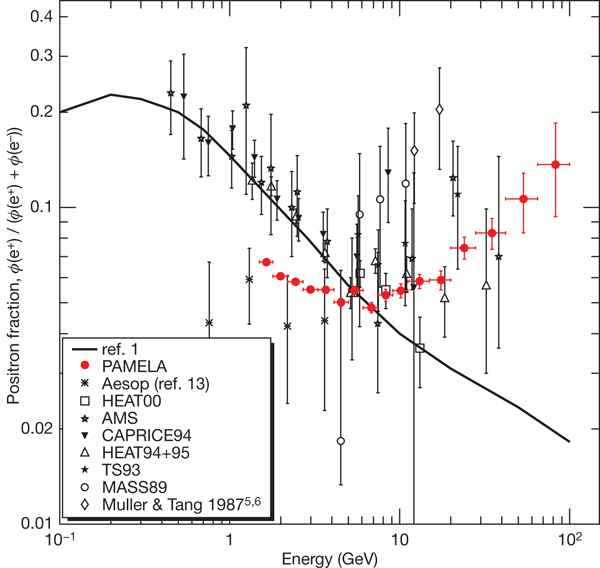
\includegraphics[width=\linewidth]{nature07942-f22jpg.jpeg}
\column{0.65\linewidth}
\begin{itemize}
\item Pamela discovered a source of high-energy positrons in primary cosmic rays (2008)
\begin{itemize}
\item could be undiscovered nearby pulsars
\item could be WIMP-WIMP annihilation
\end{itemize}

\item If it's WIMP-WIMP annihilation, the observed cross-section is too large for the ``WIMP miracle'' scenario
\end{itemize}
\end{columns}

\begin{columns}
\column{0.65\linewidth}
\begin{itemize}
\item Introducing a long-range force in the dark matter sector,
  mediated by ``$a$'' (new boson; $m_a \sim 1$~GeV/$c^2$), enhances
  annihilation cross-section in the present universe (when WIMPs have
  low velocity)
\item $m_a \sim 1$~GeV/$c^2$ also explains lack of excess in antiprotons: \mbox{kinematically forbidden\hspace{1.5 cm}\href{http://arxiv.org/abs/0810.0713}{\textcolor{blue}{hep-ph/0810.0713}}\hspace{-9 cm}}
\end{itemize}

\column{0.35\linewidth}
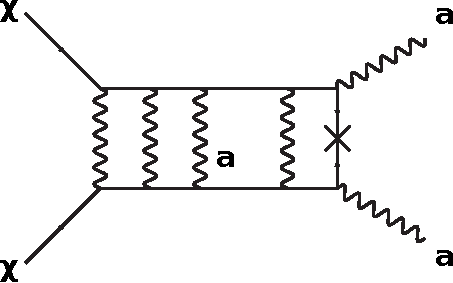
\includegraphics[width=\linewidth]{sommerfeld.pdf}
\end{columns}
\end{frame}

\begin{frame}
\frametitle{Very quick motivation (2/2)}

\begin{columns}
\column{0.32\linewidth}
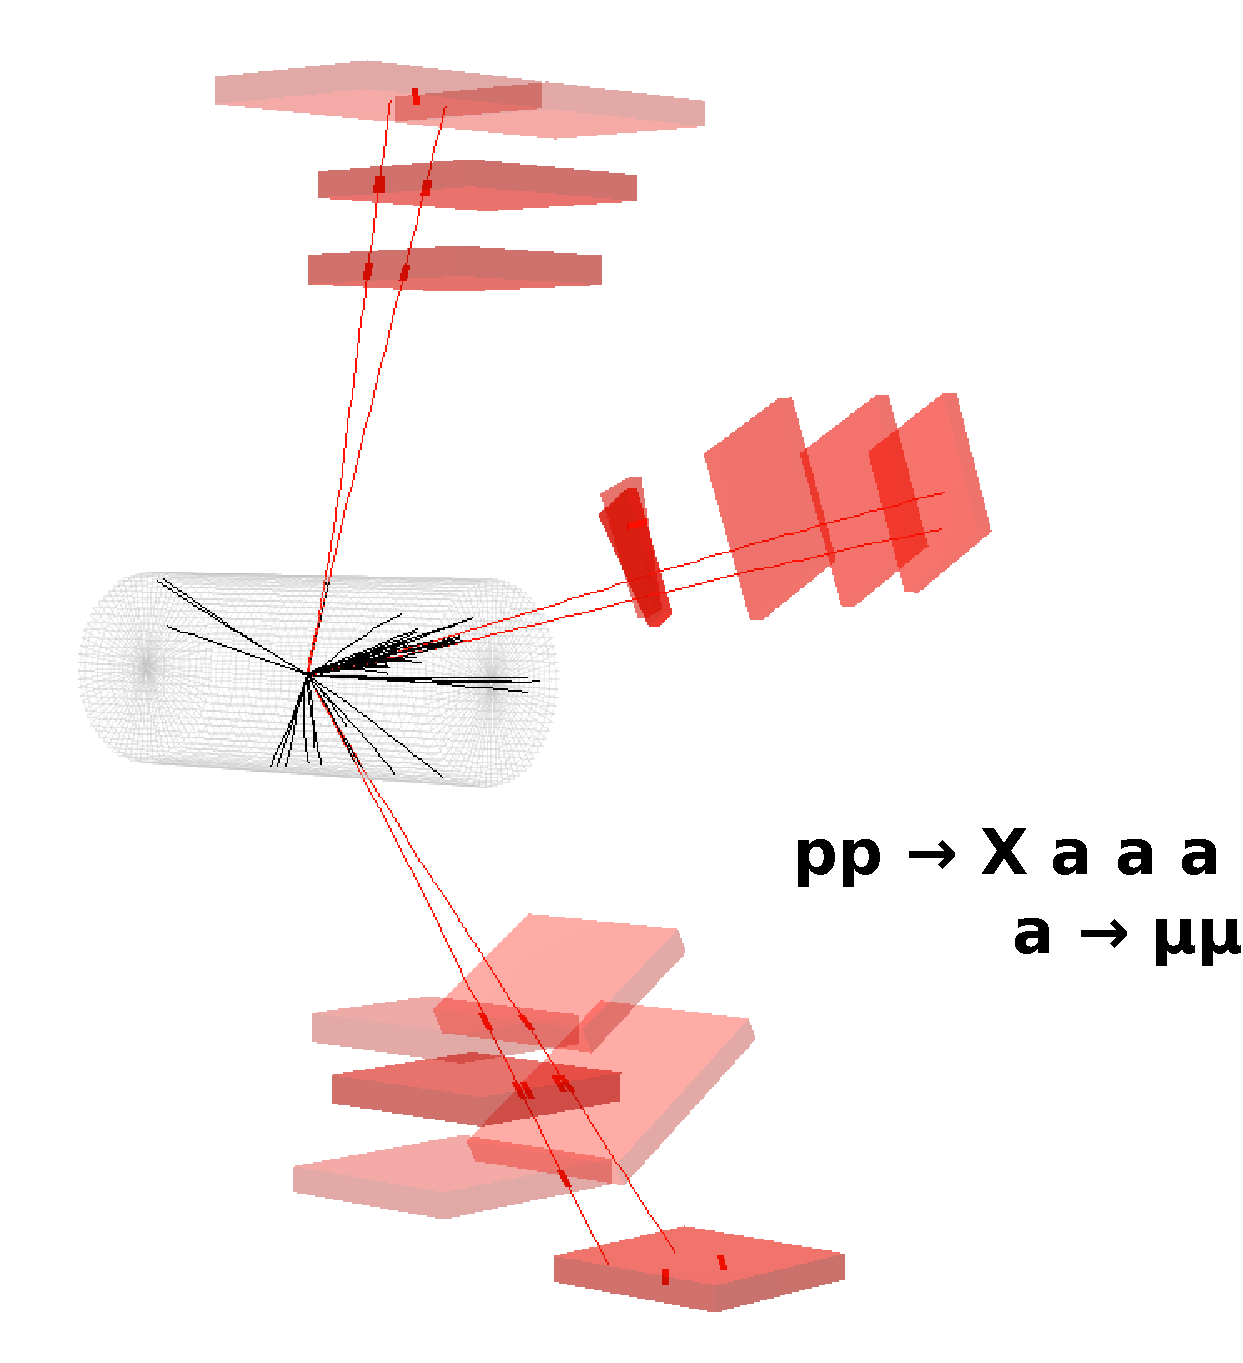
\includegraphics[width=\linewidth]{eventdisplay_3d.pdf}

\vspace{0.5 cm}
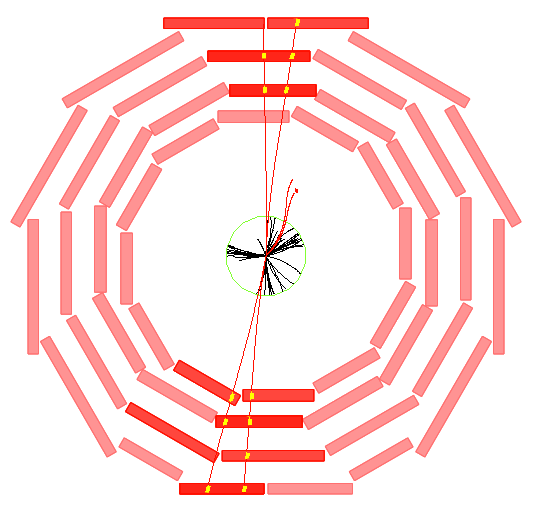
\includegraphics[width=\linewidth]{eventdisplay_rphi.png}

\column{0.68\linewidth}
\begin{itemize}
\item Not a specific model, but a general theoretical idea (``Lepton Jets'')
\begin{itemize}
\item many different scenarios proposed
\item other properties of $a$ are not restricted
\item there may be several $a_i$ with different masses, leading to cascades
\end{itemize}
\item Need to be able to reconstruct the general signature of ``collimated leptons,'' or low-mass, high-$\vec{p}$ groups of leptons (muons)
\end{itemize}

\vspace{-0.4 cm}
\begin{center}
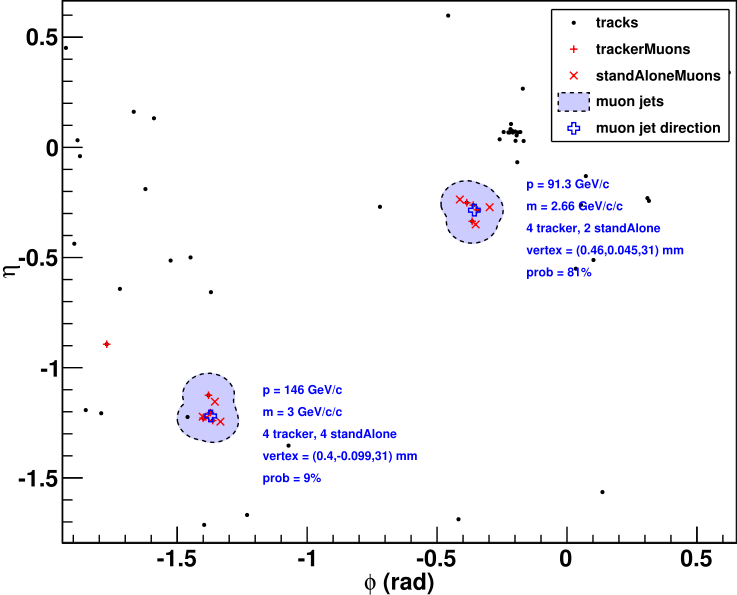
\includegraphics[width=0.65\linewidth]{example_event_display_3.png}
\end{center}
\end{columns}
\end{frame}

\begin{frame}
\frametitle{``Lepton Jets'' at CMS}
\framesubtitle{\href{https://twiki.cern.ch/twiki//bin/viewauth/CMS/ExoticaMuonJets}{\textcolor{blue}{https://twiki.cern.ch/twiki//bin/viewauth/CMS/ExoticaMuonJets}}}

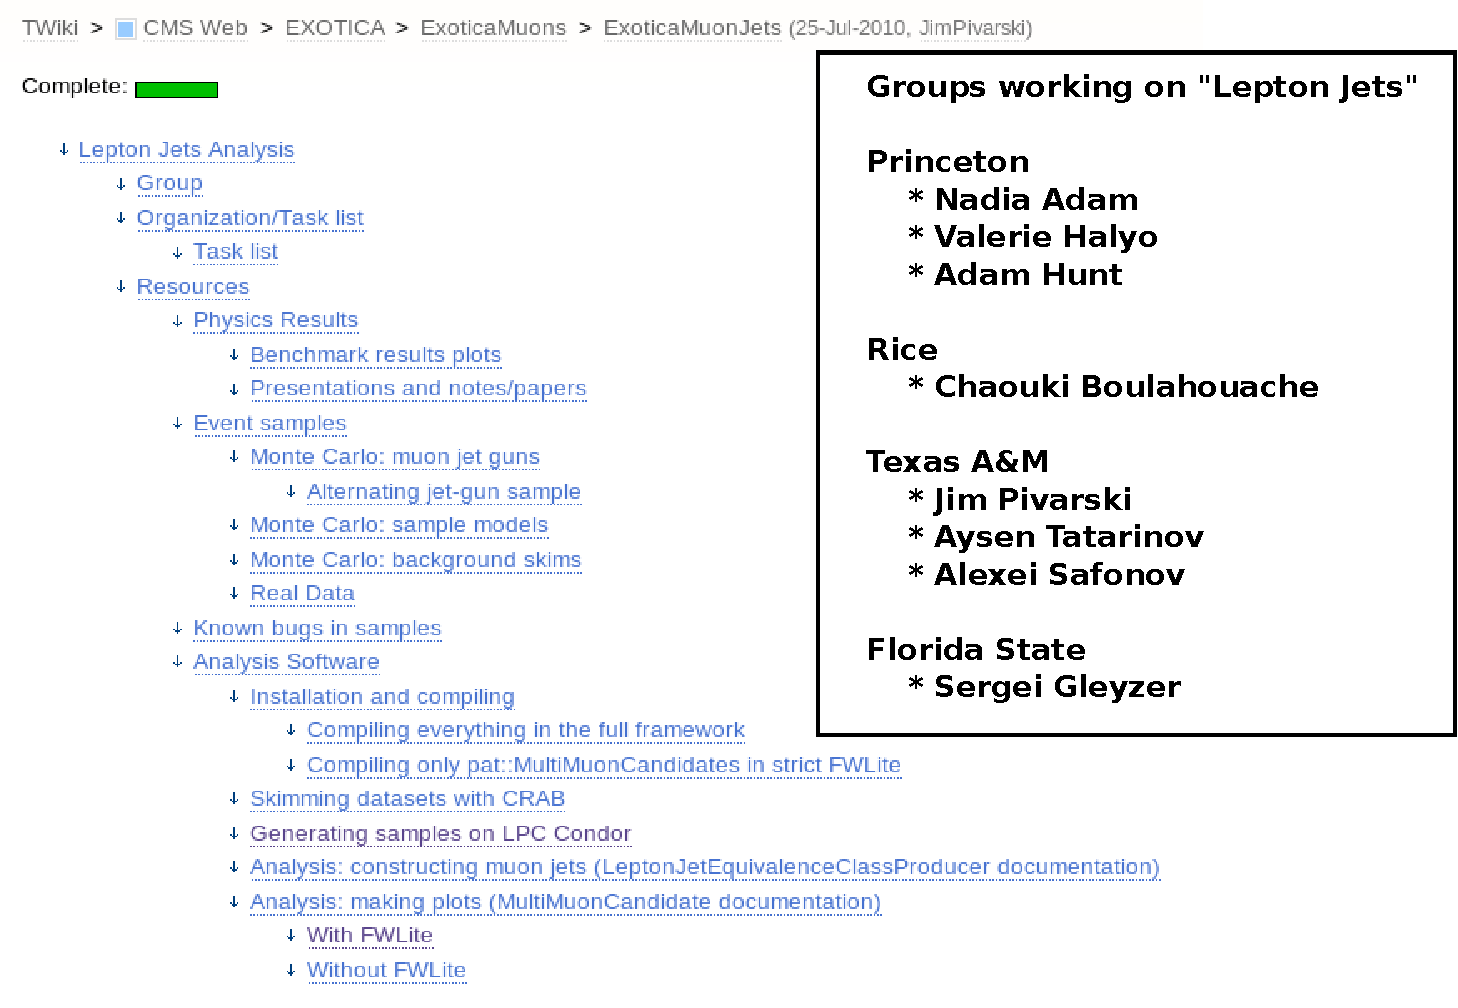
\includegraphics[width=\linewidth]{twiki.pdf}

But this talk will only be on the A\&M work; more later\ldots
\end{frame}

\begin{frame}
\frametitle{Method and infrastructure}
\begin{itemize}
\item Develop a ``$\mu$-group'' object, like any other object in CMS
\begin{itemize}
\item study its performance
\item use it in searches
\end{itemize}

\item Software model:

\mbox{ } \hfill 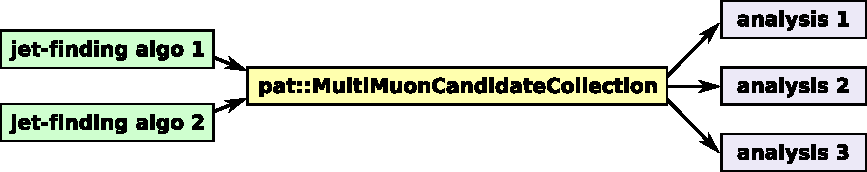
\includegraphics[width=0.8\linewidth]{jets_to_analyses.pdf} \hfill \mbox{ }

\begin{itemize}
\item \textcolor{darkblue}{pat::MultiMuonCandidate} is a persistent group of $N$ muons with methods to perform vertexing and specialized isolation (neighboring muons must not cancel each other out!)
\item \textcolor{darkblue}{LeptonJetsEquivalenceClassProducer} groups muons according to their ``closeness'' (next page)
\item \textcolor{darkblue}{MultiParticleByMassGunProducer} simulates pairs and quadruplets of muons uniformly in mass-momentum space
\end{itemize}

\item SVN repository: \href{https//svnweb.cern.ch/cern/wsvn/LeJOG/trunk/}{\textcolor{blue}{https//svnweb.cern.ch/cern/wsvn/LeJOG/trunk/}}
\end{itemize}
\end{frame}

\begin{frame}
\frametitle{Merging muons into groups}

\vspace{0.5 cm}
\begin{columns}
\column{0.5\linewidth}
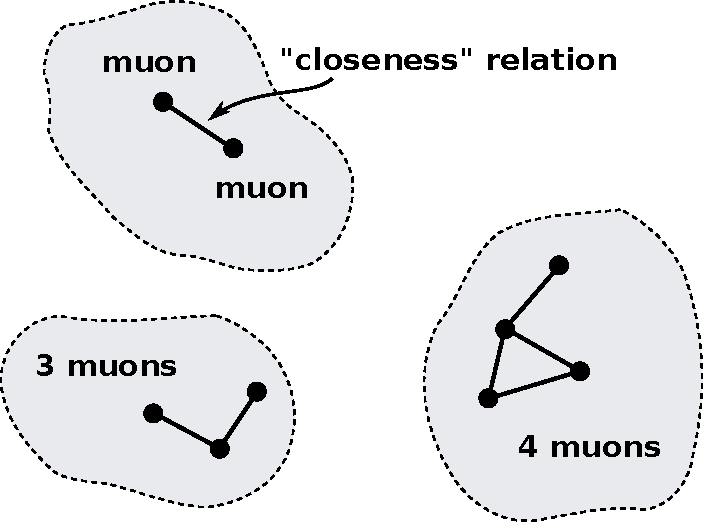
\includegraphics[width=\linewidth]{closeness.pdf}
\column{0.5\linewidth}
Muons are grouped if
\begin{itemize}
\item they are ``close'' to each other
\item they're close to another muon which is close to another, etc.
\end{itemize}

No dependence on the order of the grouping process, easy to analyze
\end{columns}

\begin{itemize}
\item Definition of ``closeness'' is tunable, with these ingredients:
\begin{itemize}\setlength{\itemsep}{0.1 cm}
\item $\Delta R$: geometrically close in a metric with uniform background
\item $m_\s{inv}$: guarantees that low-mass objects will be found, regardless of boost
\item $P_\s{vertex}$: requires a consistent track vertex
\item opposite charge: avoids connecting groups that can't be from the same neutral resonance
\end{itemize}
\end{itemize}
\end{frame}

\begin{frame}
\frametitle{Merging muons into groups}

Grouping efficiency vs.\ reconstructed mass and $\Delta R$

{\scriptsize (denominator: reconstructed two muons; numerator: grouped them)}

\vfill
\begin{columns}
\column{0.7\linewidth}
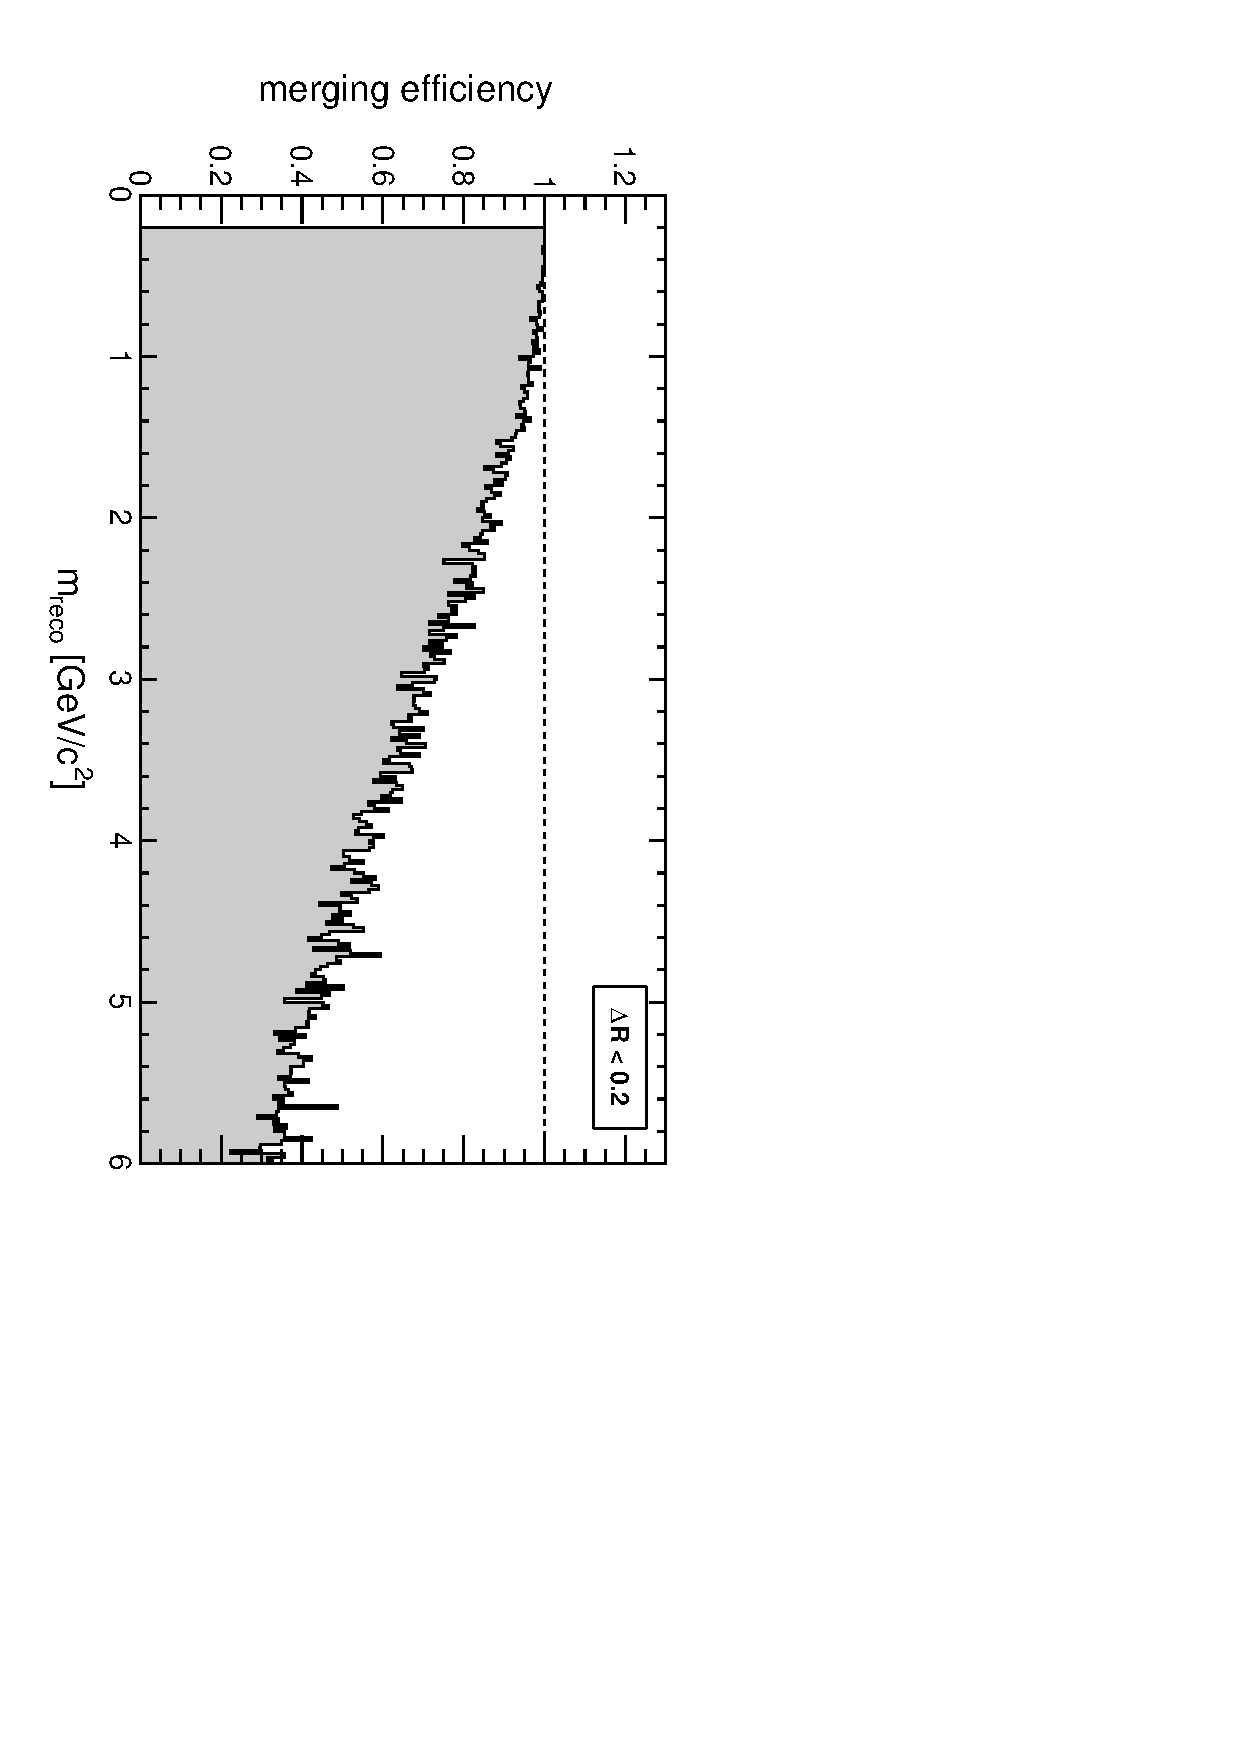
\includegraphics[height=0.5\linewidth, angle=90]{mergingeff_recomass_GroupByDeltaR.pdf}
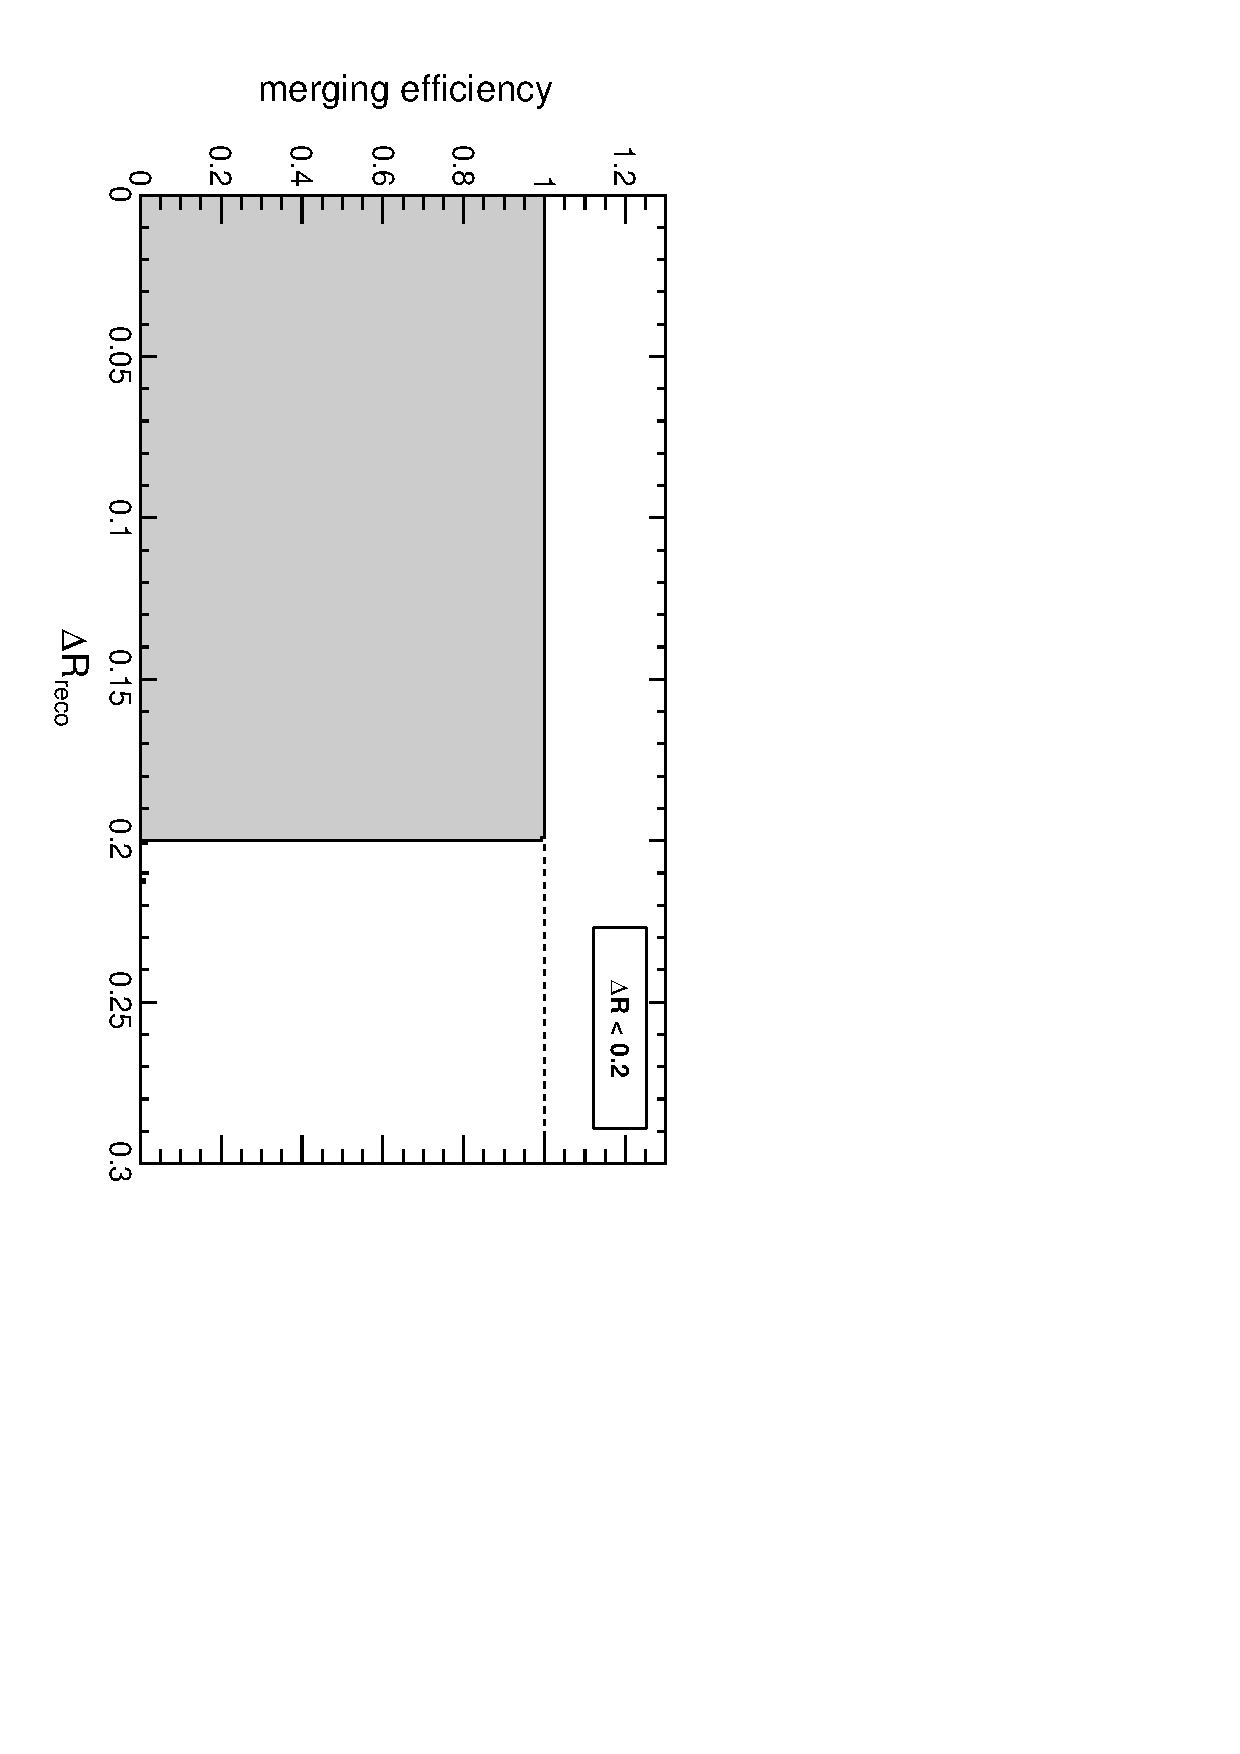
\includegraphics[height=0.5\linewidth, angle=90]{mergingeff_recodr_GroupByDeltaR.pdf}
\column{0.3\linewidth}
$\Delta R < 0.2$
\end{columns}

\begin{columns}
\column{0.7\linewidth}
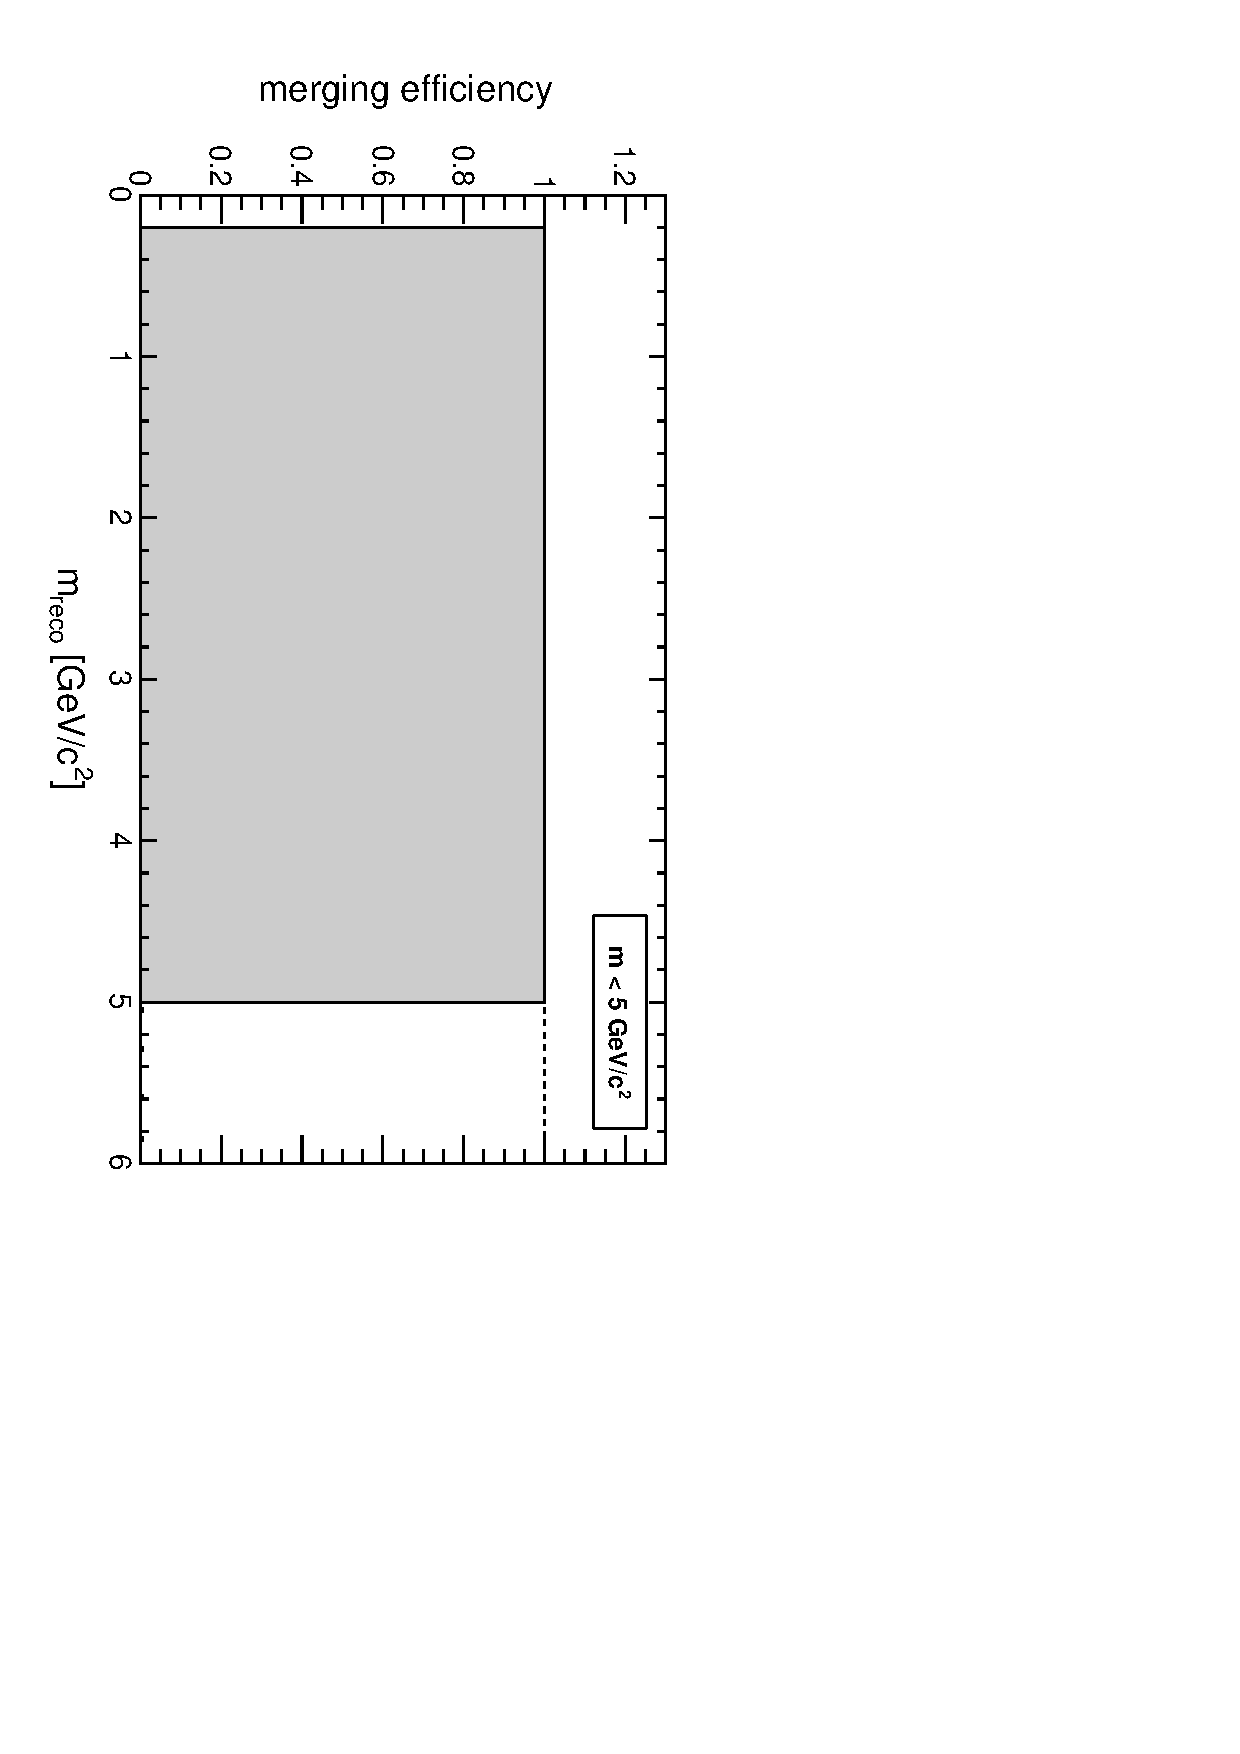
\includegraphics[height=0.5\linewidth, angle=90]{mergingeff_recomass_GroupByMass.pdf}
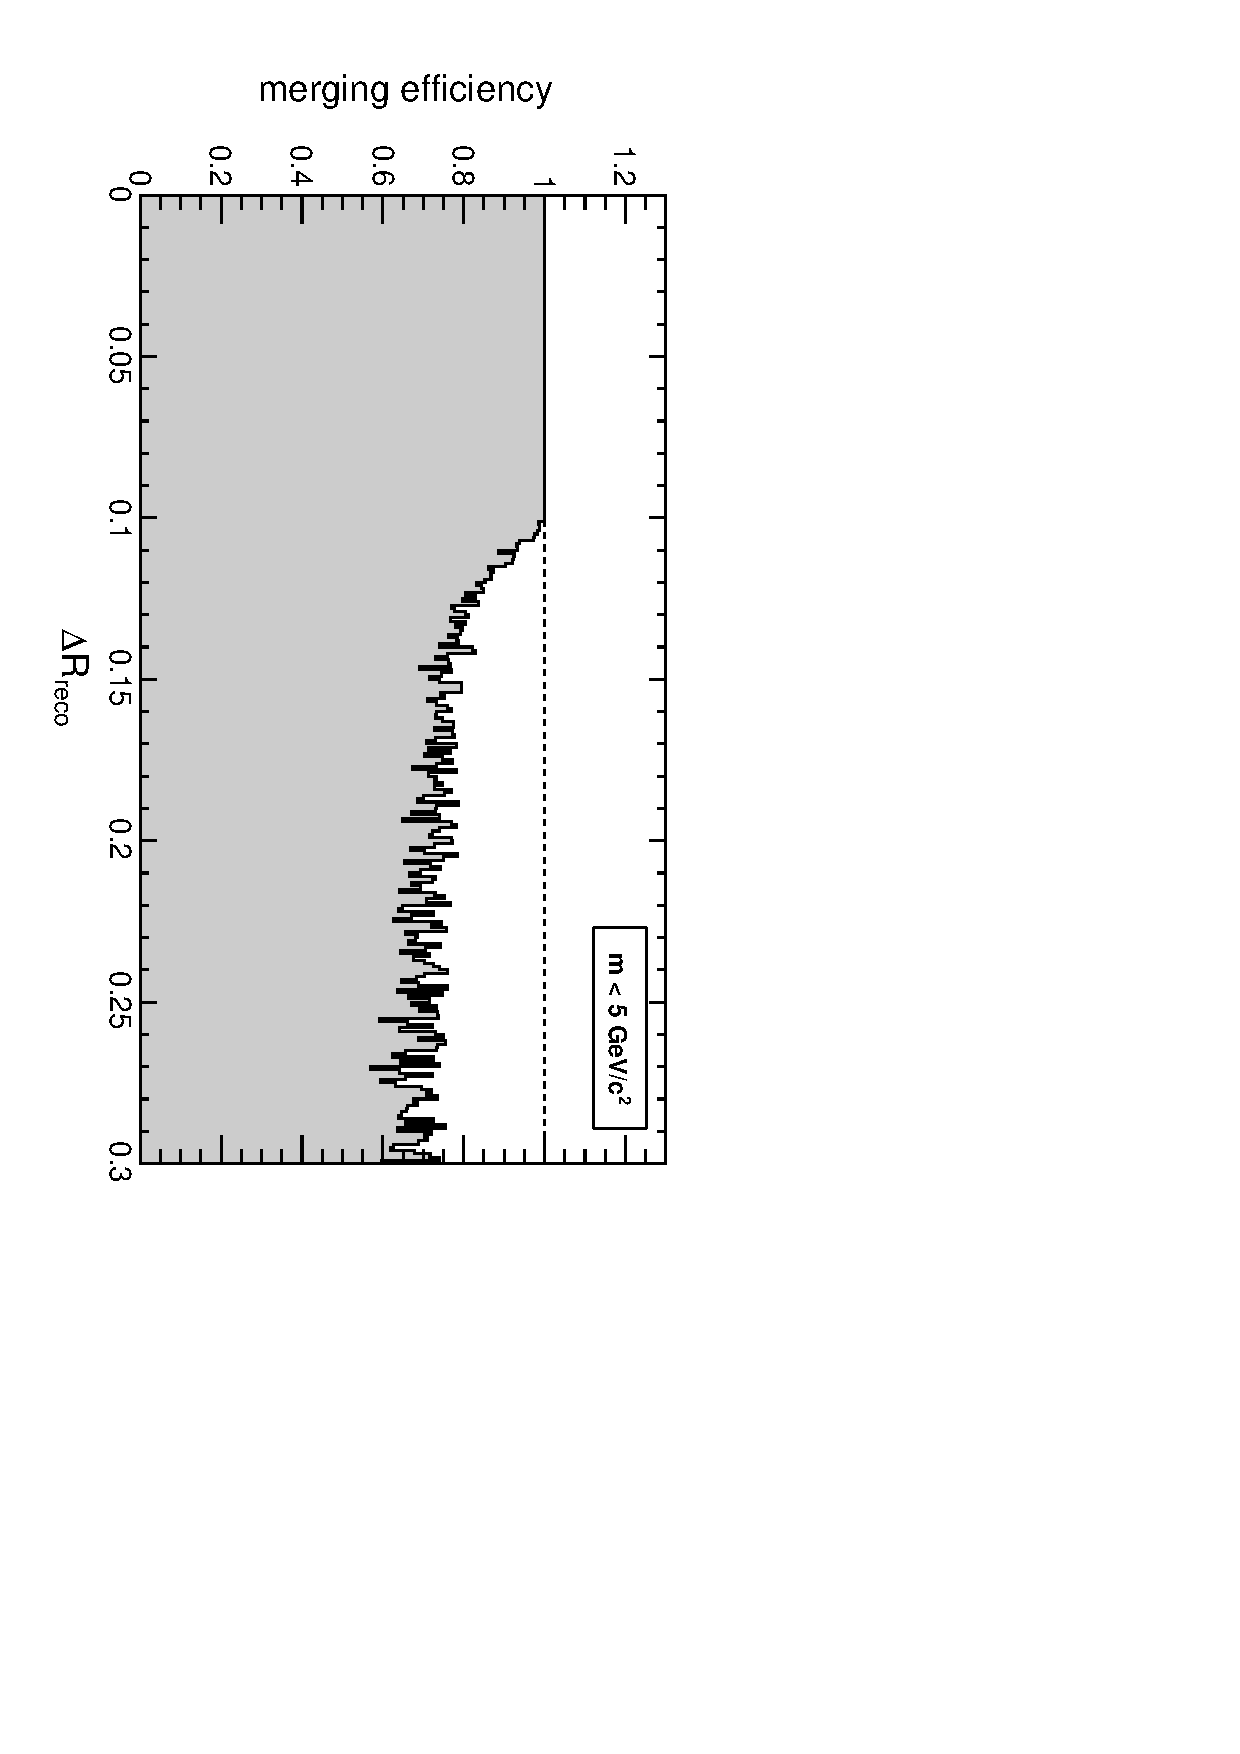
\includegraphics[height=0.5\linewidth, angle=90]{mergingeff_recodr_GroupByMass.pdf}
\column{0.3\linewidth}
$m_\s{inv} < 5$~GeV/$c$
\end{columns}

\begin{columns}
\column{0.7\linewidth}
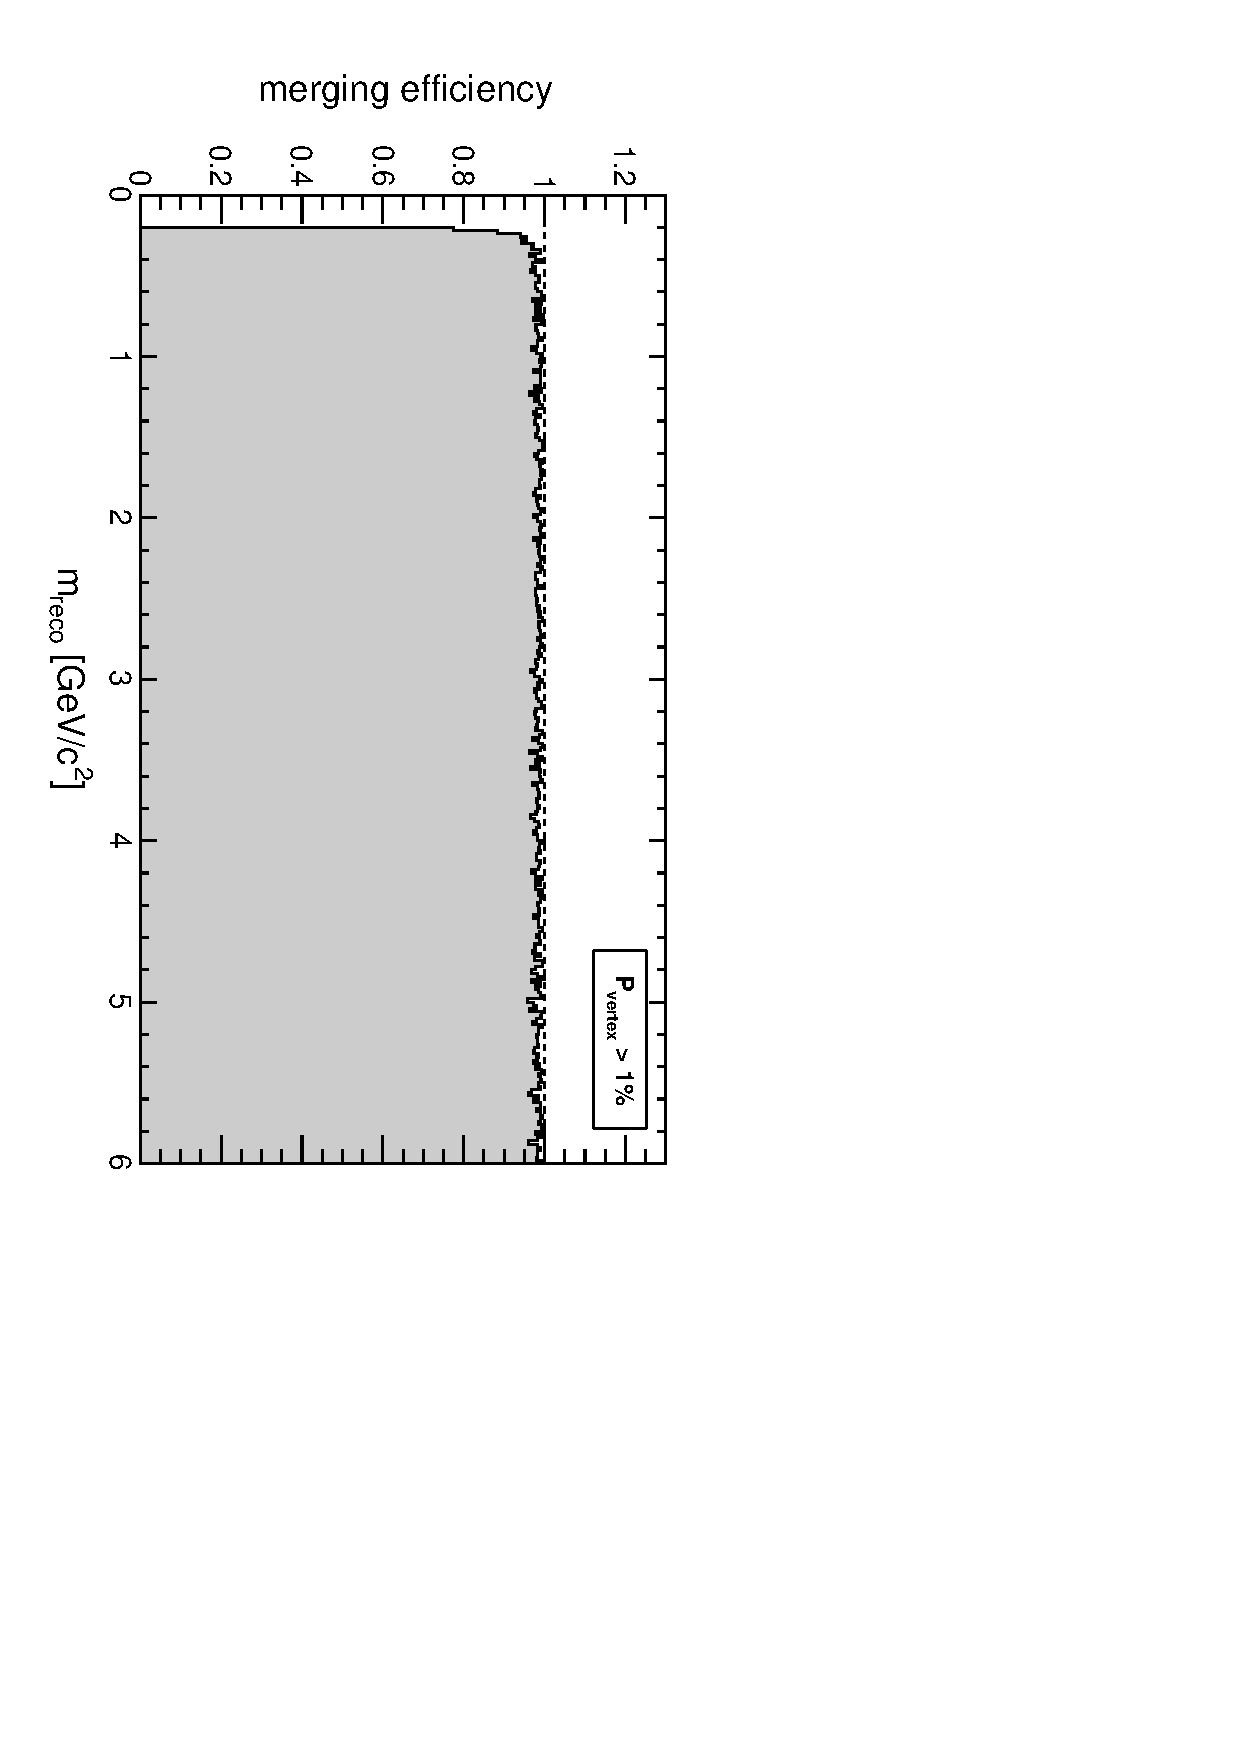
\includegraphics[height=0.5\linewidth, angle=90]{mergingeff_recomass_GroupByVertexProb.pdf}
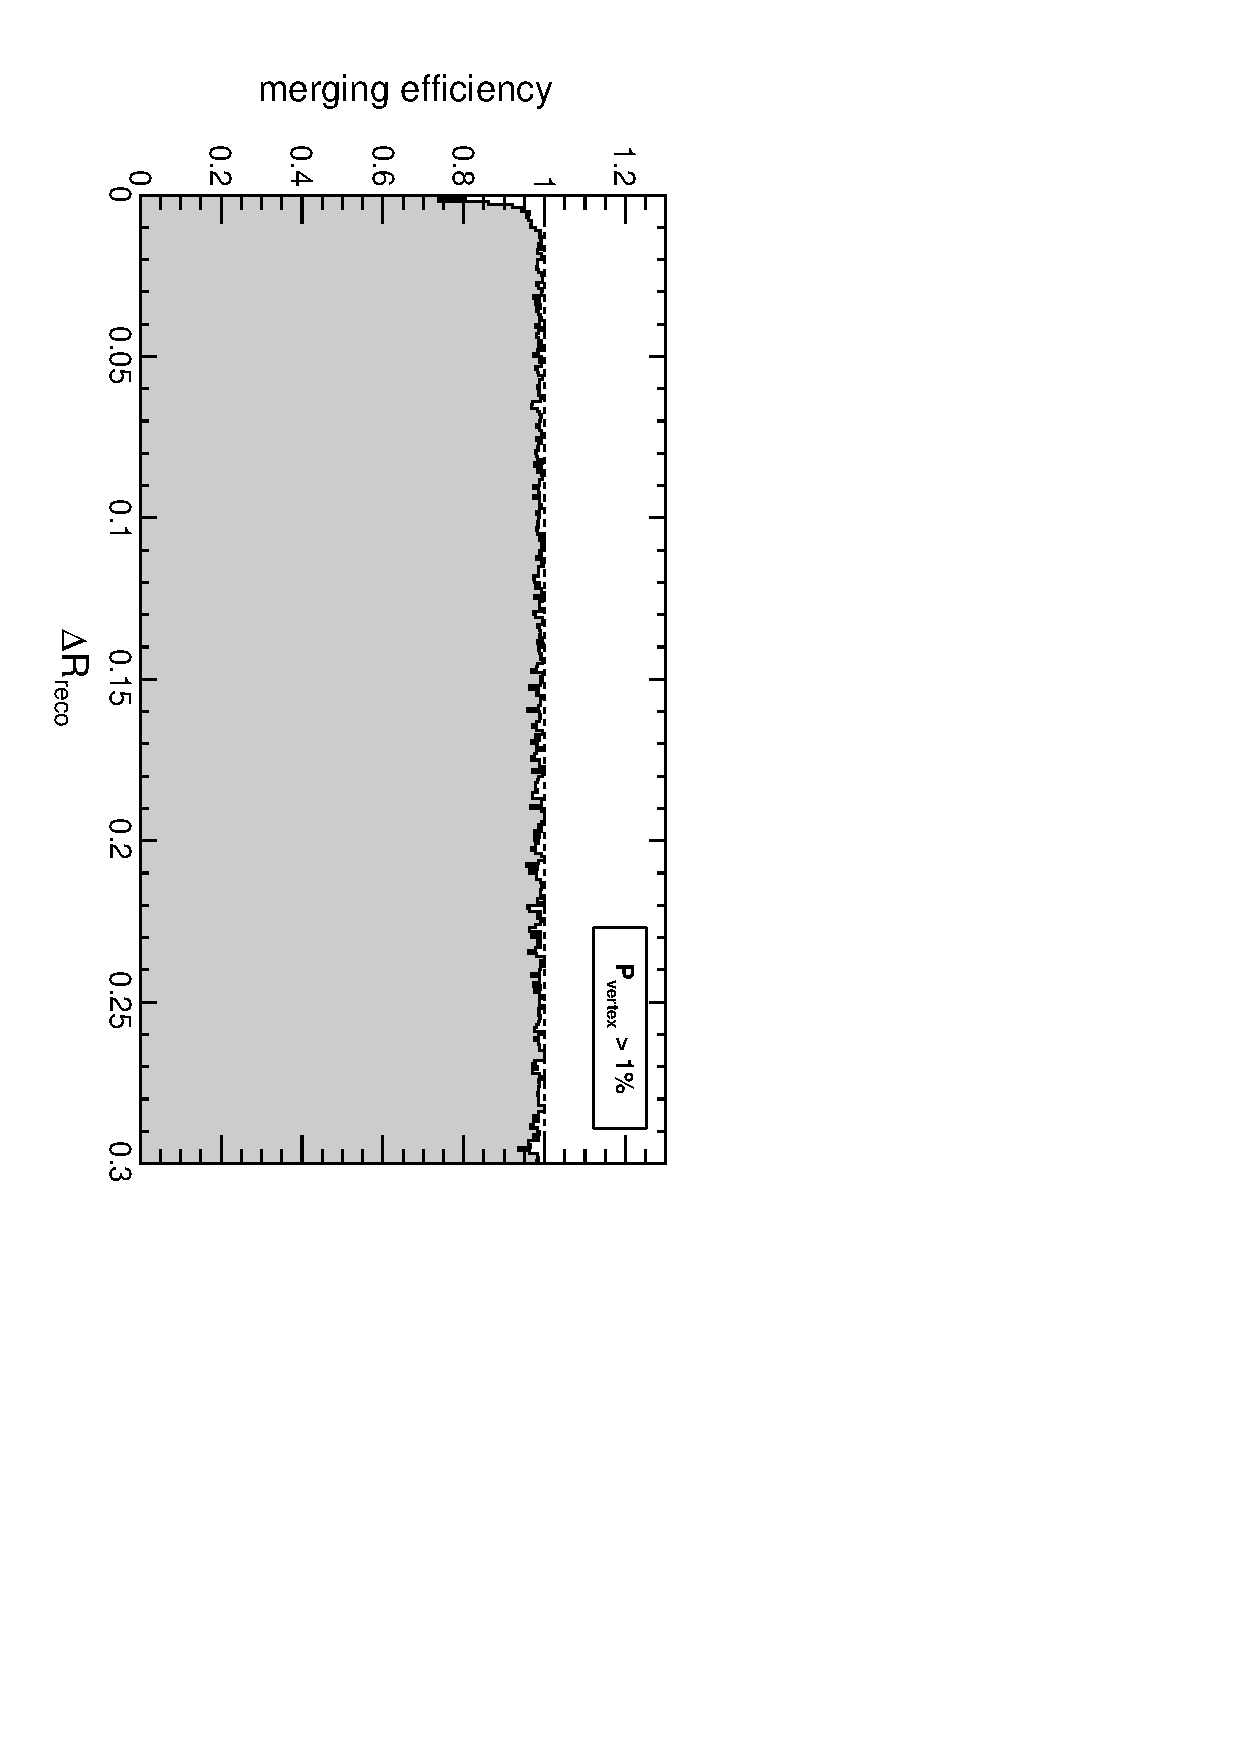
\includegraphics[height=0.5\linewidth, angle=90]{mergingeff_recodr_GroupByVertexProb.pdf}

\column{0.3\linewidth}
$P_\s{vertex} > 1$\%

\vspace{0.25 cm}
{\scriptsize (Note low efficiency due to vertexing failures for collinear muons)}
\end{columns}
\end{frame}

\begin{frame}
\frametitle{Merging muons into groups}
Optimization: group by
\begin{center}
$(m_{\mbox{\scriptsize inv}} < 5\mbox{ GeV/}c \mbox{\bf\mbox{ and }} P_{\mbox{\scriptsize vertex}} > 1\%) \mbox{\bf\mbox{ or }} \Delta R < 0.1$
\end{center}
\begin{itemize}
\item We guarantee that we get low-mass objects
\item Usually require them to vertex well
\item Except when they're very close together
\end{itemize}

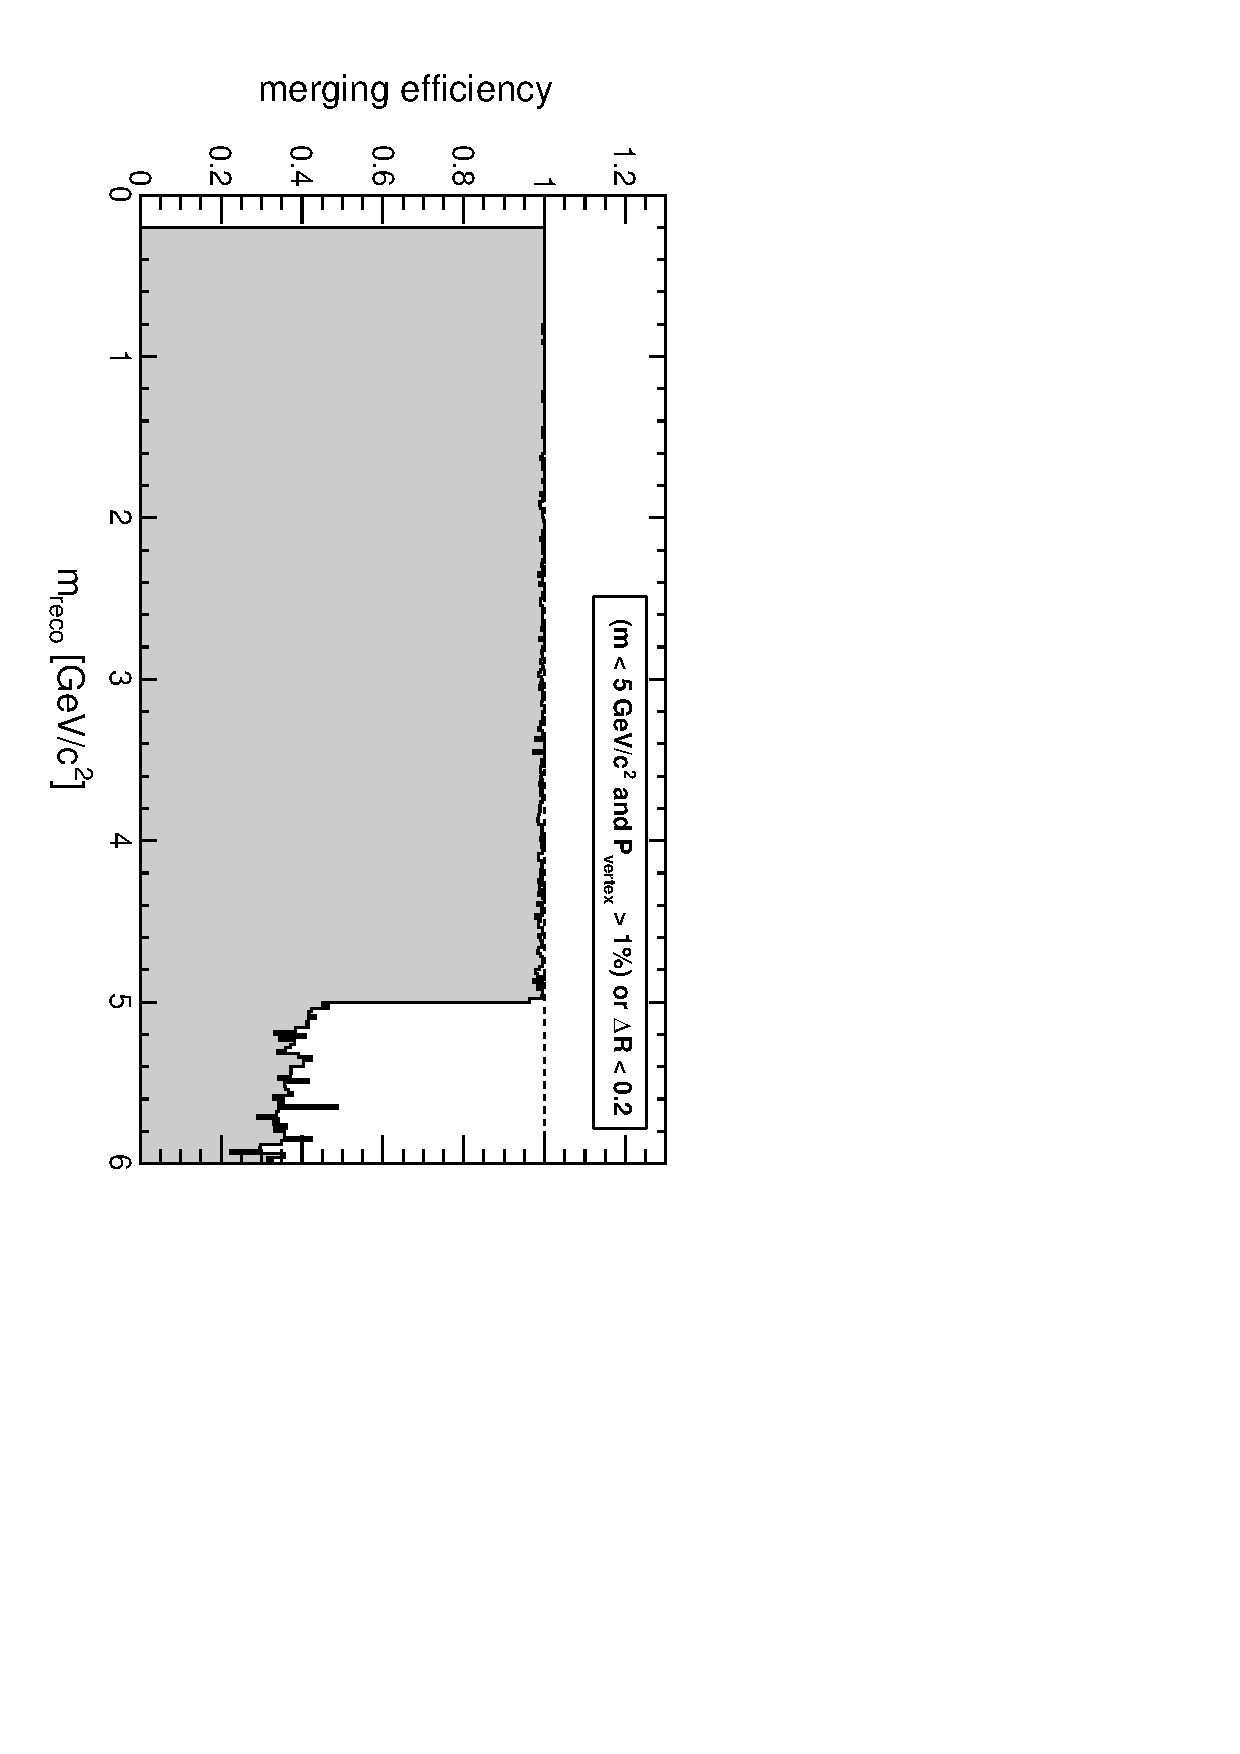
\includegraphics[height=0.5\linewidth, angle=90]{mergingeff_recomass_GroupByMassAndVertexProbOrDeltaR.pdf}
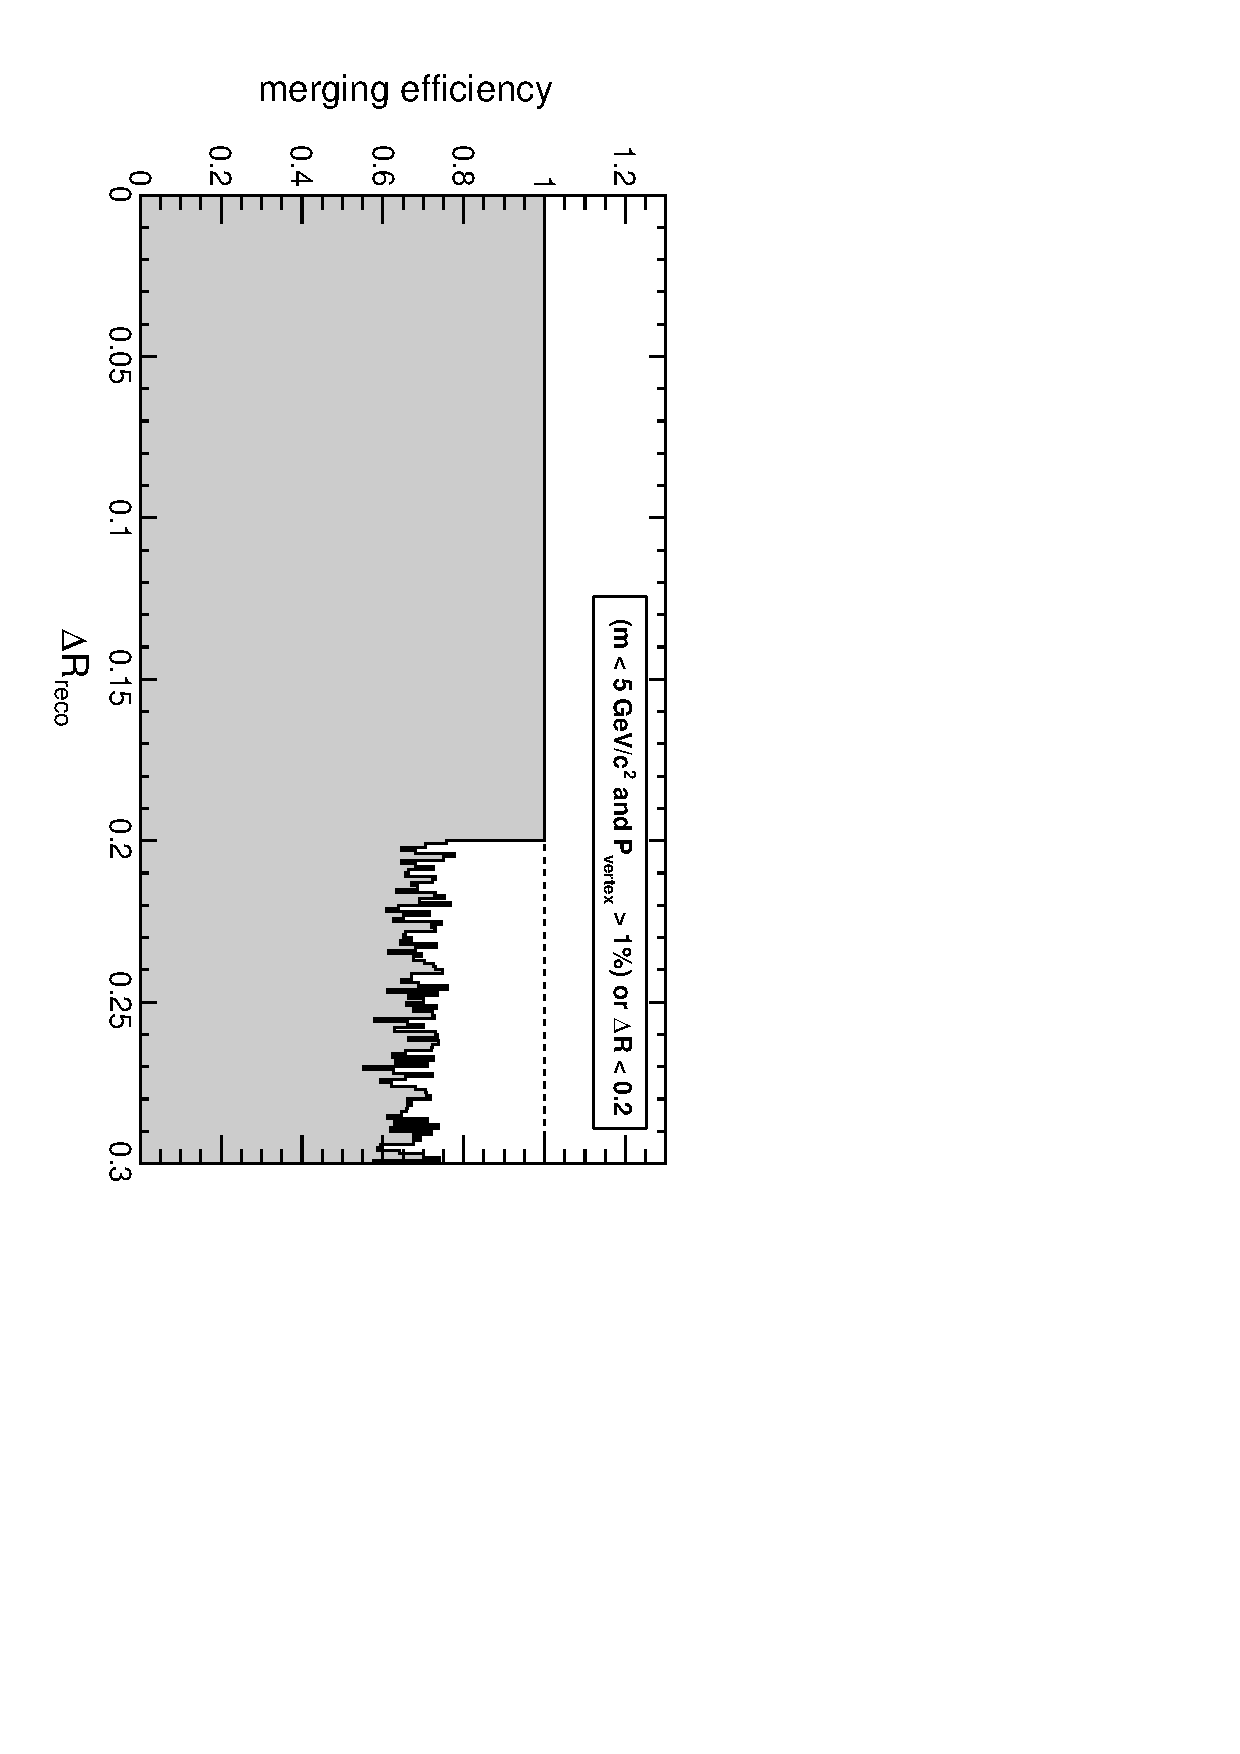
\includegraphics[height=0.5\linewidth, angle=90]{mergingeff_recodr_GroupByMassAndVertexProbOrDeltaR.pdf}

\vfill
Leave the opposite-sign requirement for later
\end{frame}

\begin{frame}
\frametitle{Merging muons into groups}

\begin{itemize}
\item If we have two low-mass ($m < 5$~GeV/$c^2$) dimuons in an event,
  what is the probability that they will be merged into two groups or one group? {\scriptsize (denominator: reco'ed four muons; numerator: grouped them)}
\begin{itemize}\setlength{\itemsep}{0.1 cm}
\item $\alpha_\s{pair-pair}$ is the 3D angle between dimuons
\item $m_\s{pair-pair}$ is the parent particle mass
\item ``crossed'' means 1-2, 3-4 gets reconstructed as 1-3, 2-4
\end{itemize}

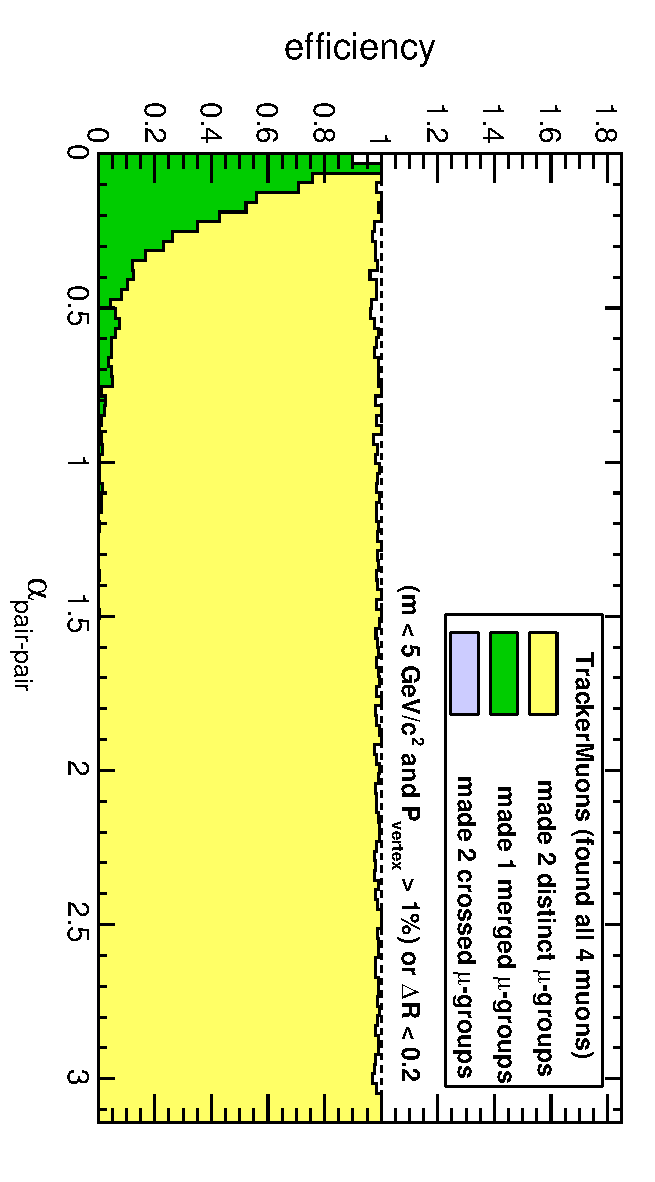
\includegraphics[height=0.5\linewidth, angle=90]{foundopening_TrackerMuonsGroupByMassAndVertexProbOrDeltaR.pdf}
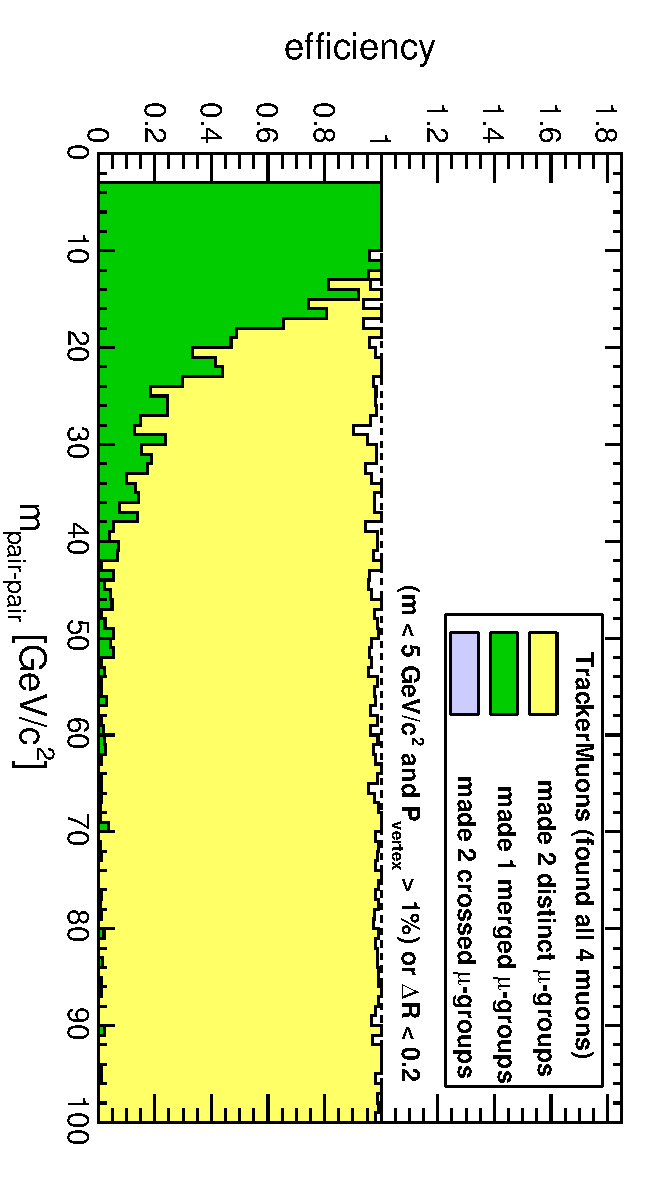
\includegraphics[height=0.5\linewidth, angle=90]{foundmass_TrackerMuonsGroupByMassAndVertexProbOrDeltaR.pdf}

\item Can be tuned with grouping criteria: loose ``closeness''
  criteria yield higher efficiency for pairs and higher probability
  of pair-merging
\item The plots above came from a flat-generated pair-pair gun; should
  try with realistic cascades because it could depend on kinematics
\end{itemize}
\end{frame}

\begin{frame}
\frametitle{Extra muons in group}

\begin{itemize}
\item $\mu$-groups can absorb an extra muon from unrelated \mbox{tracks in the event\hspace{-1 cm}}
\item Below: simulations with increasing amounts of pile-up ($\frac{N_\s{extra}}{N_\s{total}}$ vs.\ $\eta$)

left: TrackerMuon-groups, right: GlobalMuon-groups
\end{itemize}

\begin{columns}
\column{0.7\linewidth}
\mbox{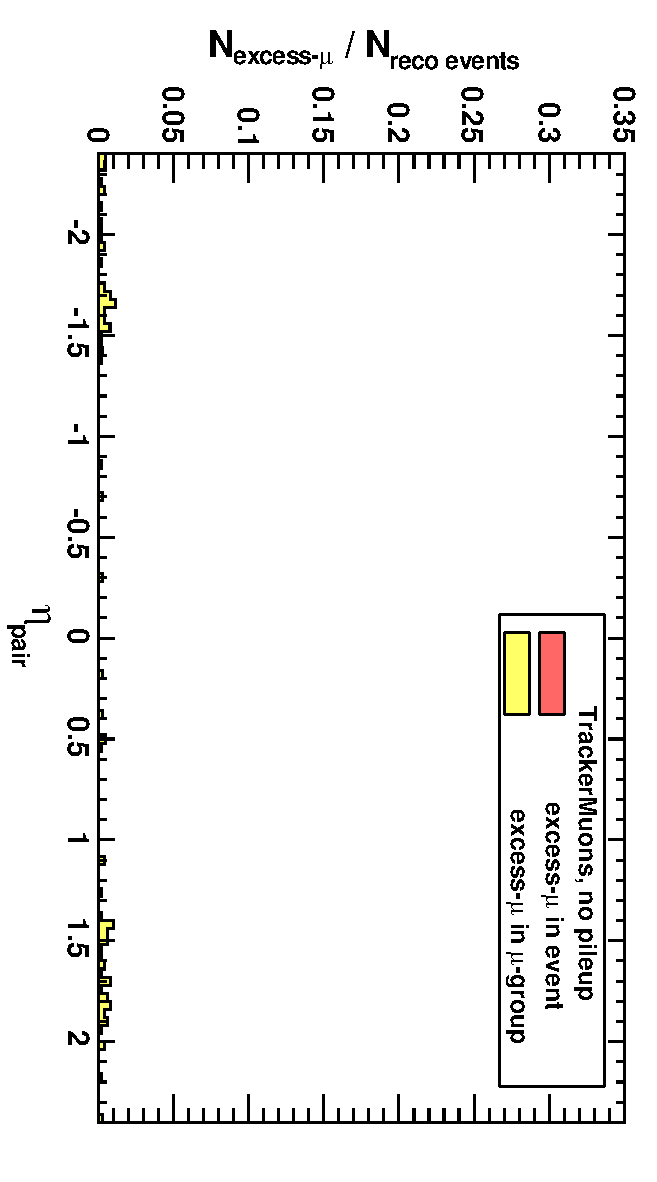
\includegraphics[height=0.5\linewidth, angle=90]{toomanymuons_TrackerMuonsGroupByMassAndVertexProbOrDeltaR.pdf}
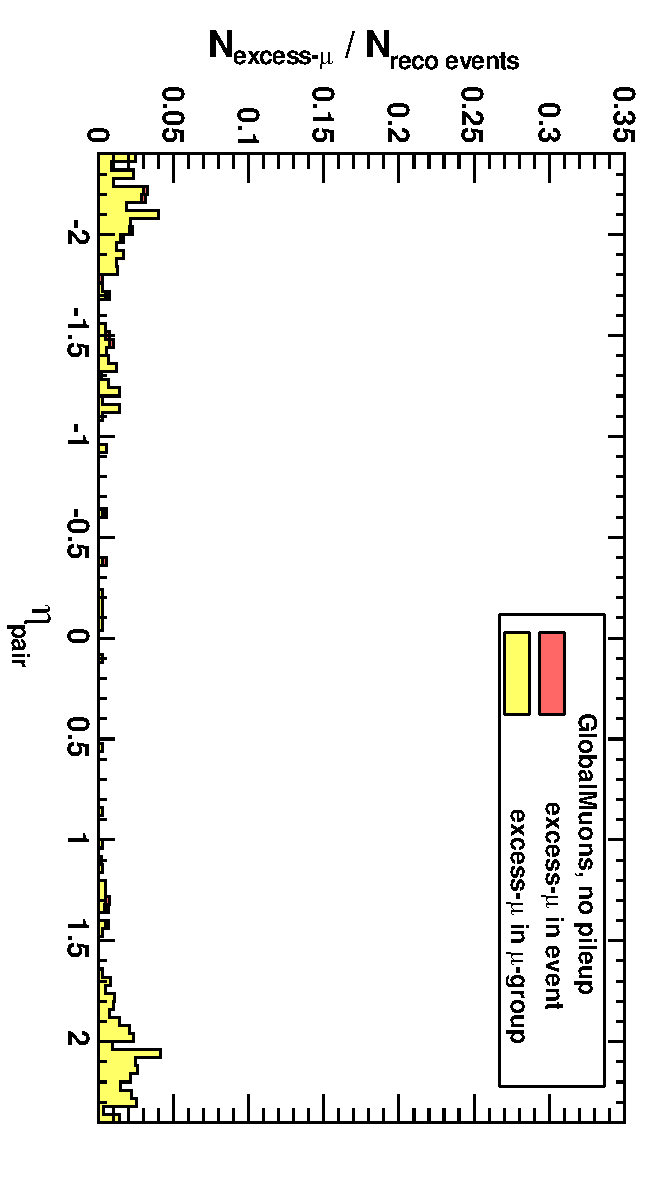
\includegraphics[height=0.5\linewidth, angle=90]{toomanymuons_GlobalMuonsGroupByMassAndVertexProbOrDeltaR.pdf}}

\mbox{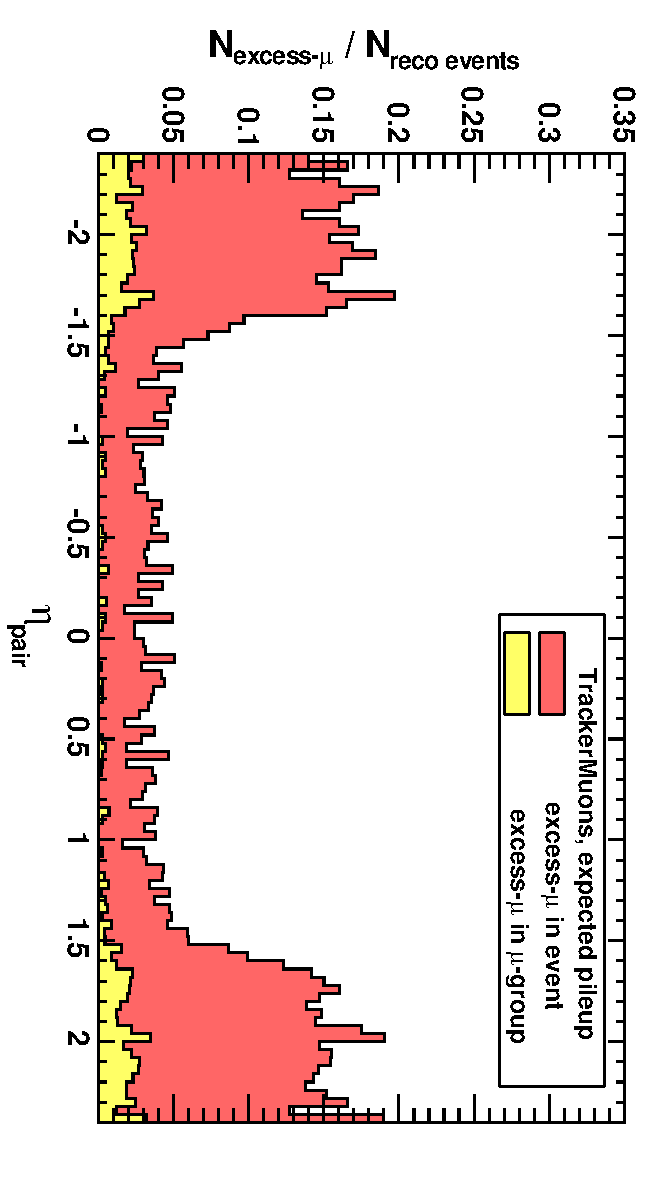
\includegraphics[height=0.5\linewidth, angle=90]{toomanymuons_TrackerMuonsGroupByMassAndVertexProbOrDeltaR_pileup.pdf}
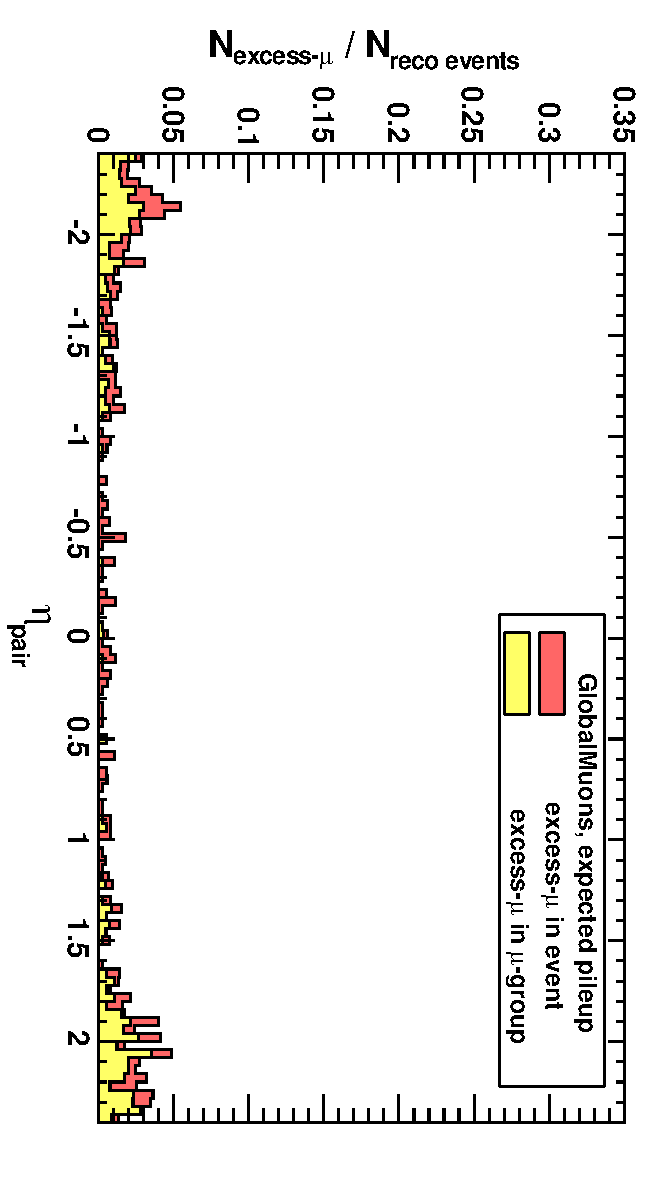
\includegraphics[height=0.5\linewidth, angle=90]{toomanymuons_GlobalMuonsGroupByMassAndVertexProbOrDeltaR_pileup.pdf}}

\mbox{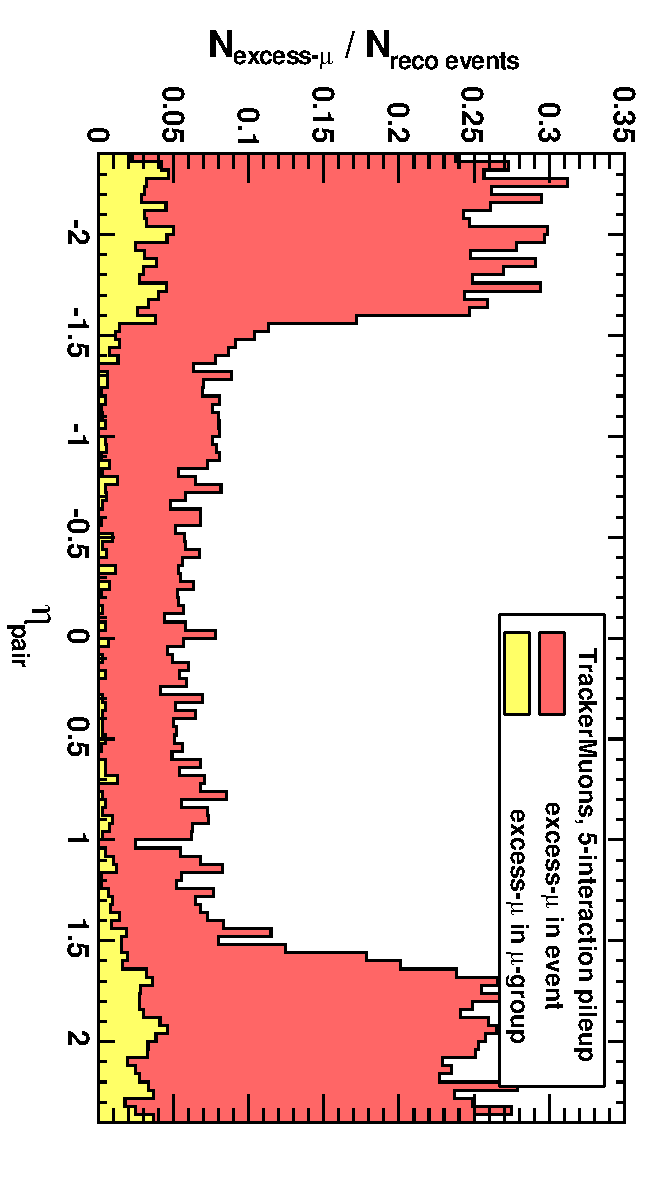
\includegraphics[height=0.5\linewidth, angle=90]{toomanymuons_TrackerMuonsGroupByMassAndVertexProbOrDeltaR_pileup5.pdf}
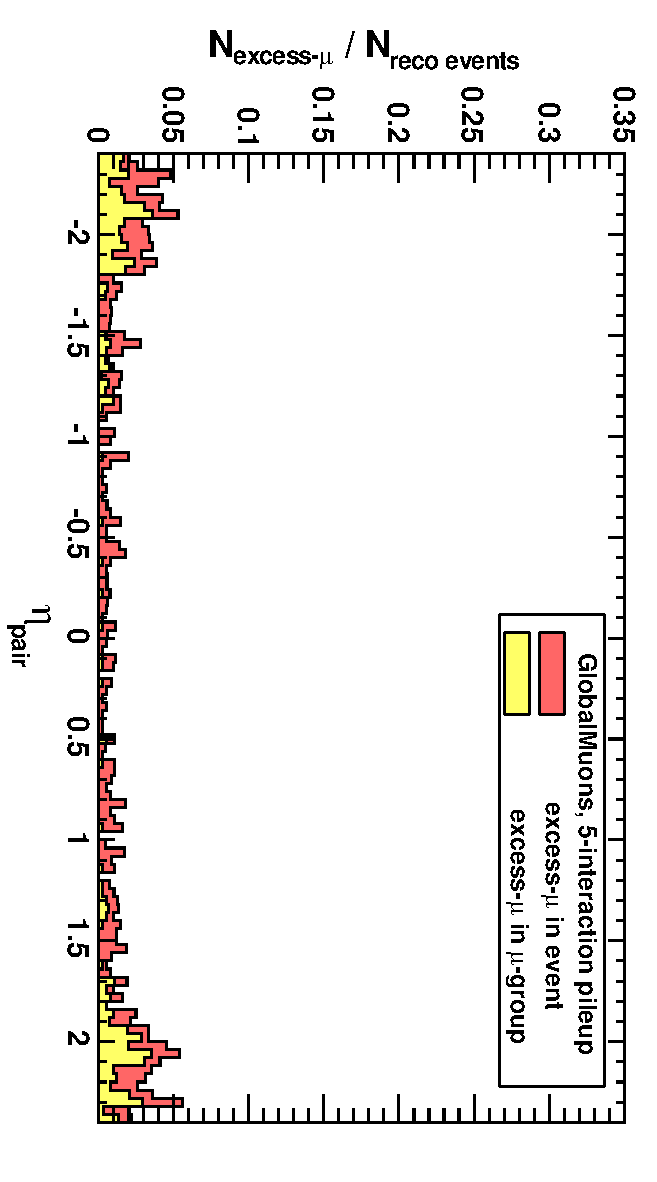
\includegraphics[height=0.5\linewidth, angle=90]{toomanymuons_GlobalMuonsGroupByMassAndVertexProbOrDeltaR_pileup5.pdf}}

\column{0.25\linewidth}
Despite extra tracks identified as muons (red), the extra-muons-in-group (yellow) is controlled by $P_\s{vertex} > 1\%$

\vspace{0.3 cm}
We'll also soon see that fake TrackerMuons can be controlled with quality cuts
\end{columns}
\end{frame}

\begin{frame}
\frametitle{Acceptance and efficiency}
\begin{itemize}
\item Acceptance region of a dimuon defined by $pT_2 > 5$~GeV/$c$ and
  $|\eta_1| < 2.4$ where $pT_2$ is the second-highest $p_T$ muon and
  $\eta_1$ is the highest-$|\eta|$ muon in the event \mbox{\scriptsize (denominator: all; numerator: reco'ed two muons)\hspace{-1 cm}}
\item Try reconstructing muons in four separate \mbox{collections: TrackerMuons,\hspace{-1 cm}}
  StandAloneMuons, StandAlone-SET algorithm, and GlobalMuons

\end{itemize}
\begin{center}
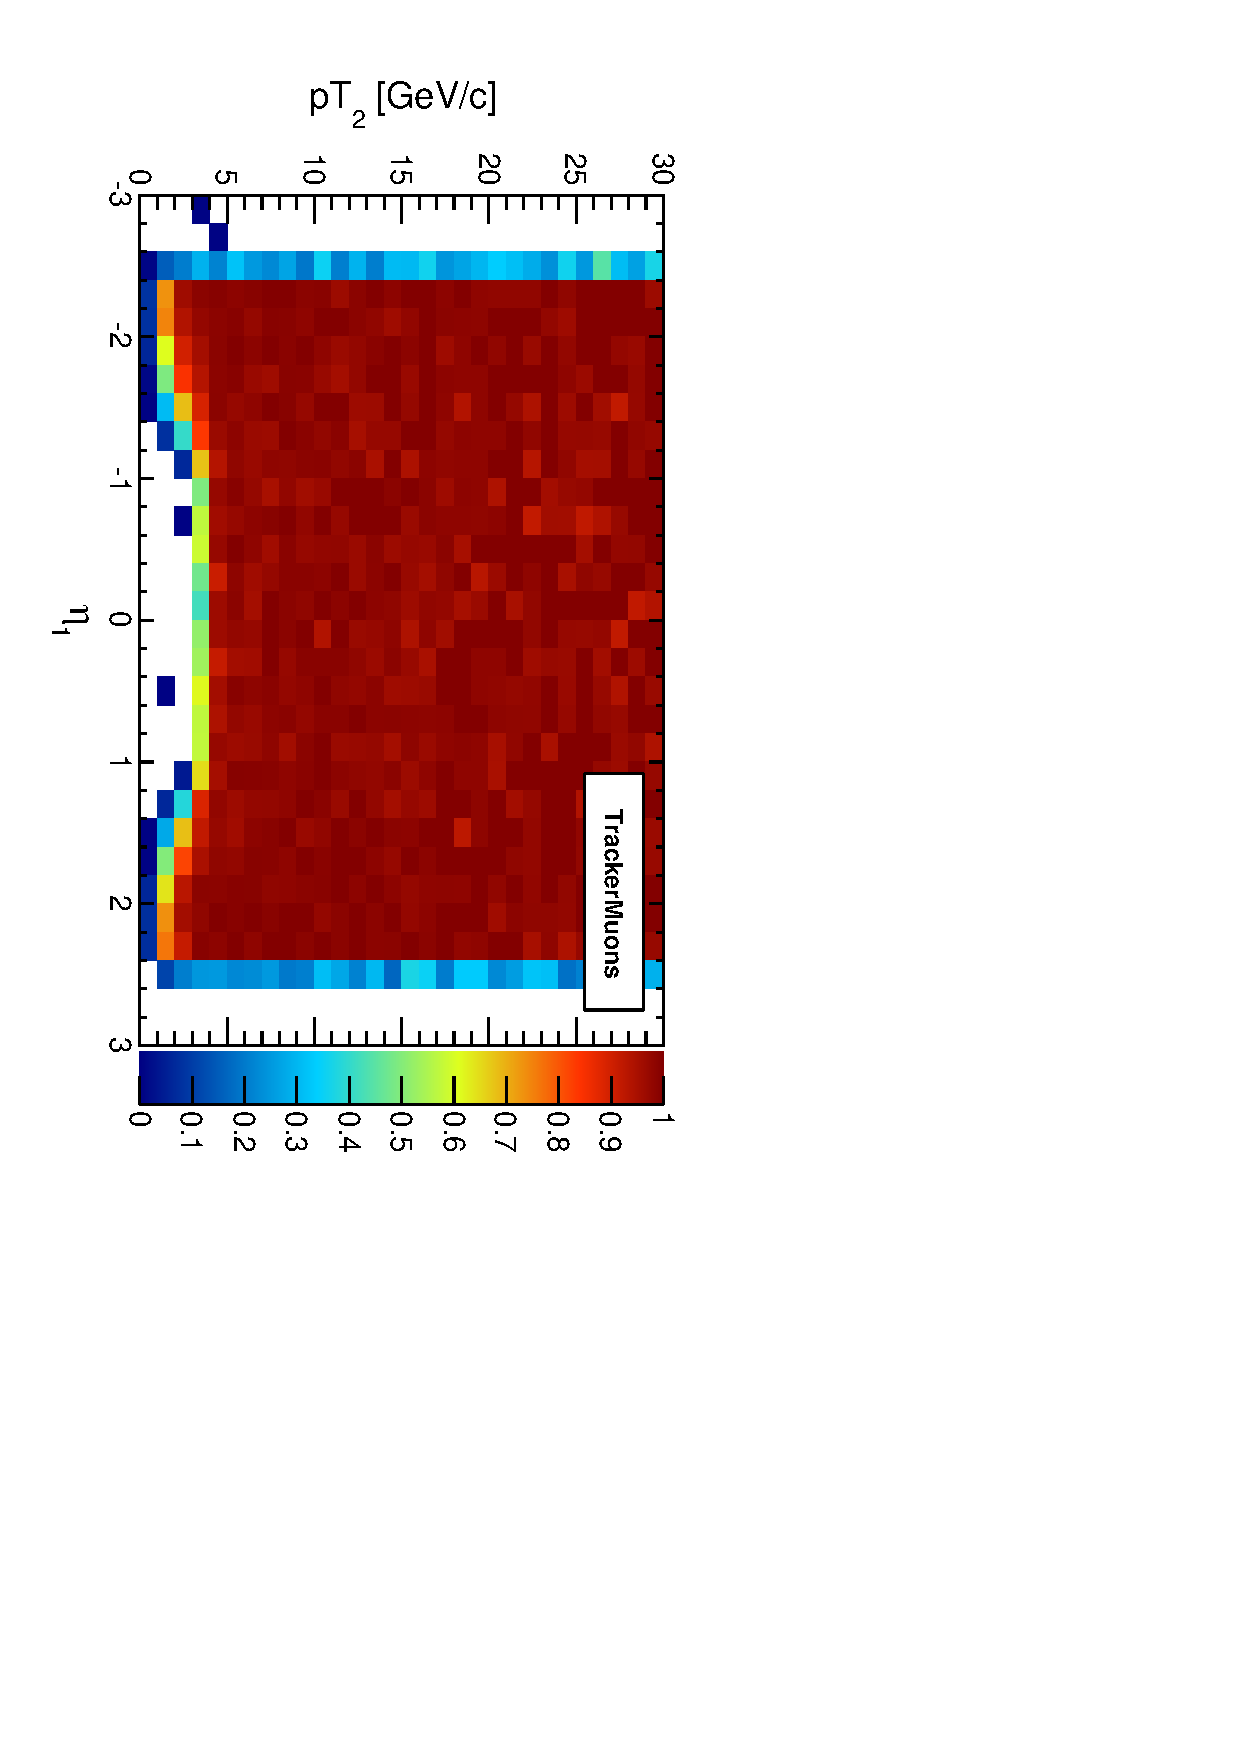
\includegraphics[height=0.45\linewidth, angle=90]{pt2vseta1_TrackerMuons.pdf}
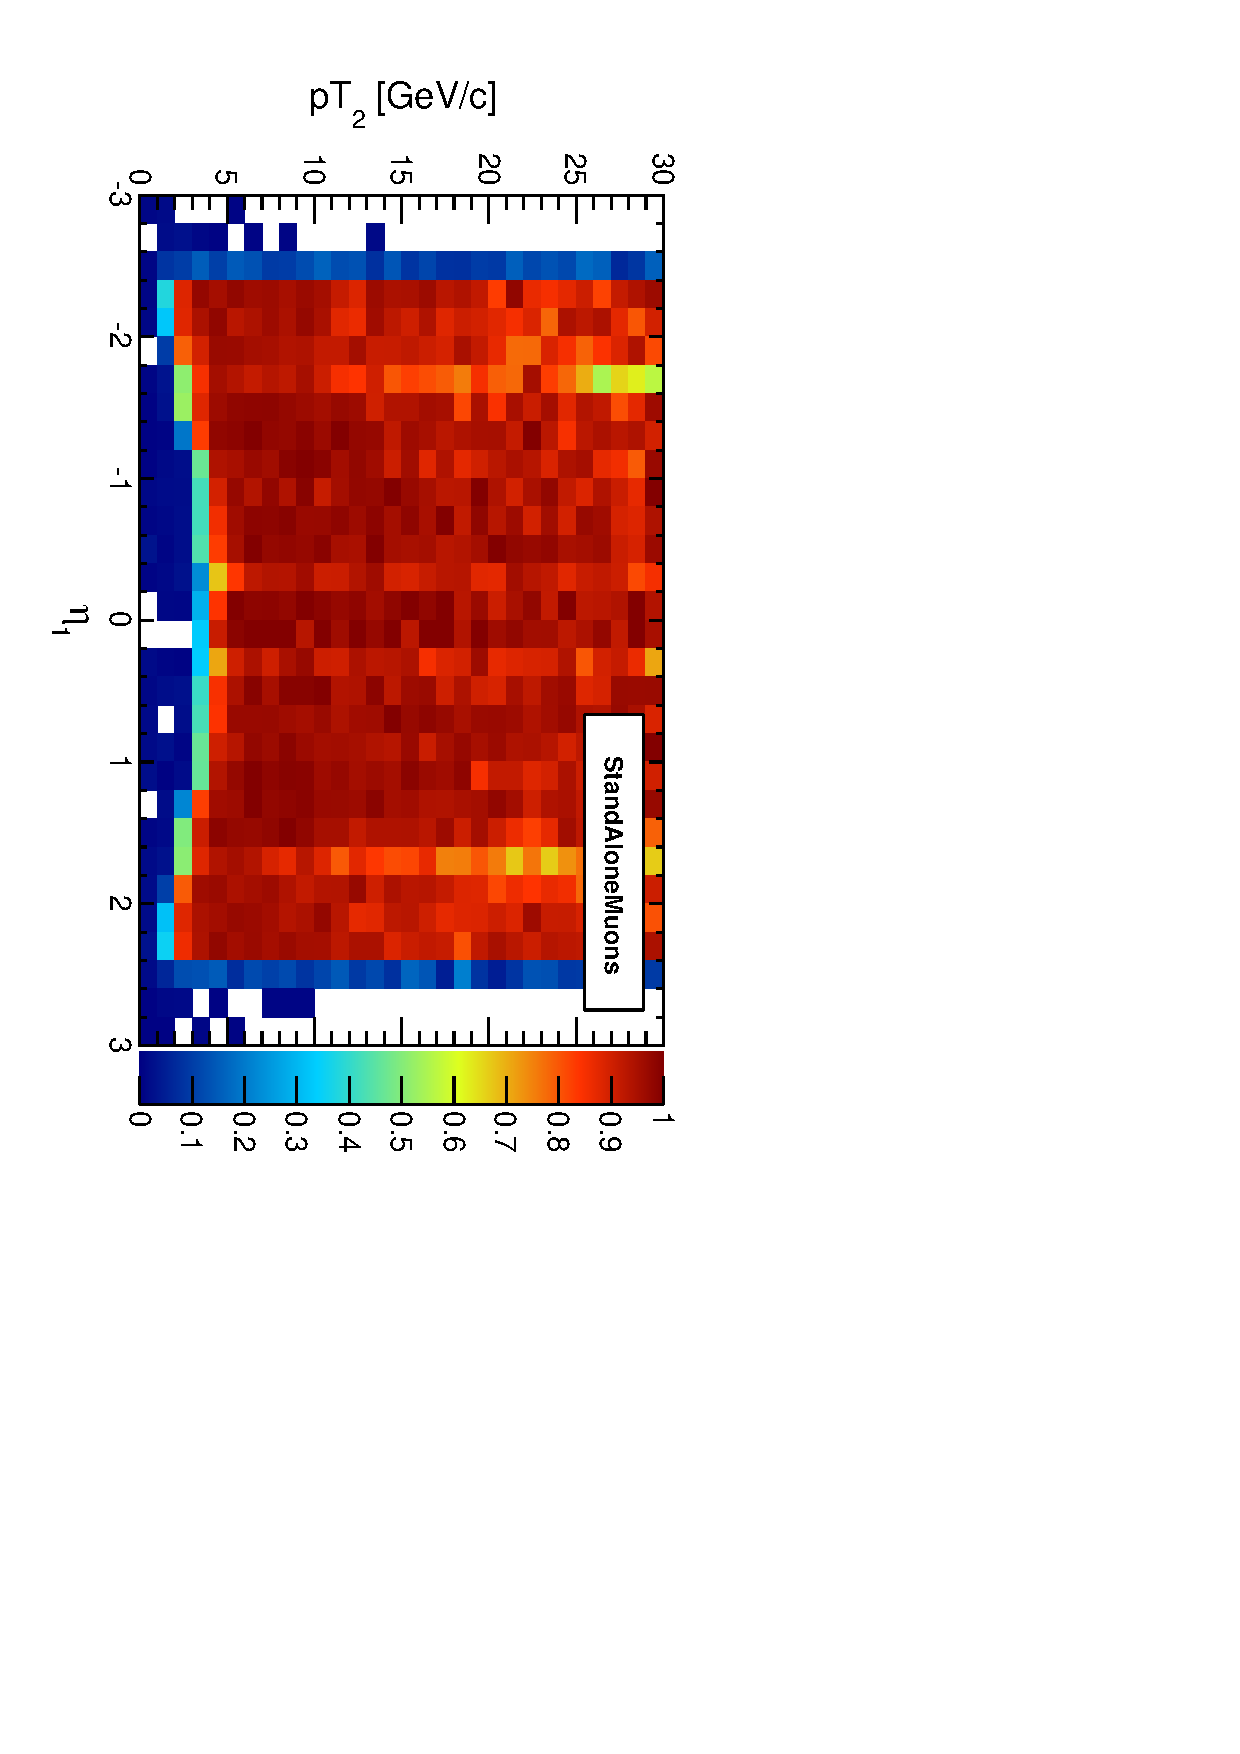
\includegraphics[height=0.45\linewidth, angle=90]{pt2vseta1_StandAloneUpdatedDefault.pdf}

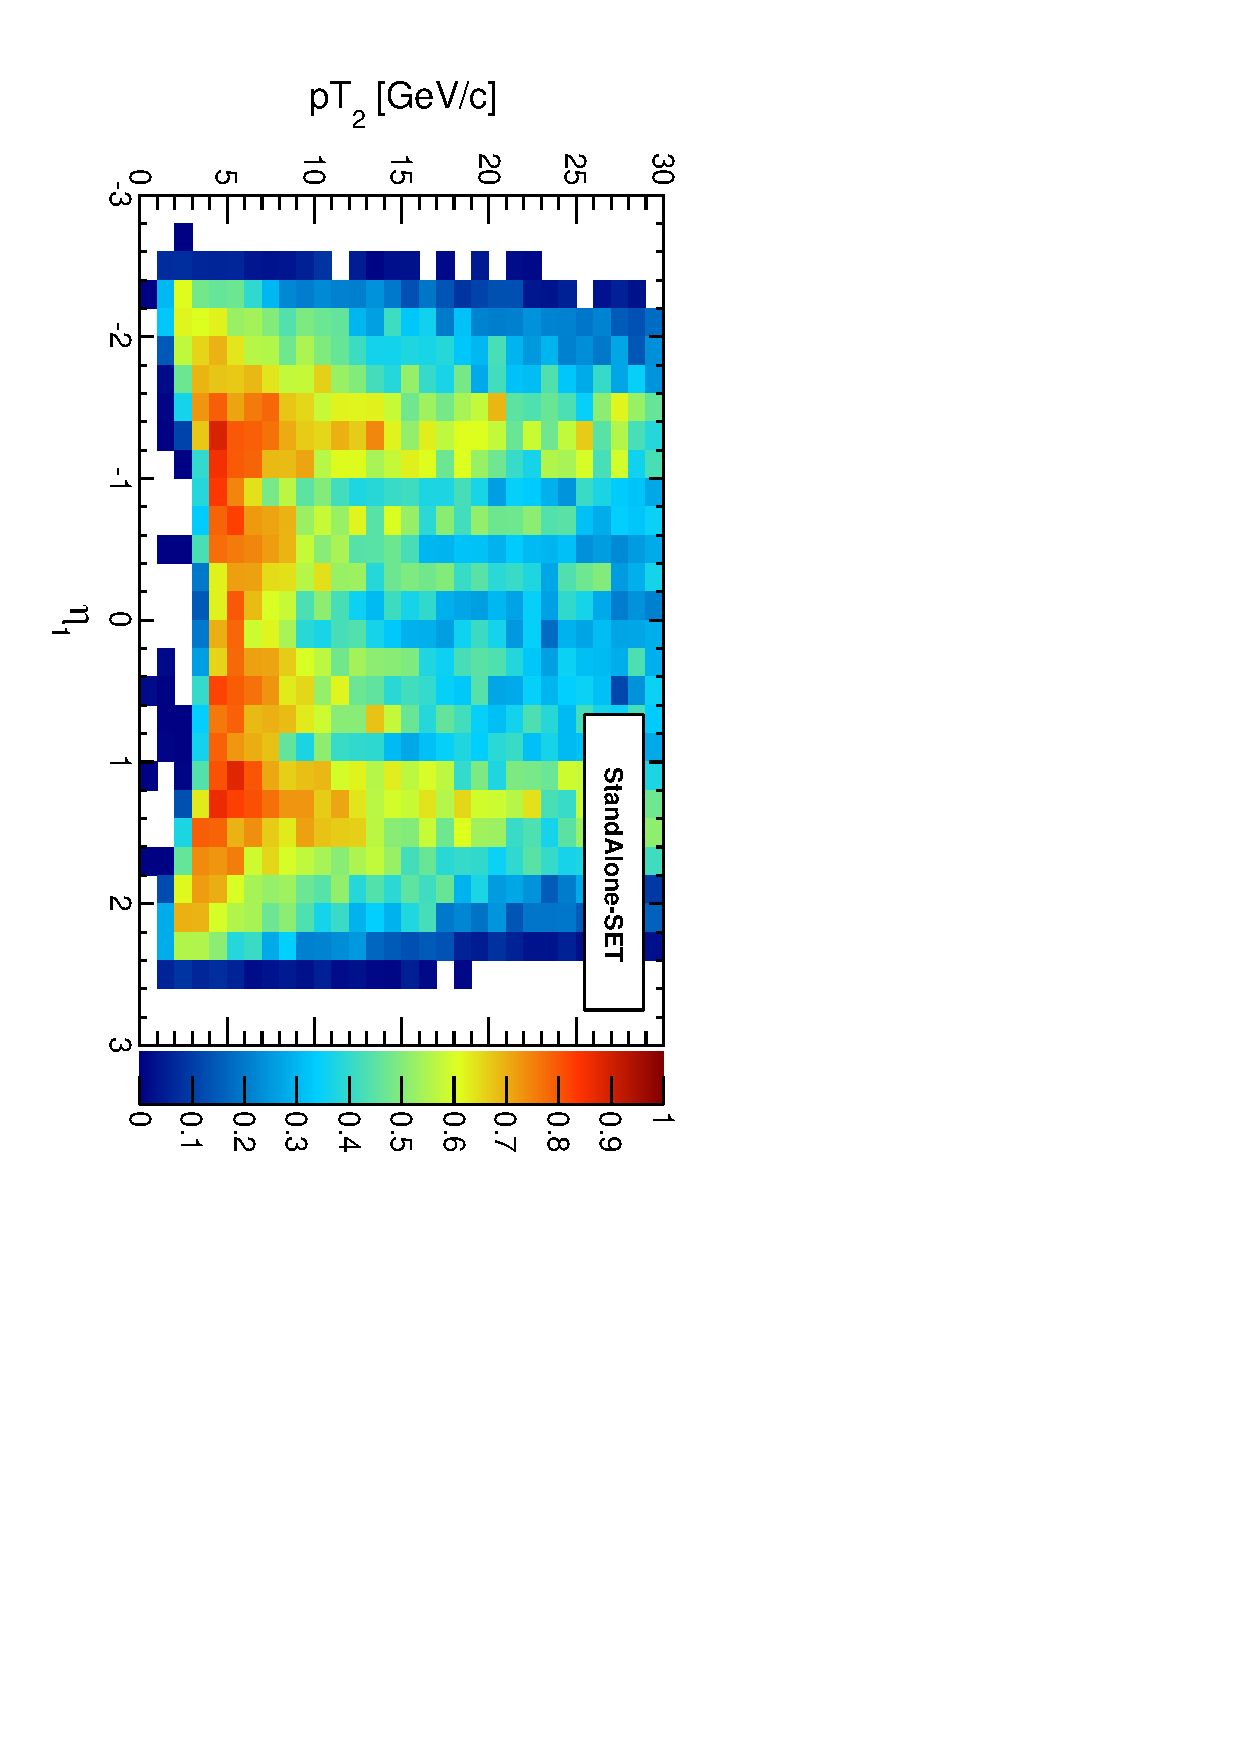
\includegraphics[height=0.45\linewidth, angle=90]{pt2vseta1_StandAloneUpdatedSET.pdf}
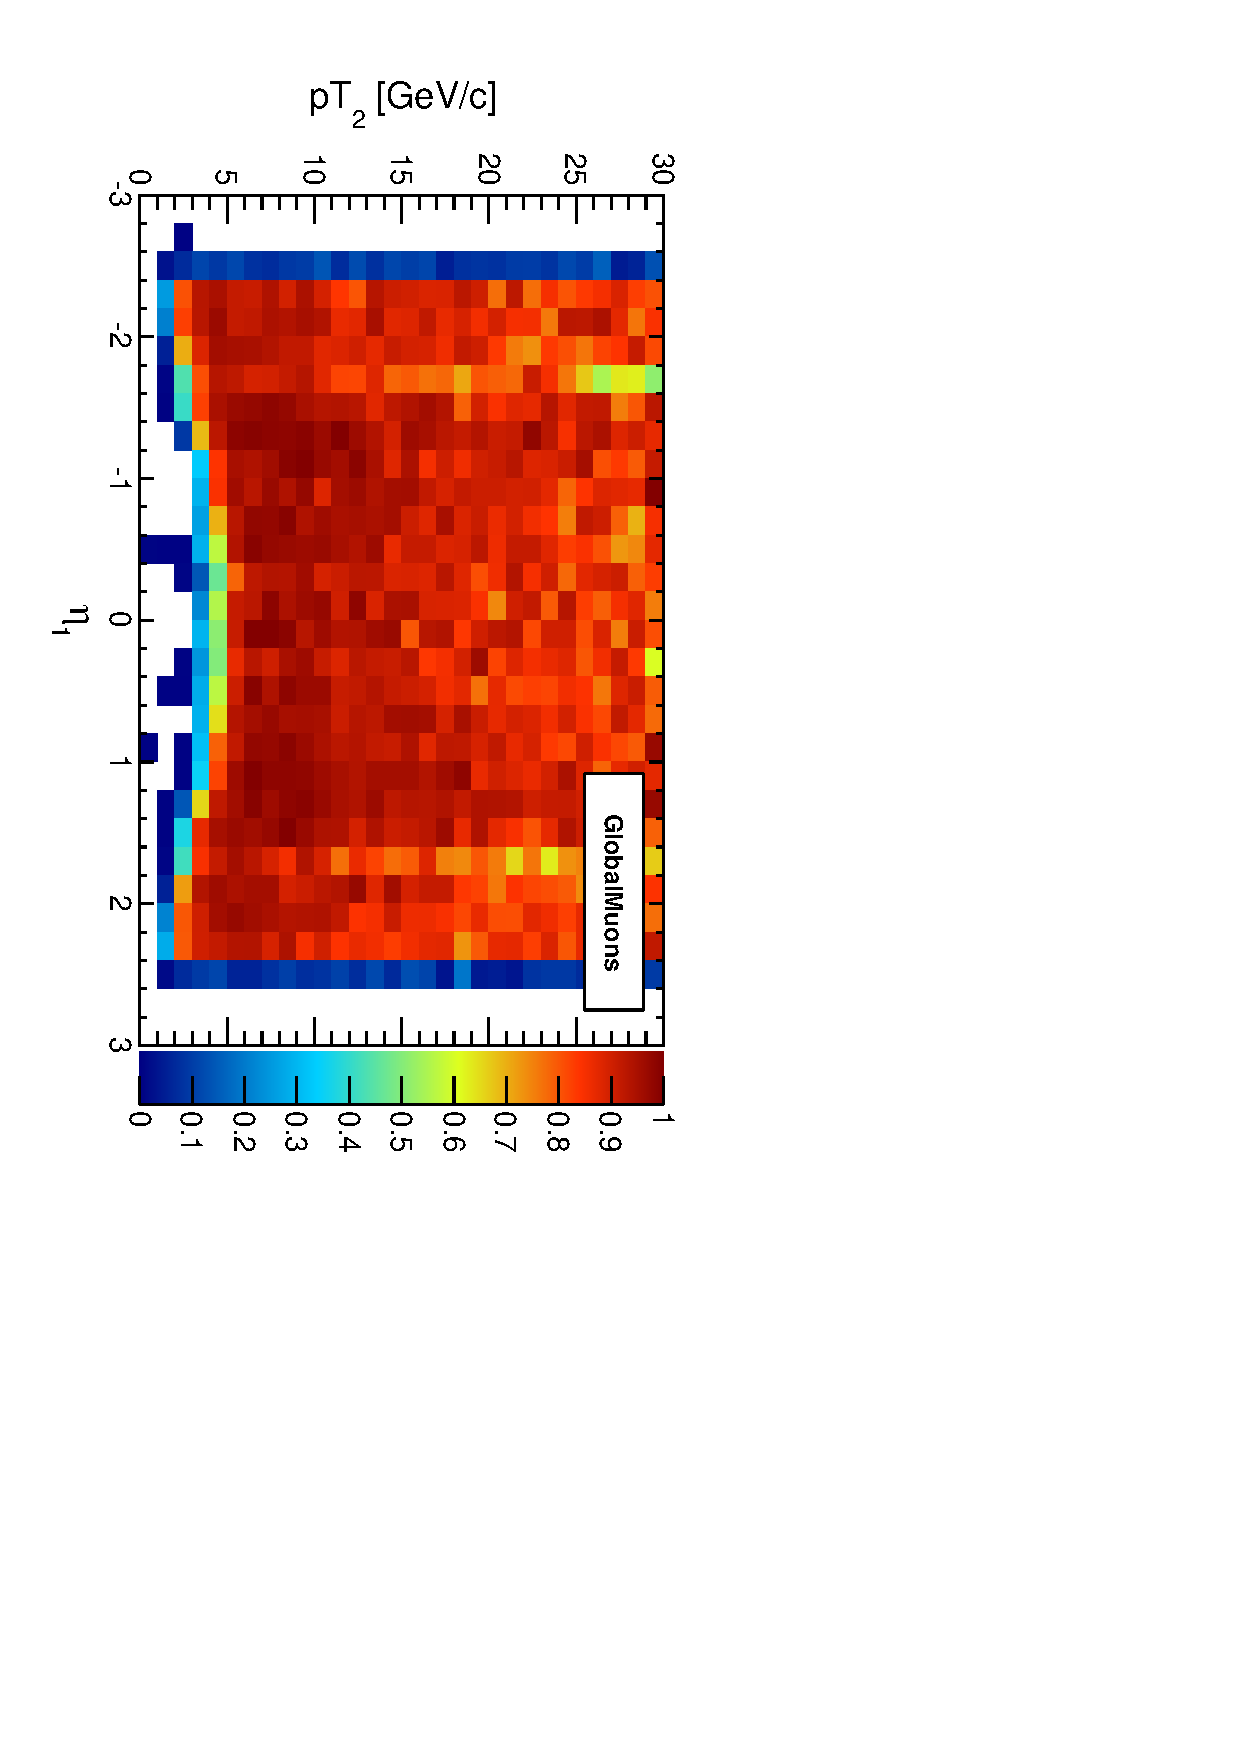
\includegraphics[height=0.45\linewidth, angle=90]{pt2vseta1_GlobalMuons.pdf}
\end{center}
\end{frame}

\begin{frame}
\frametitle{TrackerMuons vs.\ GlobalMuons}
\begin{itemize}\setlength{\itemsep}{0.25 cm}
\item TrackerMuons have high efficiency everywhere, but they also have (curably) high backgrounds
\item StandAloneMuon efficiency depends on how close the muons approach each other in the muon system (next slide)
\item GlobalMuon efficiency $\le$ StandAloneMuon efficiency
\begin{itemize}
\item probability of crossing in the muon system depends on kinematics of the decay
\item this would make it more complicated to quote limits on Lepton Jets derived from GlobalMuons
\end{itemize}
\item I tried StandAlone-SET because I knew that it is an alternative to the standard StandAloneMuons
\begin{itemize}
\item it wasn't designed for nearby-muon efficiency
\item we won't be using it
\end{itemize}
\end{itemize}
\end{frame}

\begin{frame}
\frametitle{Efficiency vs.\ crossing}
\begin{itemize}
\item StandAloneMuon inefficiencies are driven by reconstruction
  issues for muons that overlap in the muon system
\item Test: propagate generator-level muons to planes of constant-$z$
  in the endcap and cylinders around the beamline in the barrel
\item Plot efficiency as a function of trajectory intersections:
  $\Delta \phi_\s{ME2}$ is $\phi_{\mu^+} - \phi_{\mu^-}$ at $z =
  828.561$~cm, $\Delta R\s{ME2}$ is radial difference
\end{itemize}
\begin{center}
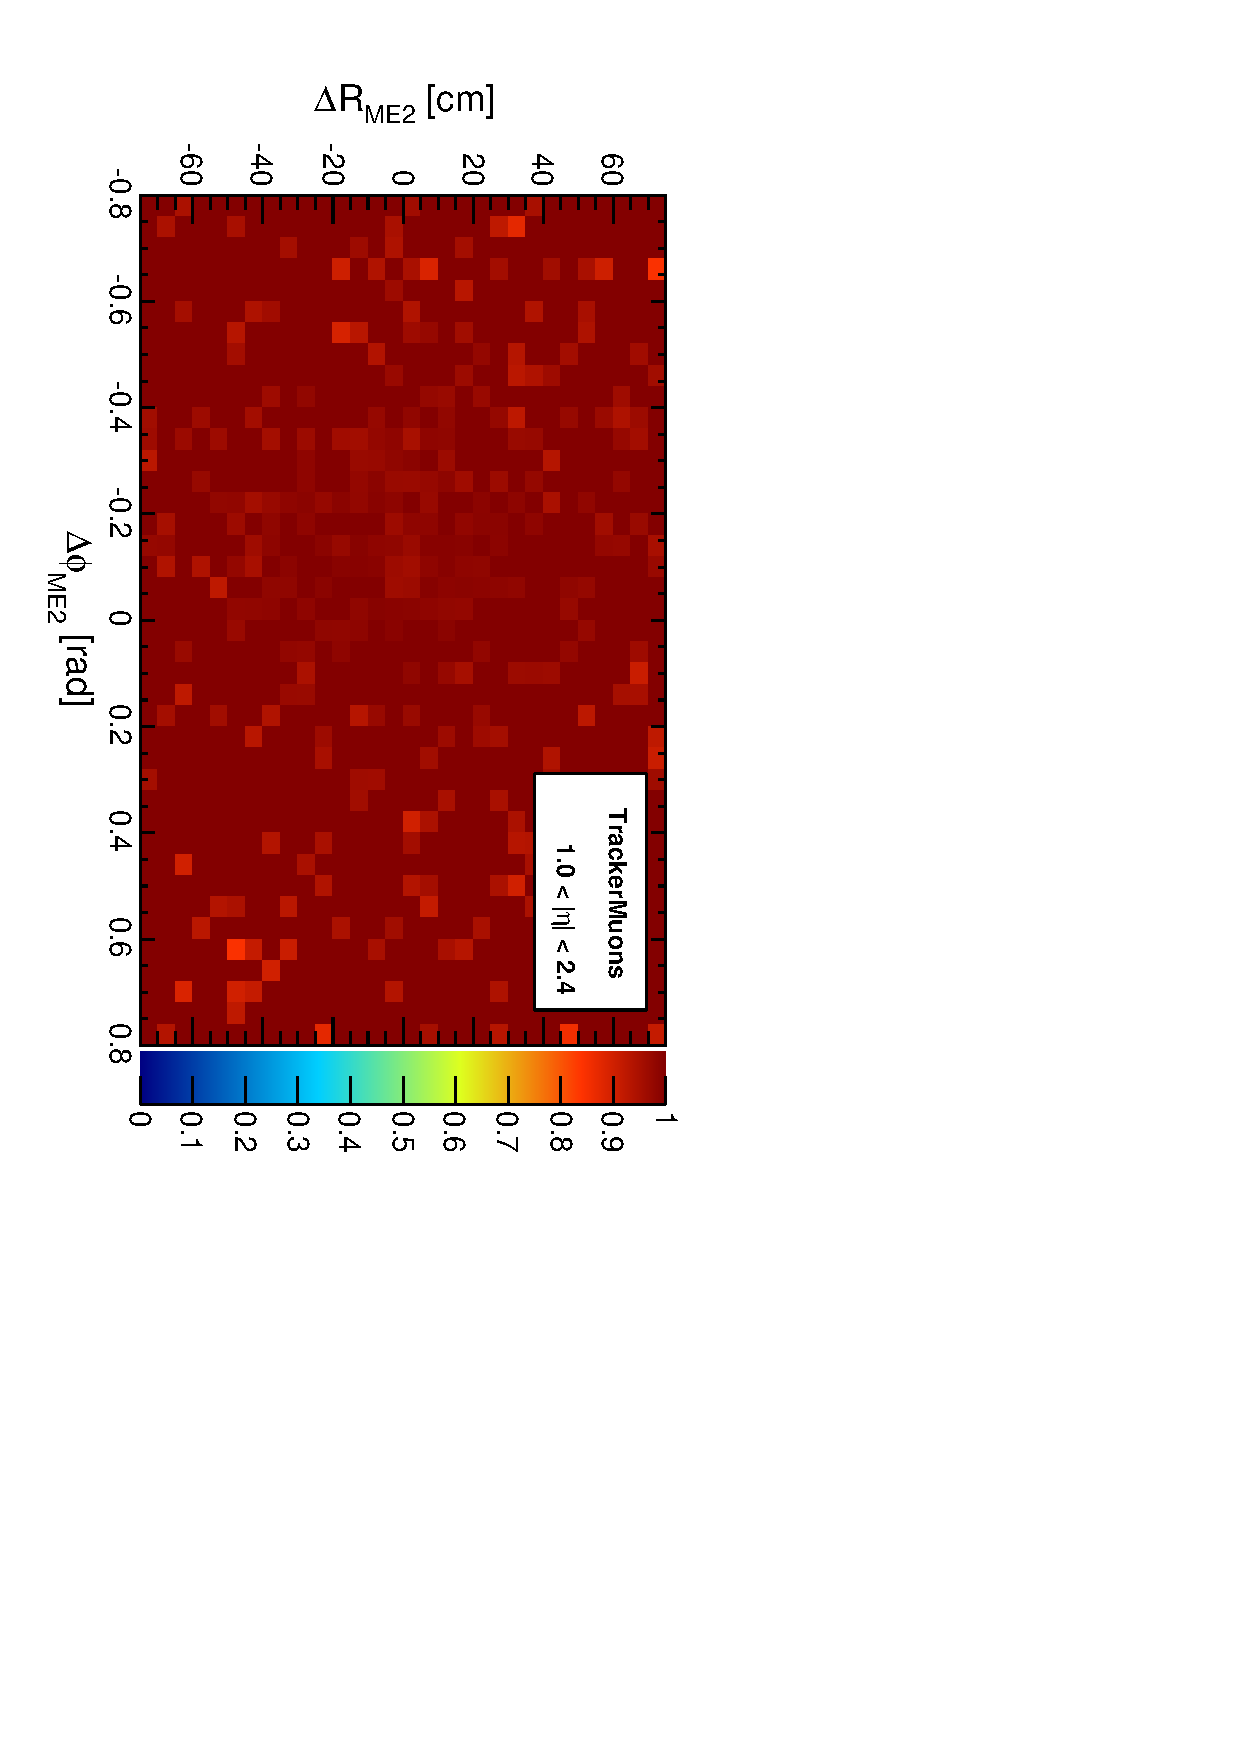
\includegraphics[height=0.45\linewidth, angle=90]{me2_TrackerMuons.pdf}
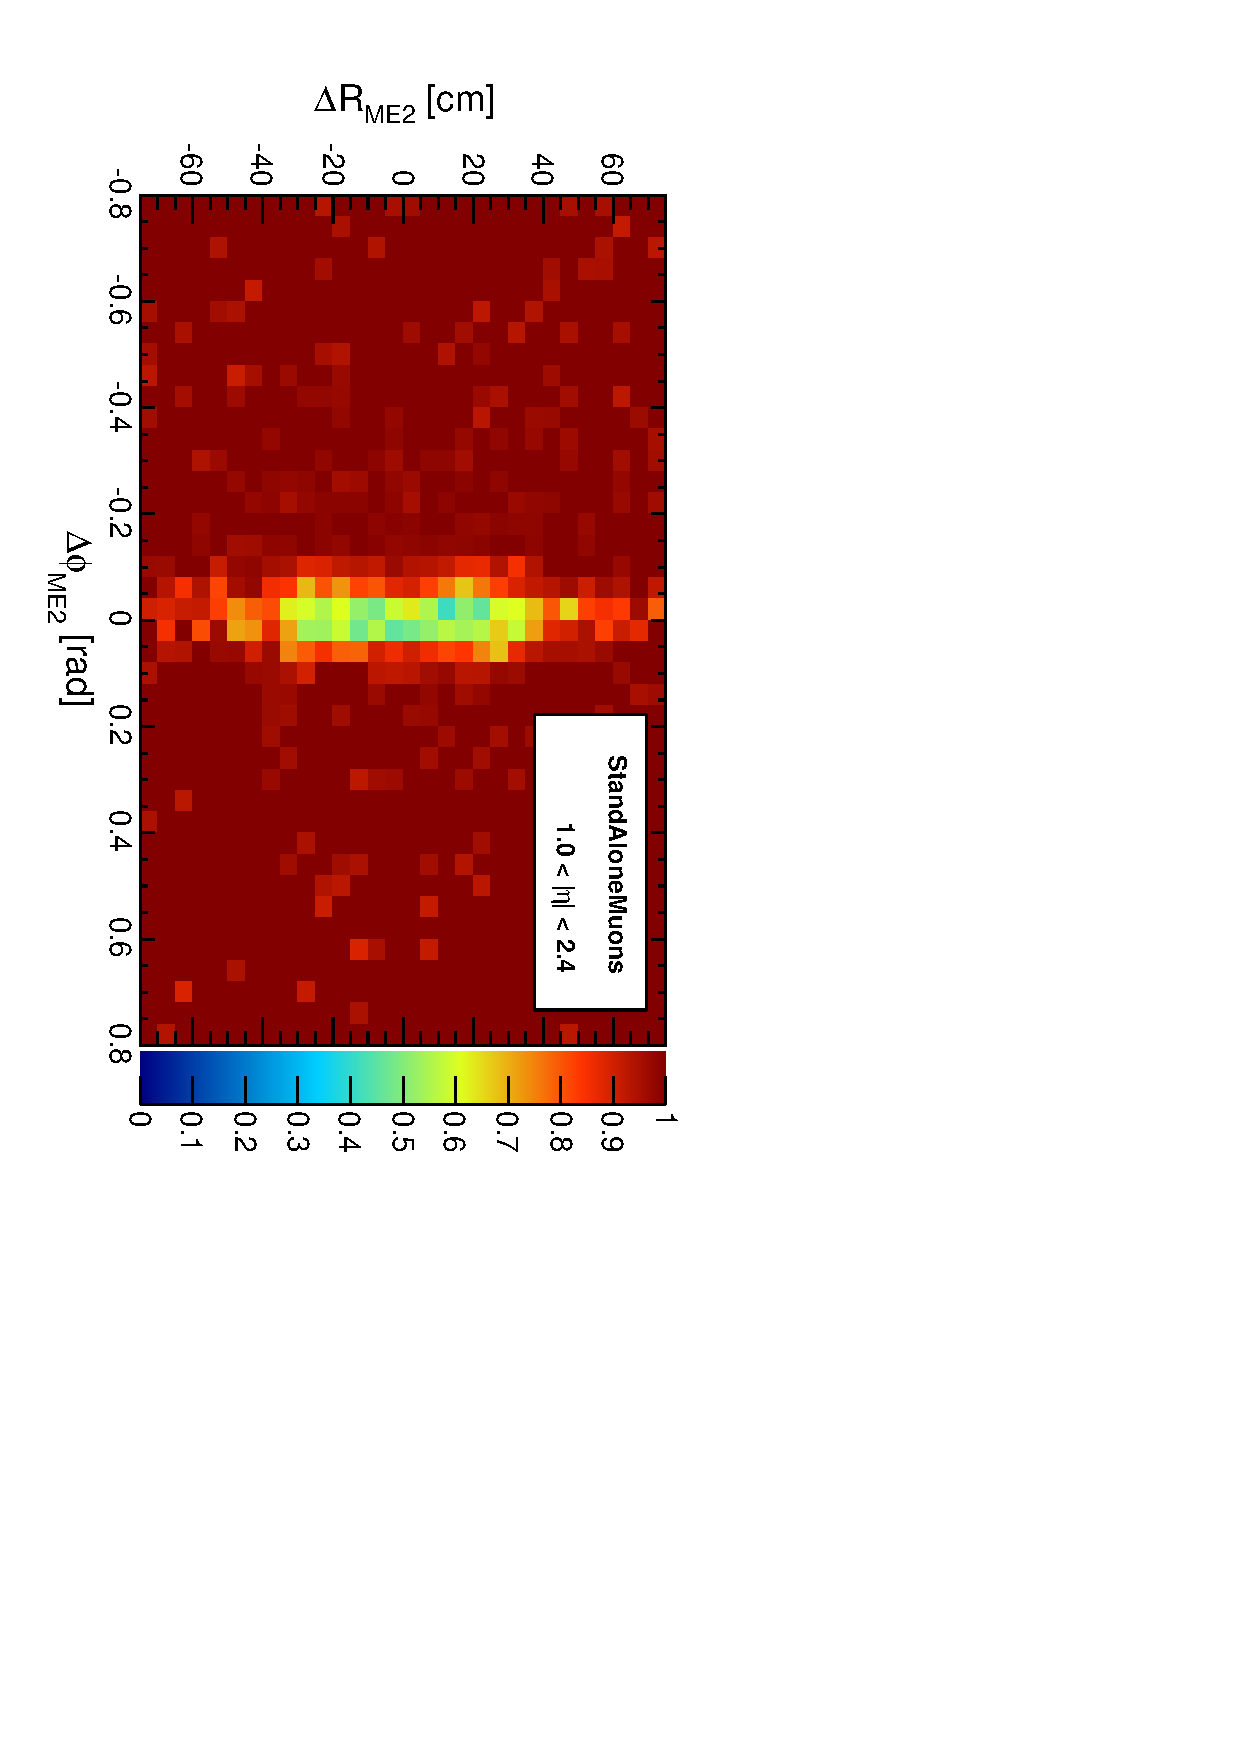
\includegraphics[height=0.45\linewidth, angle=90]{me2_StandAloneUpdatedDefault.pdf}

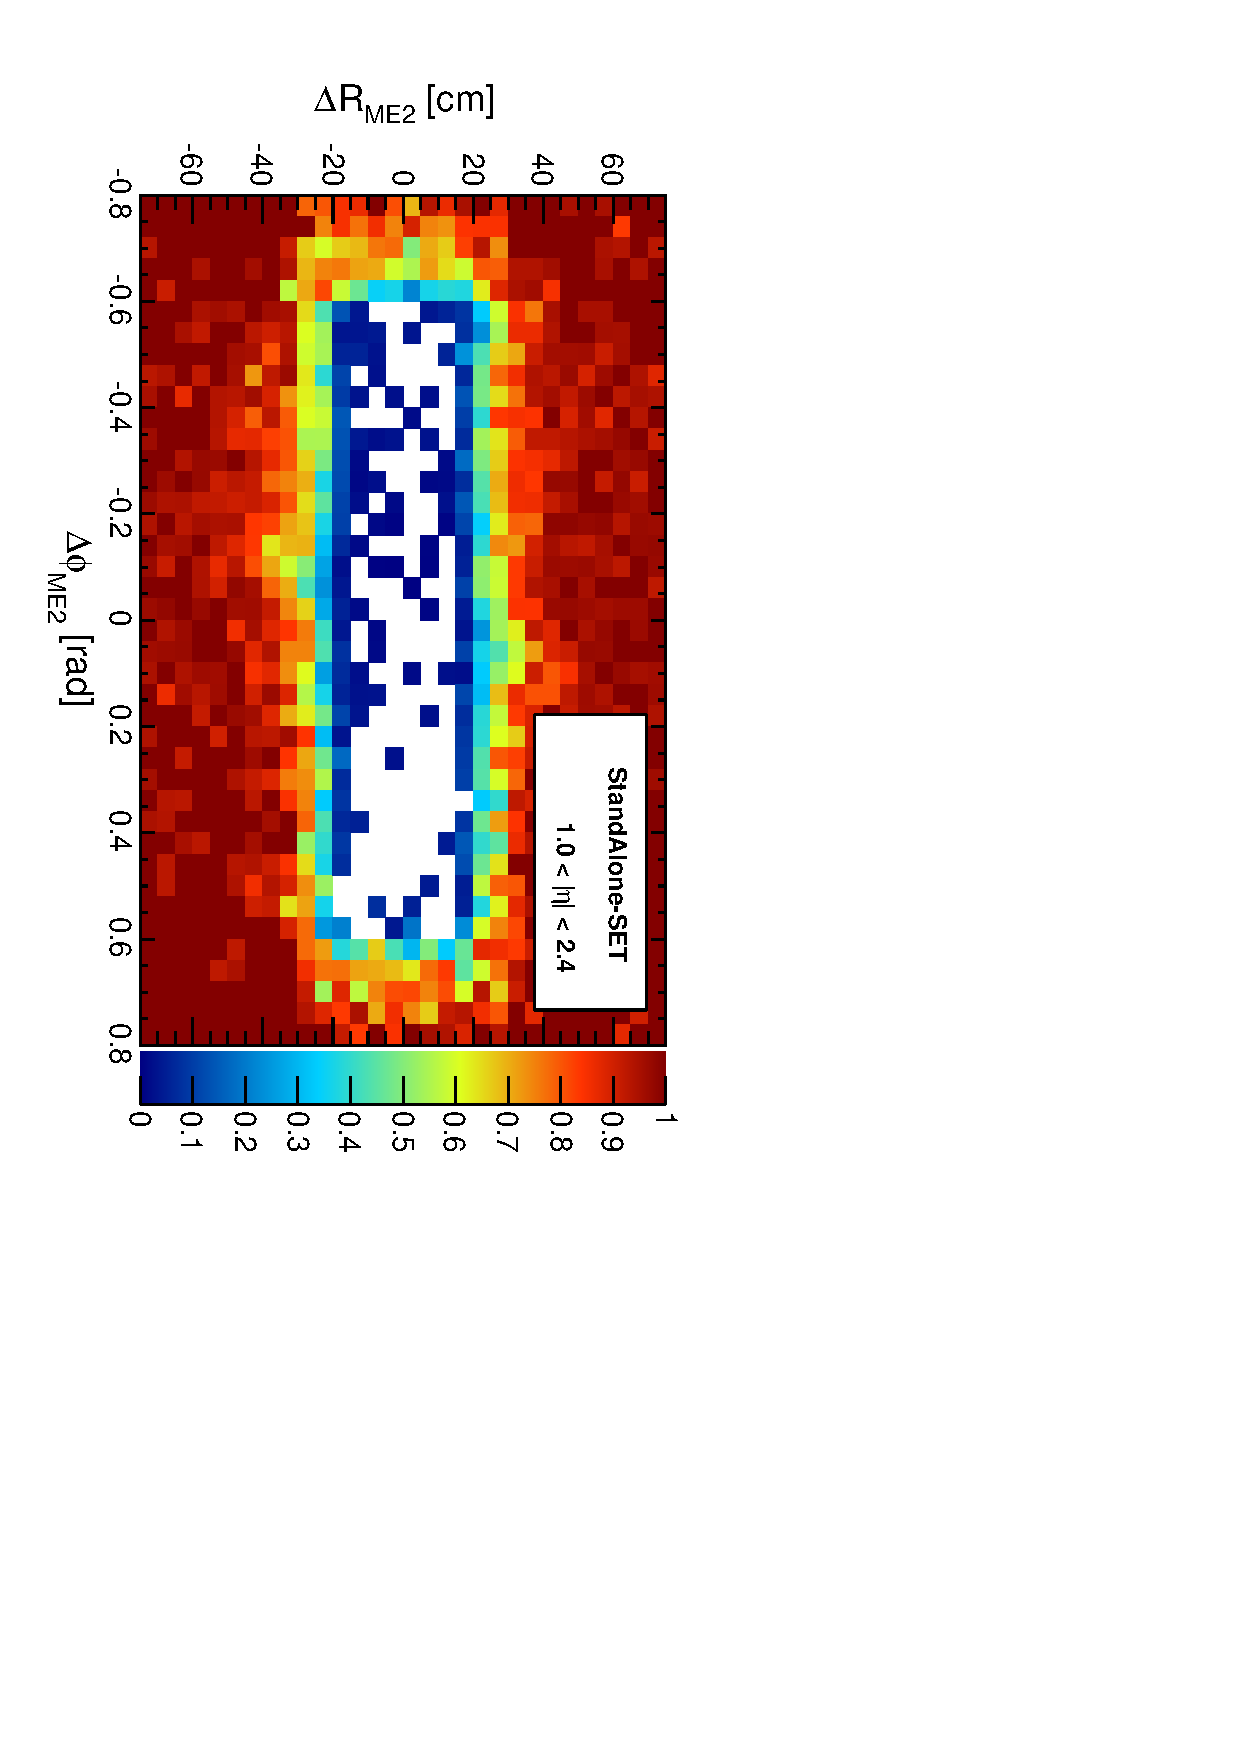
\includegraphics[height=0.45\linewidth, angle=90]{me2_StandAloneUpdatedSET.pdf}
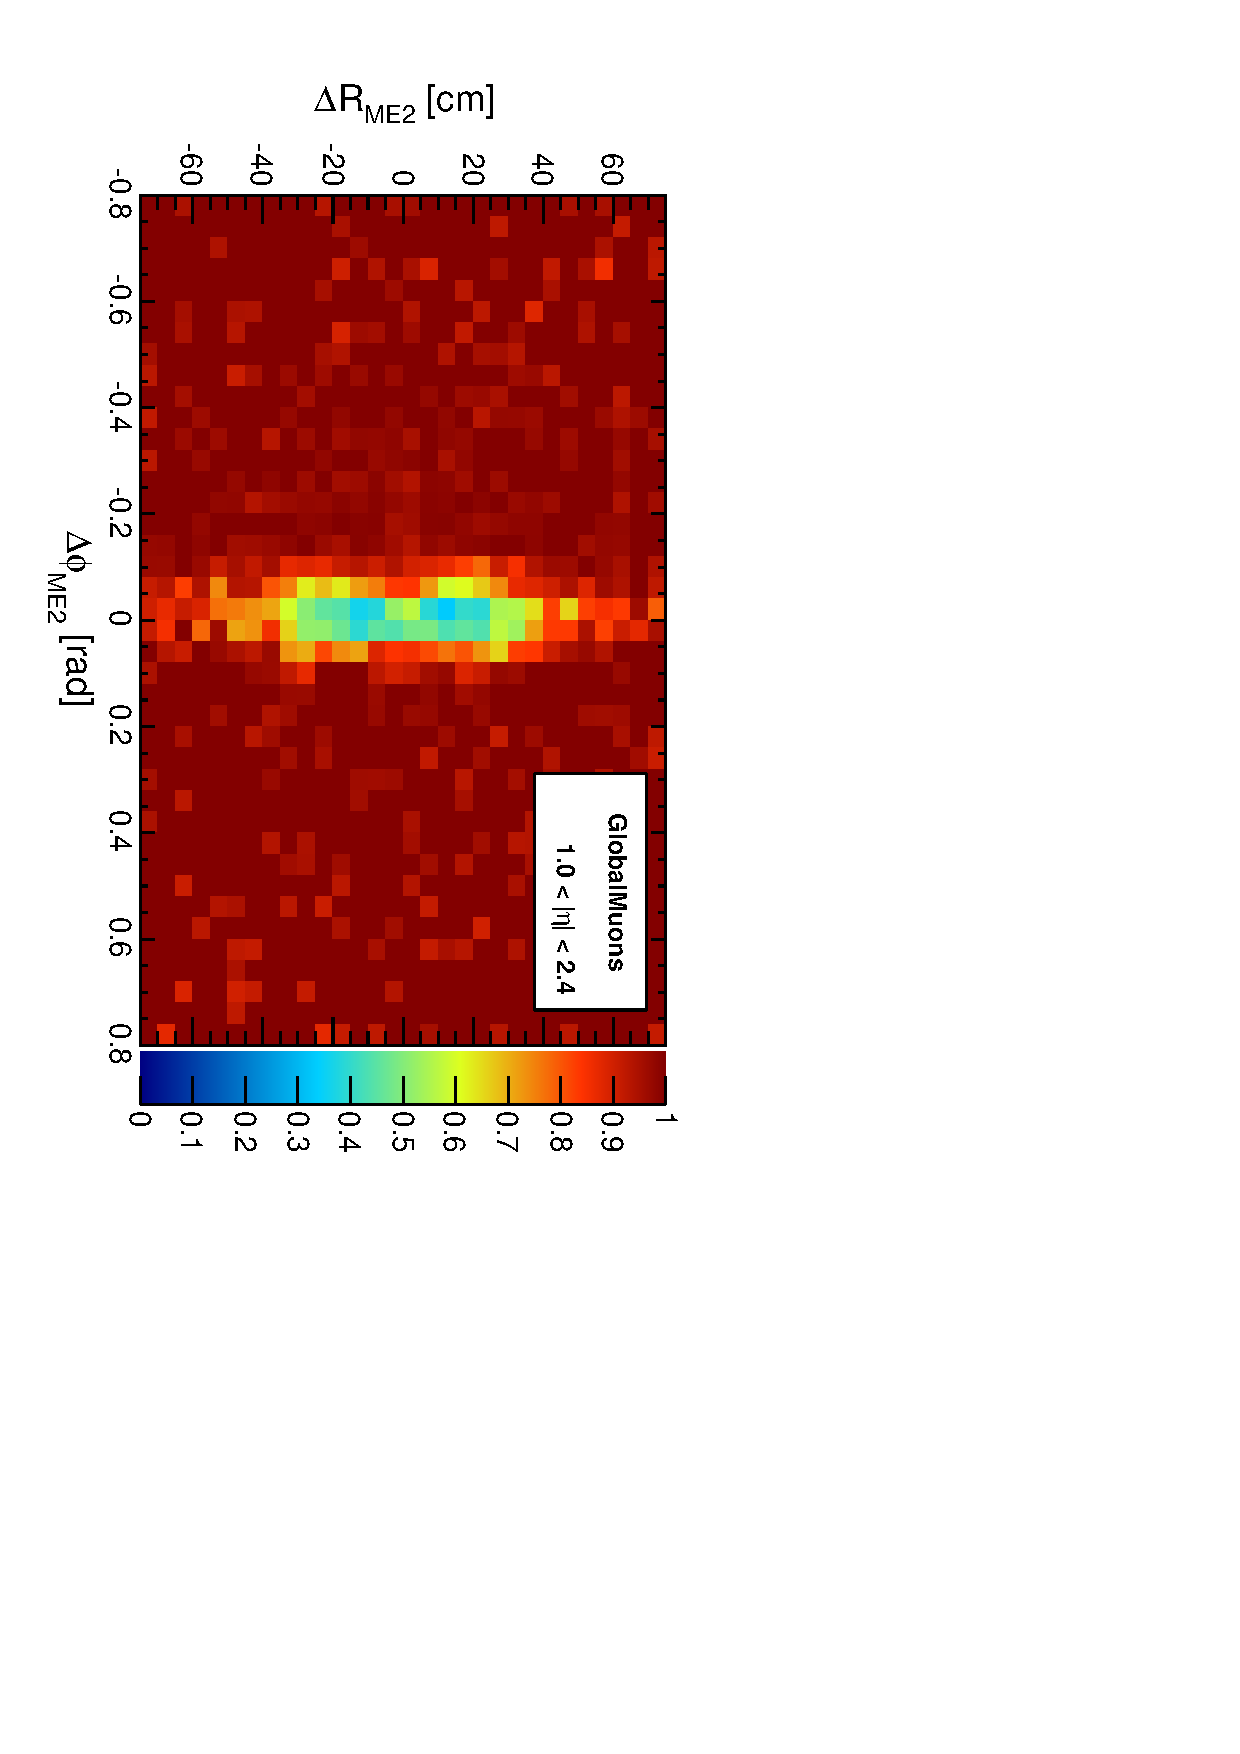
\includegraphics[height=0.45\linewidth, angle=90]{me2_GlobalMuons.pdf}
\end{center}
\end{frame}

\begin{frame}
\frametitle{Efficiency vs.\ crossing}
\begin{itemize}
\item Same thing in the barrel: $\Delta \phi_{MB3}$ and $\Delta
  Z_{MB3}$ on a cylinder of radius 618.269~cm
\item Not completely understood: inefficiencies are off-centered from
  zero
\item Suggests that this plot is ``out of focus''--- the intersection
  that drives inefficiency is perhaps at smaller radius than barrel?
\end{itemize}

\begin{center}
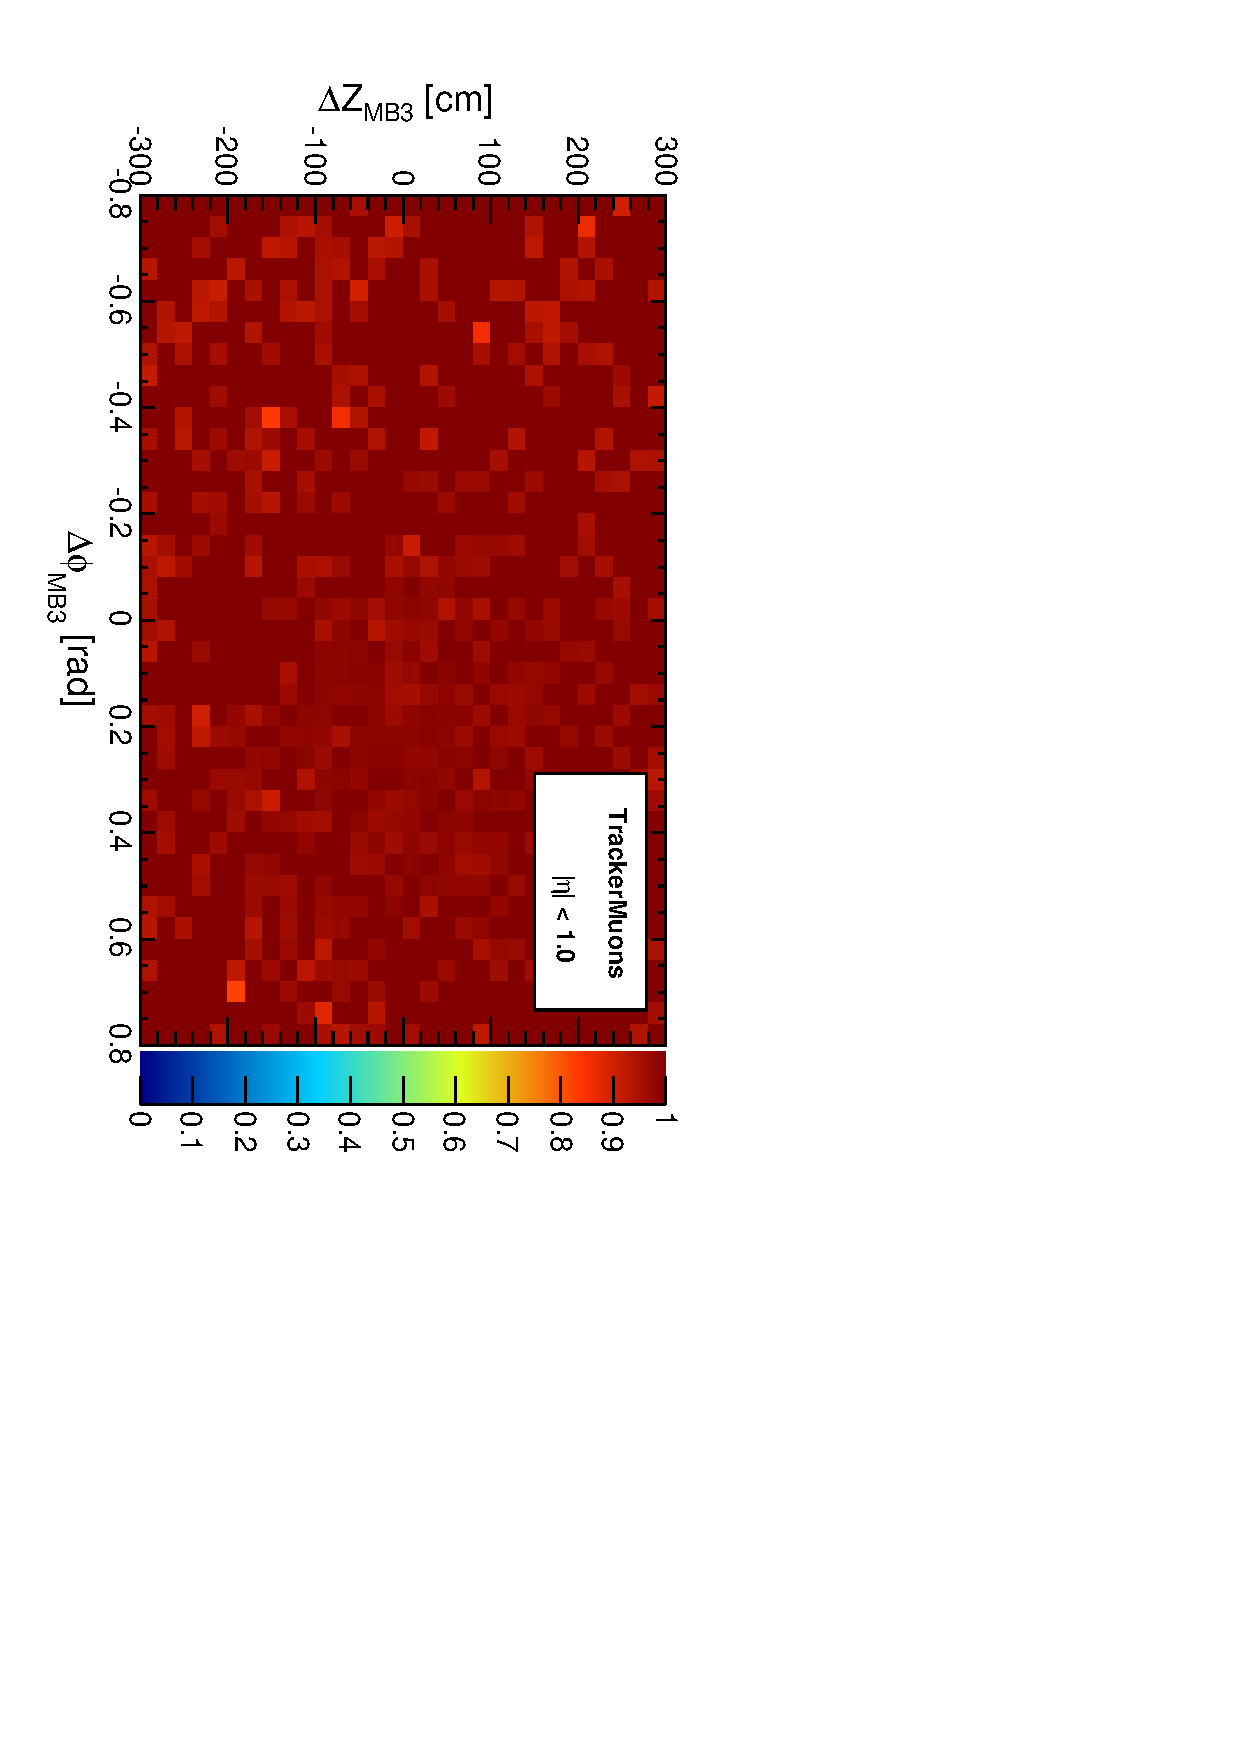
\includegraphics[height=0.45\linewidth, angle=90]{mb3_TrackerMuons.pdf}
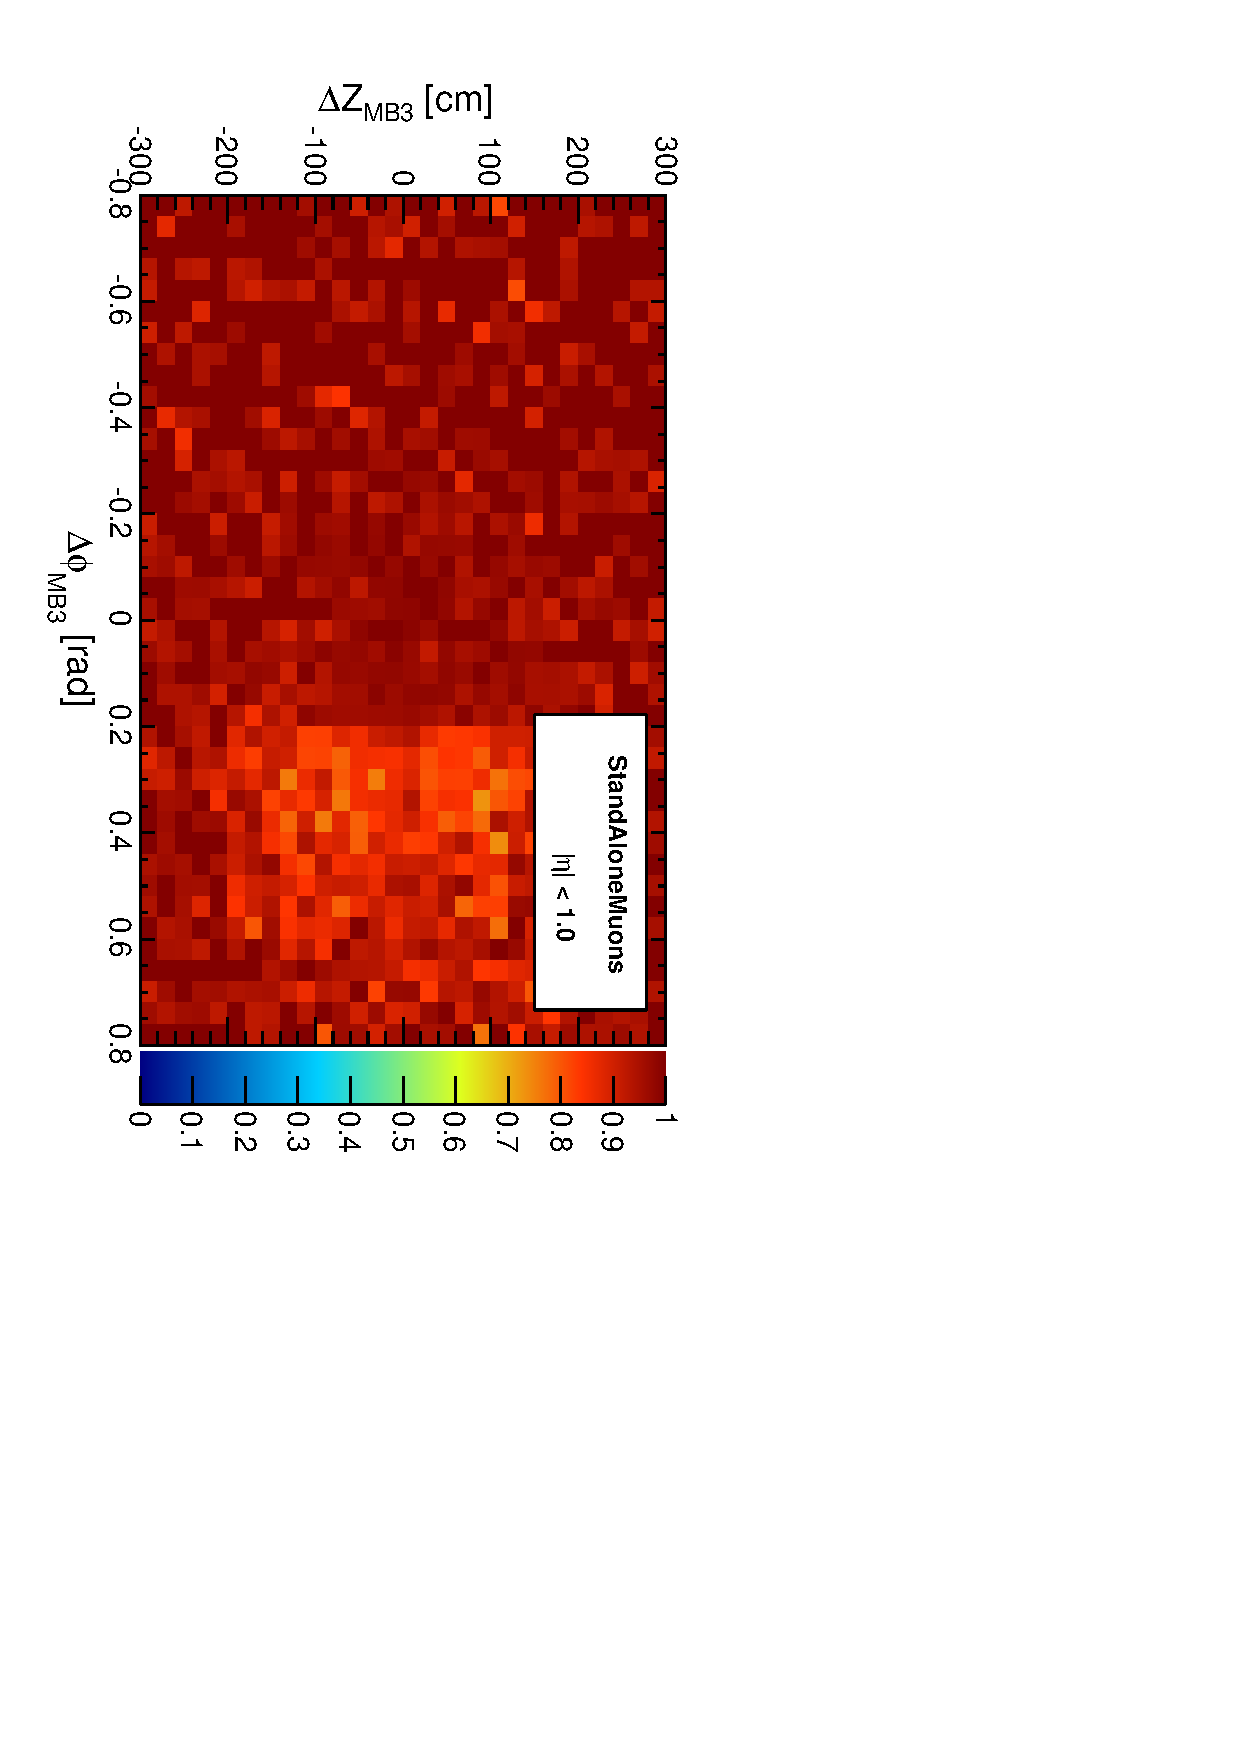
\includegraphics[height=0.45\linewidth, angle=90]{mb3_StandAloneUpdatedDefault.pdf}

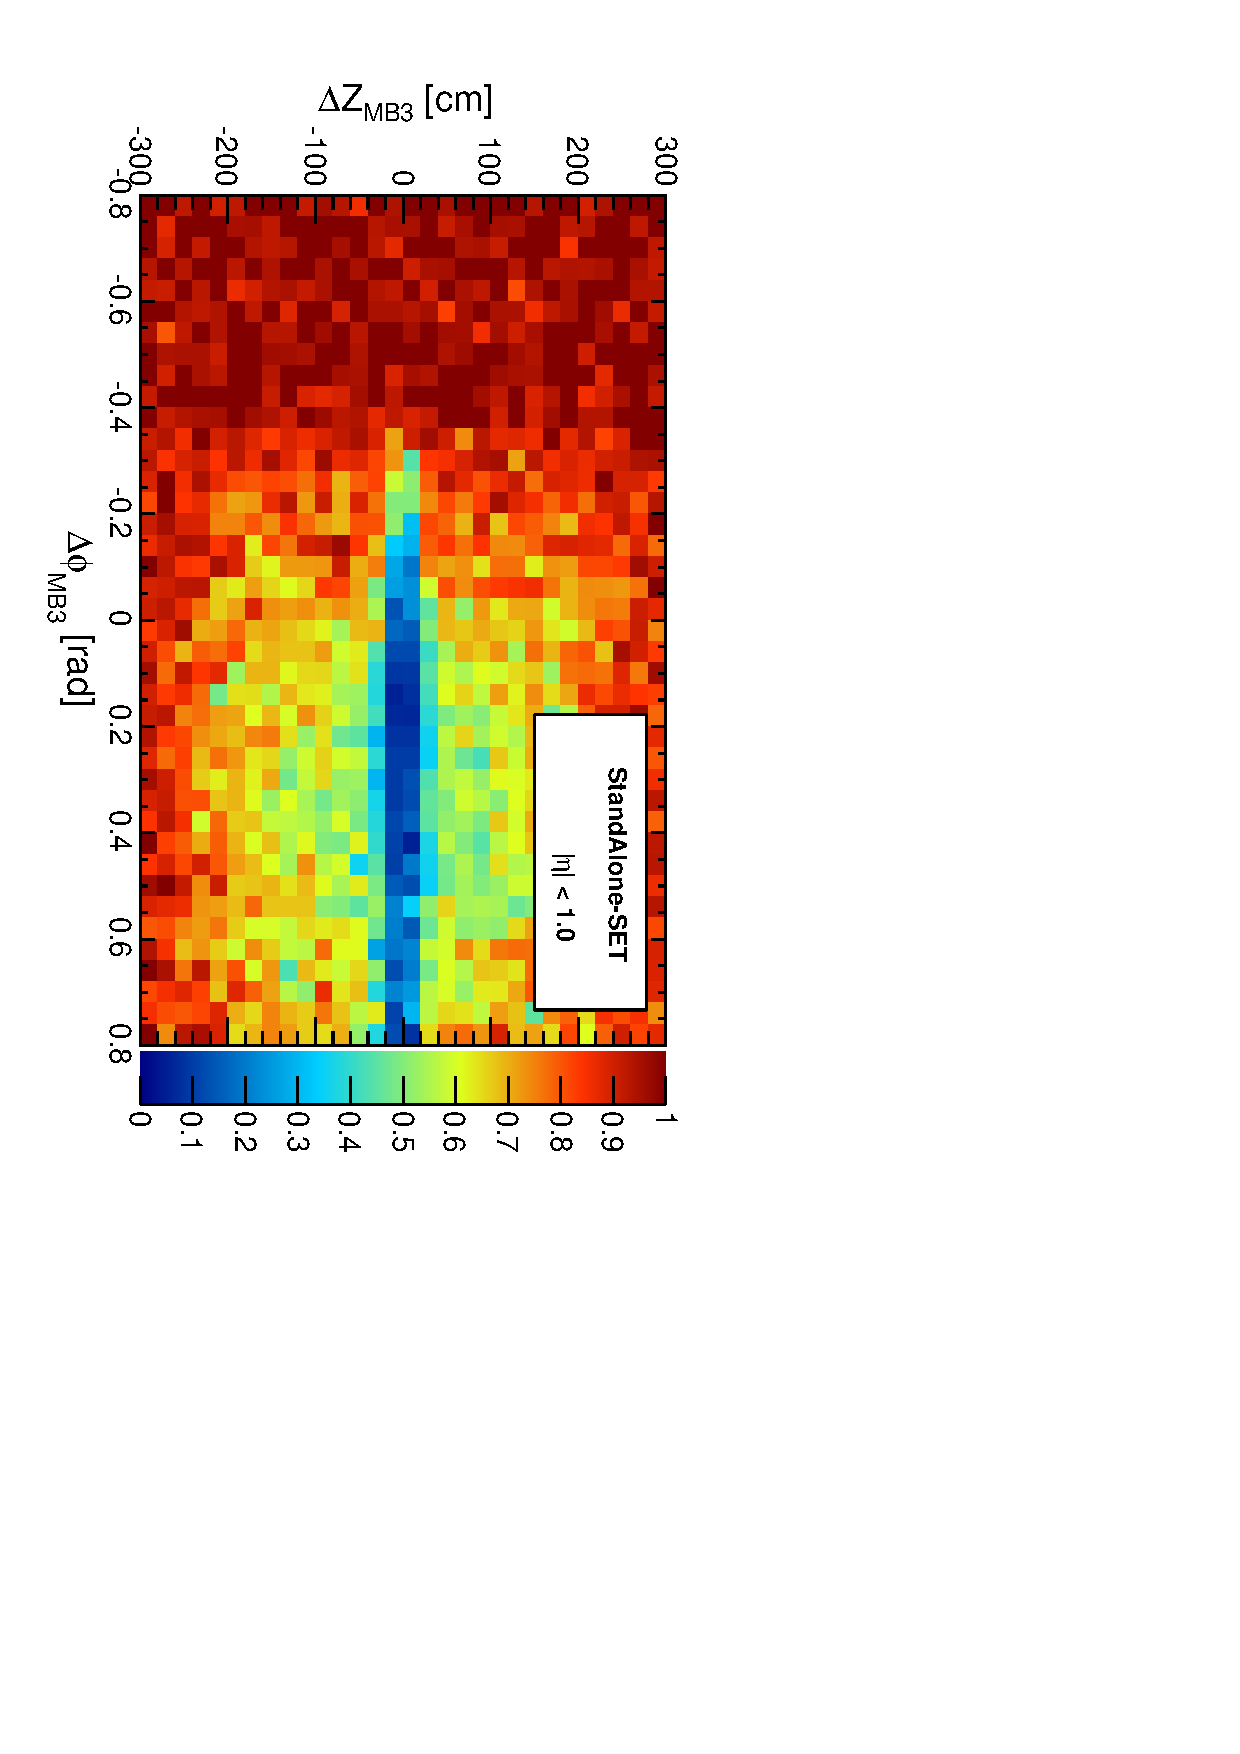
\includegraphics[height=0.45\linewidth, angle=90]{mb3_StandAloneUpdatedSET.pdf}
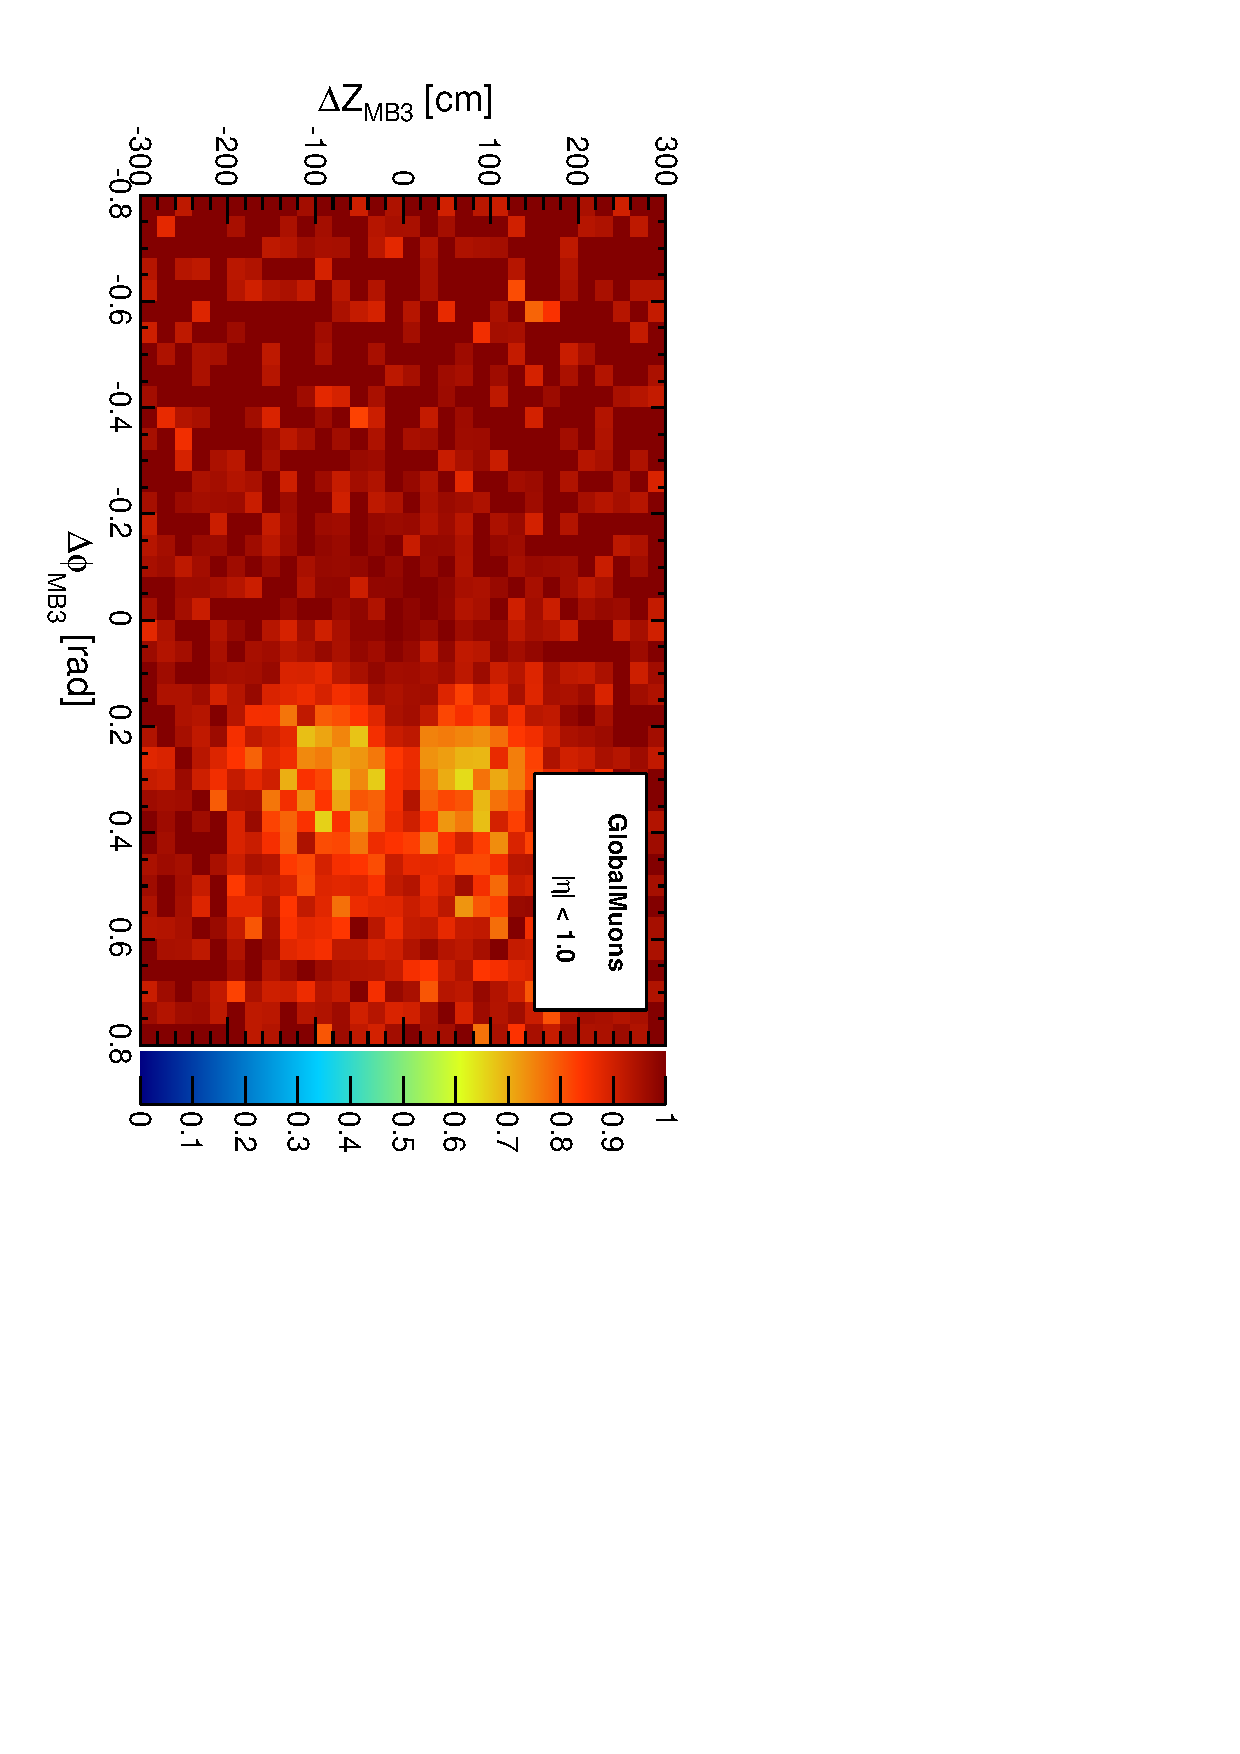
\includegraphics[height=0.45\linewidth, angle=90]{mb3_GlobalMuons.pdf}
\end{center}
\end{frame}

\begin{frame}
\frametitle{TrackerMuon Backgrounds}
\begin{itemize}
\item Before moving on, we should address \mbox{backgrounds with TrackerMuons\hspace{-1 cm}}
\item Number of reconstructed muons $N_\s{muons}$ in the InclusiveMu5\_Pt* samples (all QCD backgrounds, including decay-in-flight):

\begin{center}
\begin{columns}
\column{0.75\linewidth}
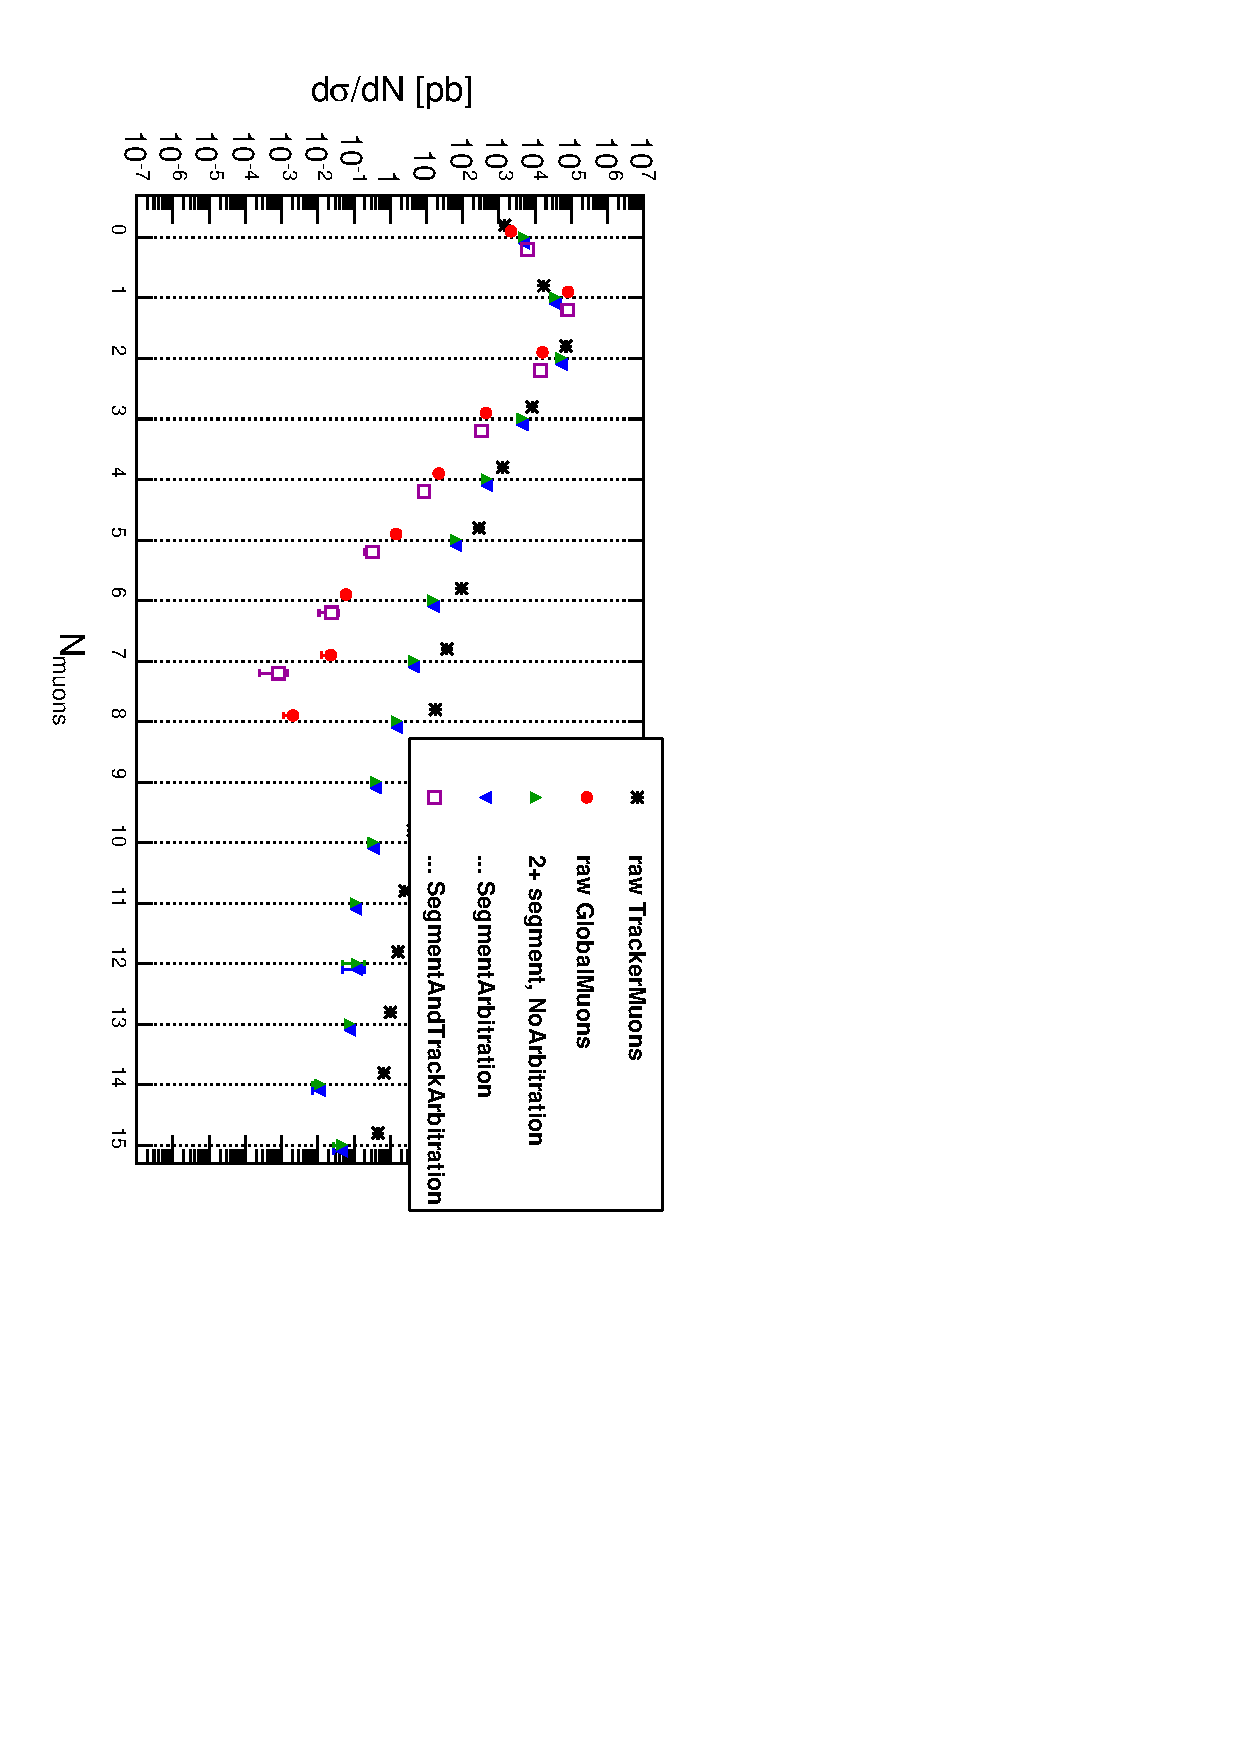
\includegraphics[height=\linewidth, angle=90]{tracks_lastpage_allreal.pdf}

\column{0.25\linewidth}
\scriptsize All sets of track cuts include $p_T > 5$~GeV/$c$

\vspace{0.25 cm} GlobalMuon distributions are nearly independent of sensible cuts
\end{columns}
\end{center}

\item The {\it one cut} that makes TrackerMuons as pure as GlobalMuons
  is $N_\s{segments} \ge 2$ for segment-and-track arbitrated segments
\end{itemize}
\end{frame}

\begin{frame}
\frametitle{TrackerMuon Backgrounds}
\begin{itemize}
\item Same plot, split up by the number of real muons in the event
\begin{itemize}
\item defining ``real muons'' by number of {\it unique} GenParticle muons matched to all reconstructed muons
\end{itemize}

\item As you can see, TrackerMuons with $N_\s{segments} \ge 2$ (open
  purple boxes) are narrowly distributed around the true number of
  muons
\end{itemize}

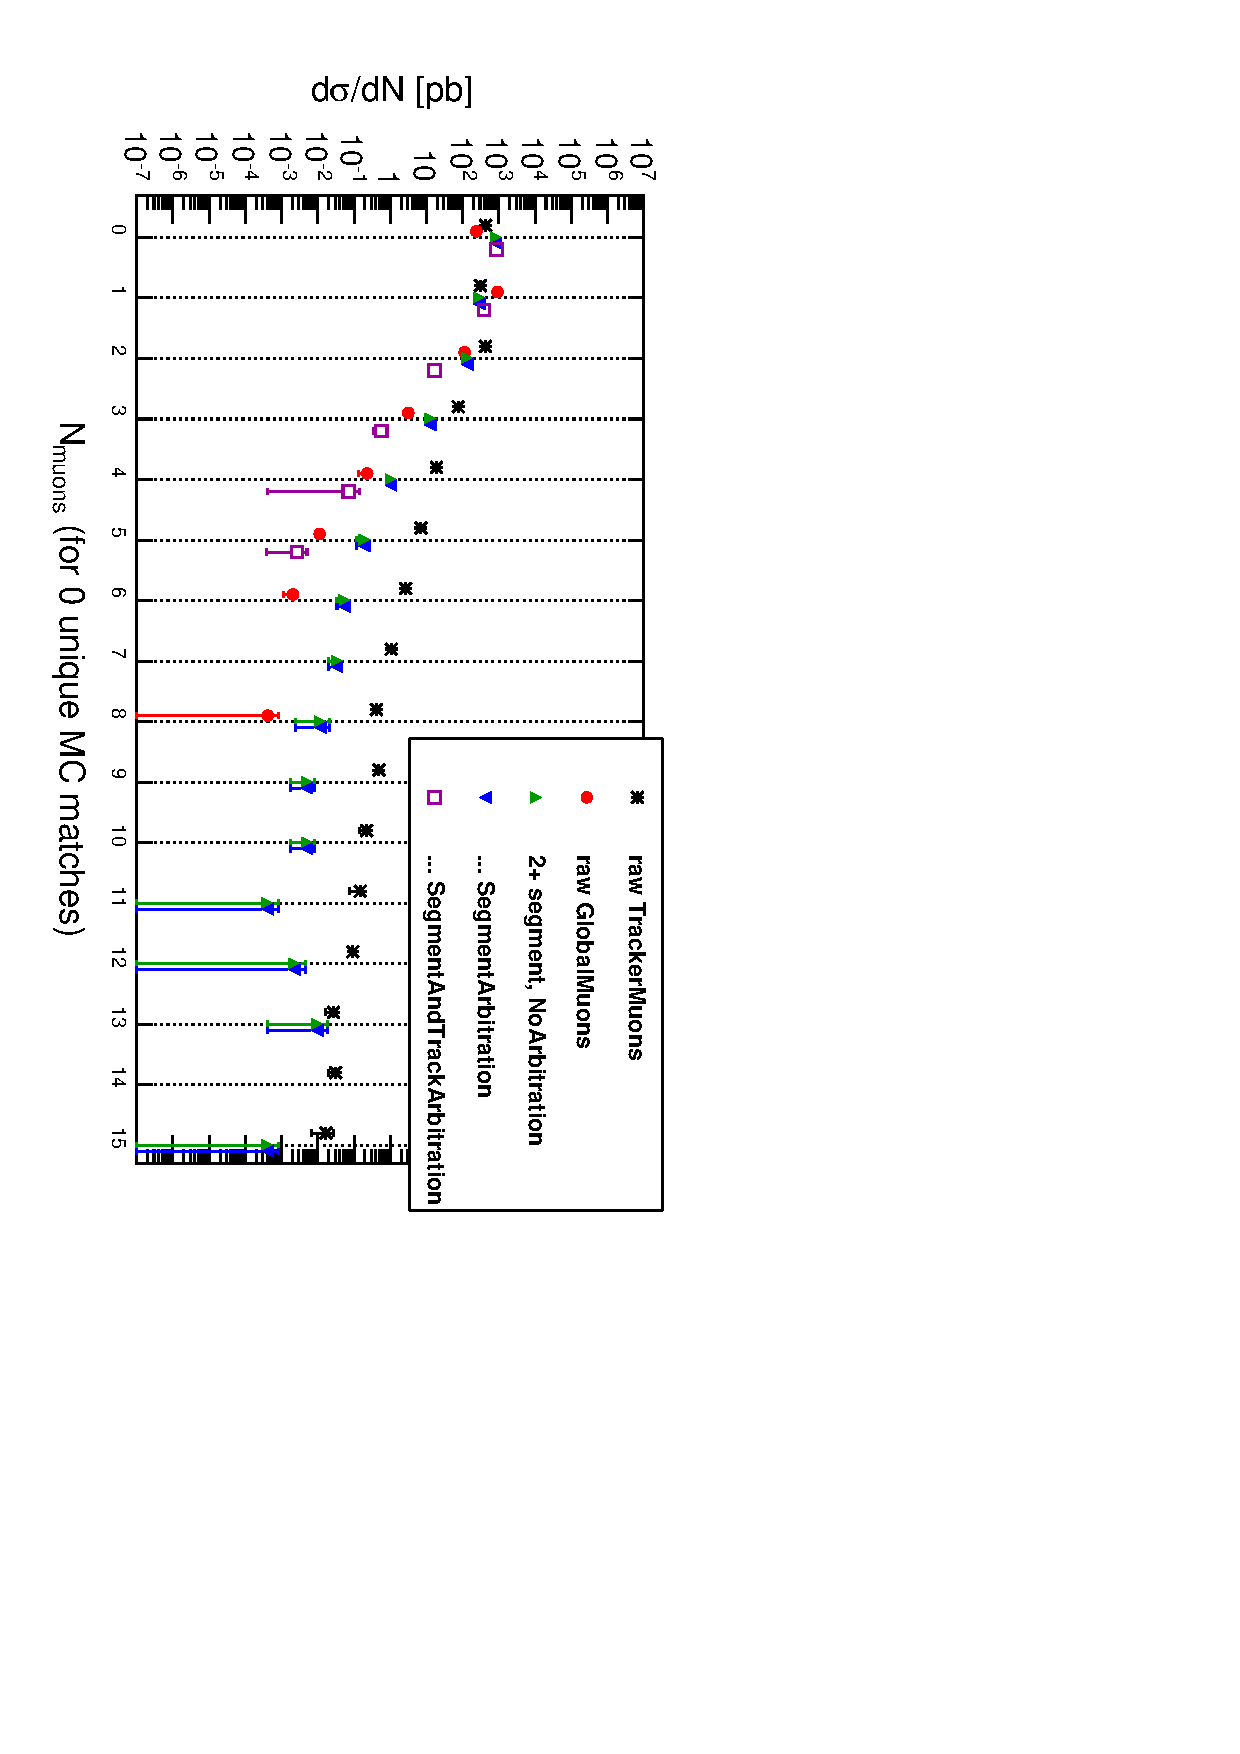
\includegraphics[height=0.5\linewidth, angle=90]{tracks_lastpage_0real.pdf}
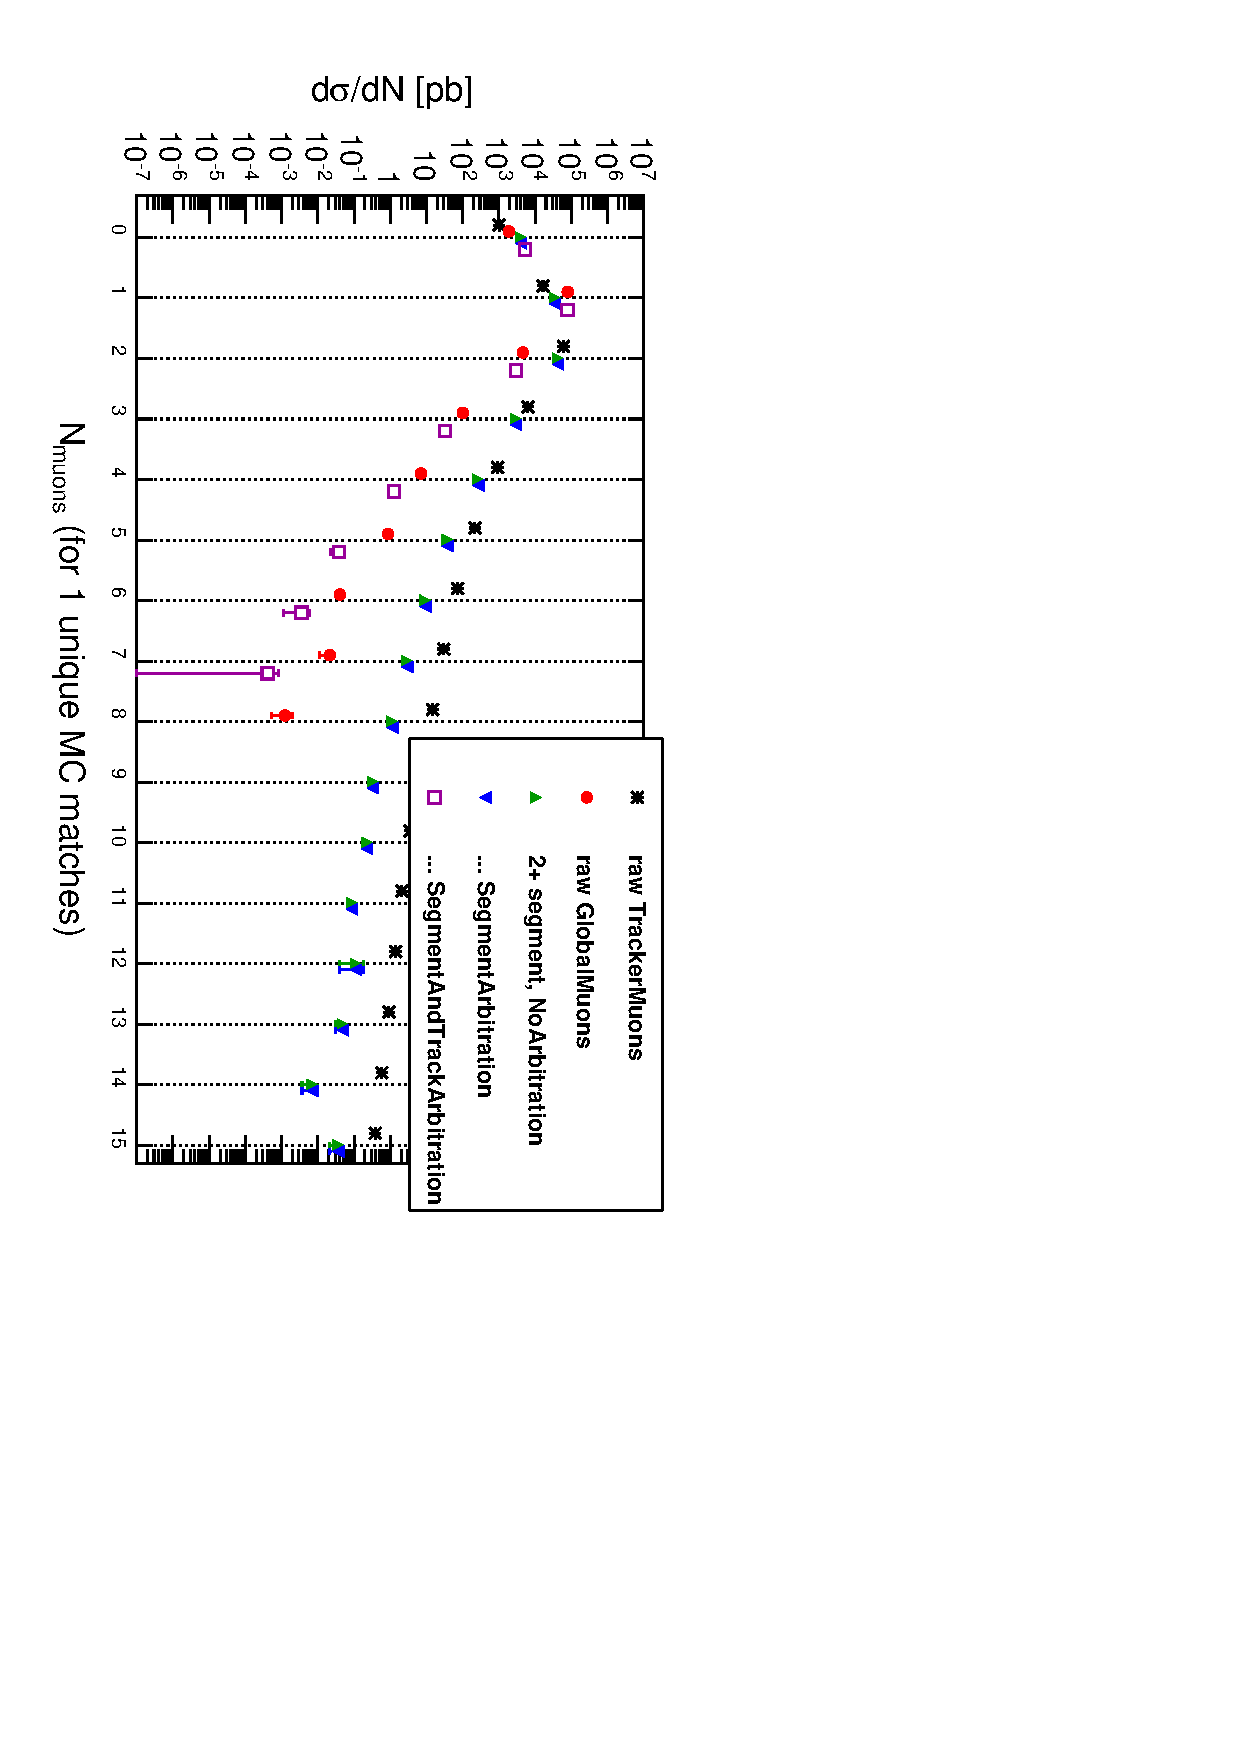
\includegraphics[height=0.5\linewidth, angle=90]{tracks_lastpage_1real.pdf}

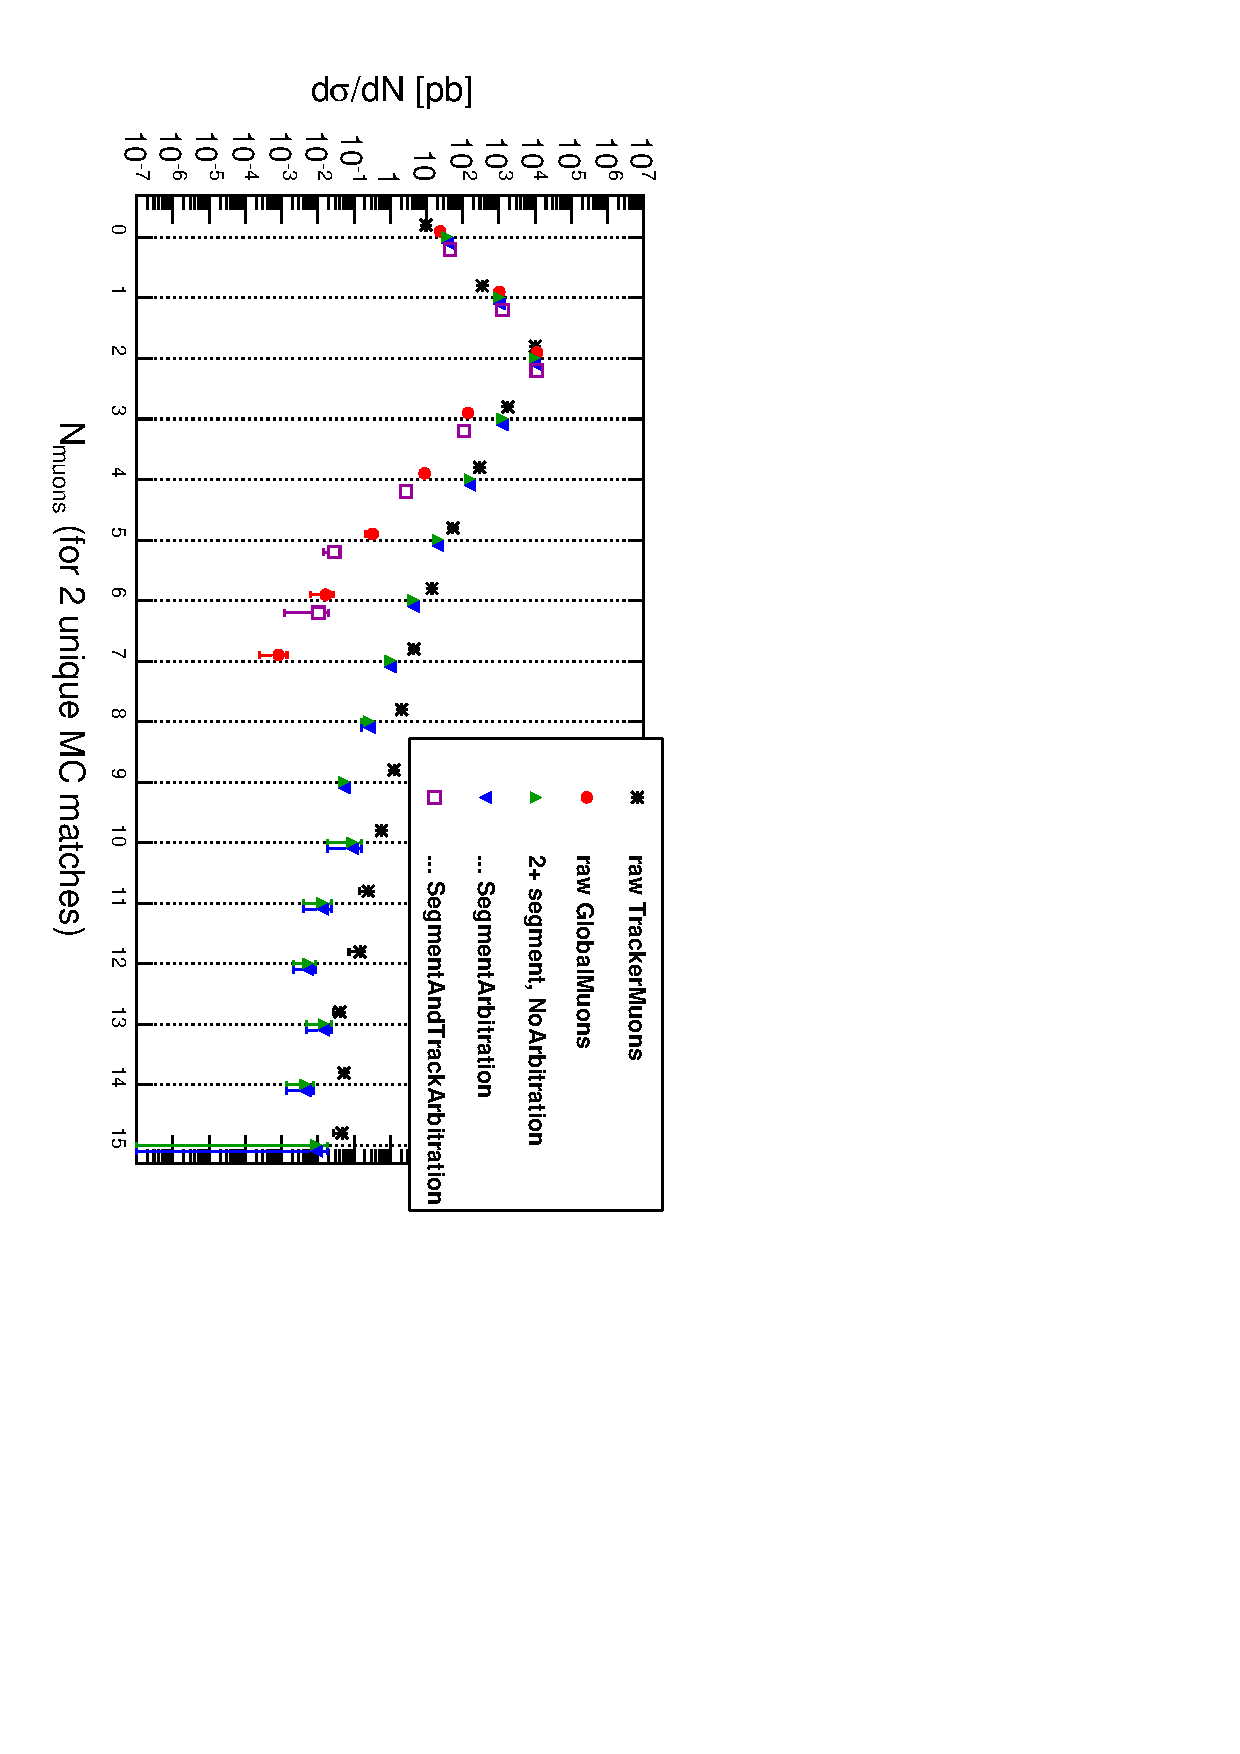
\includegraphics[height=0.5\linewidth, angle=90]{tracks_lastpage_2real.pdf}
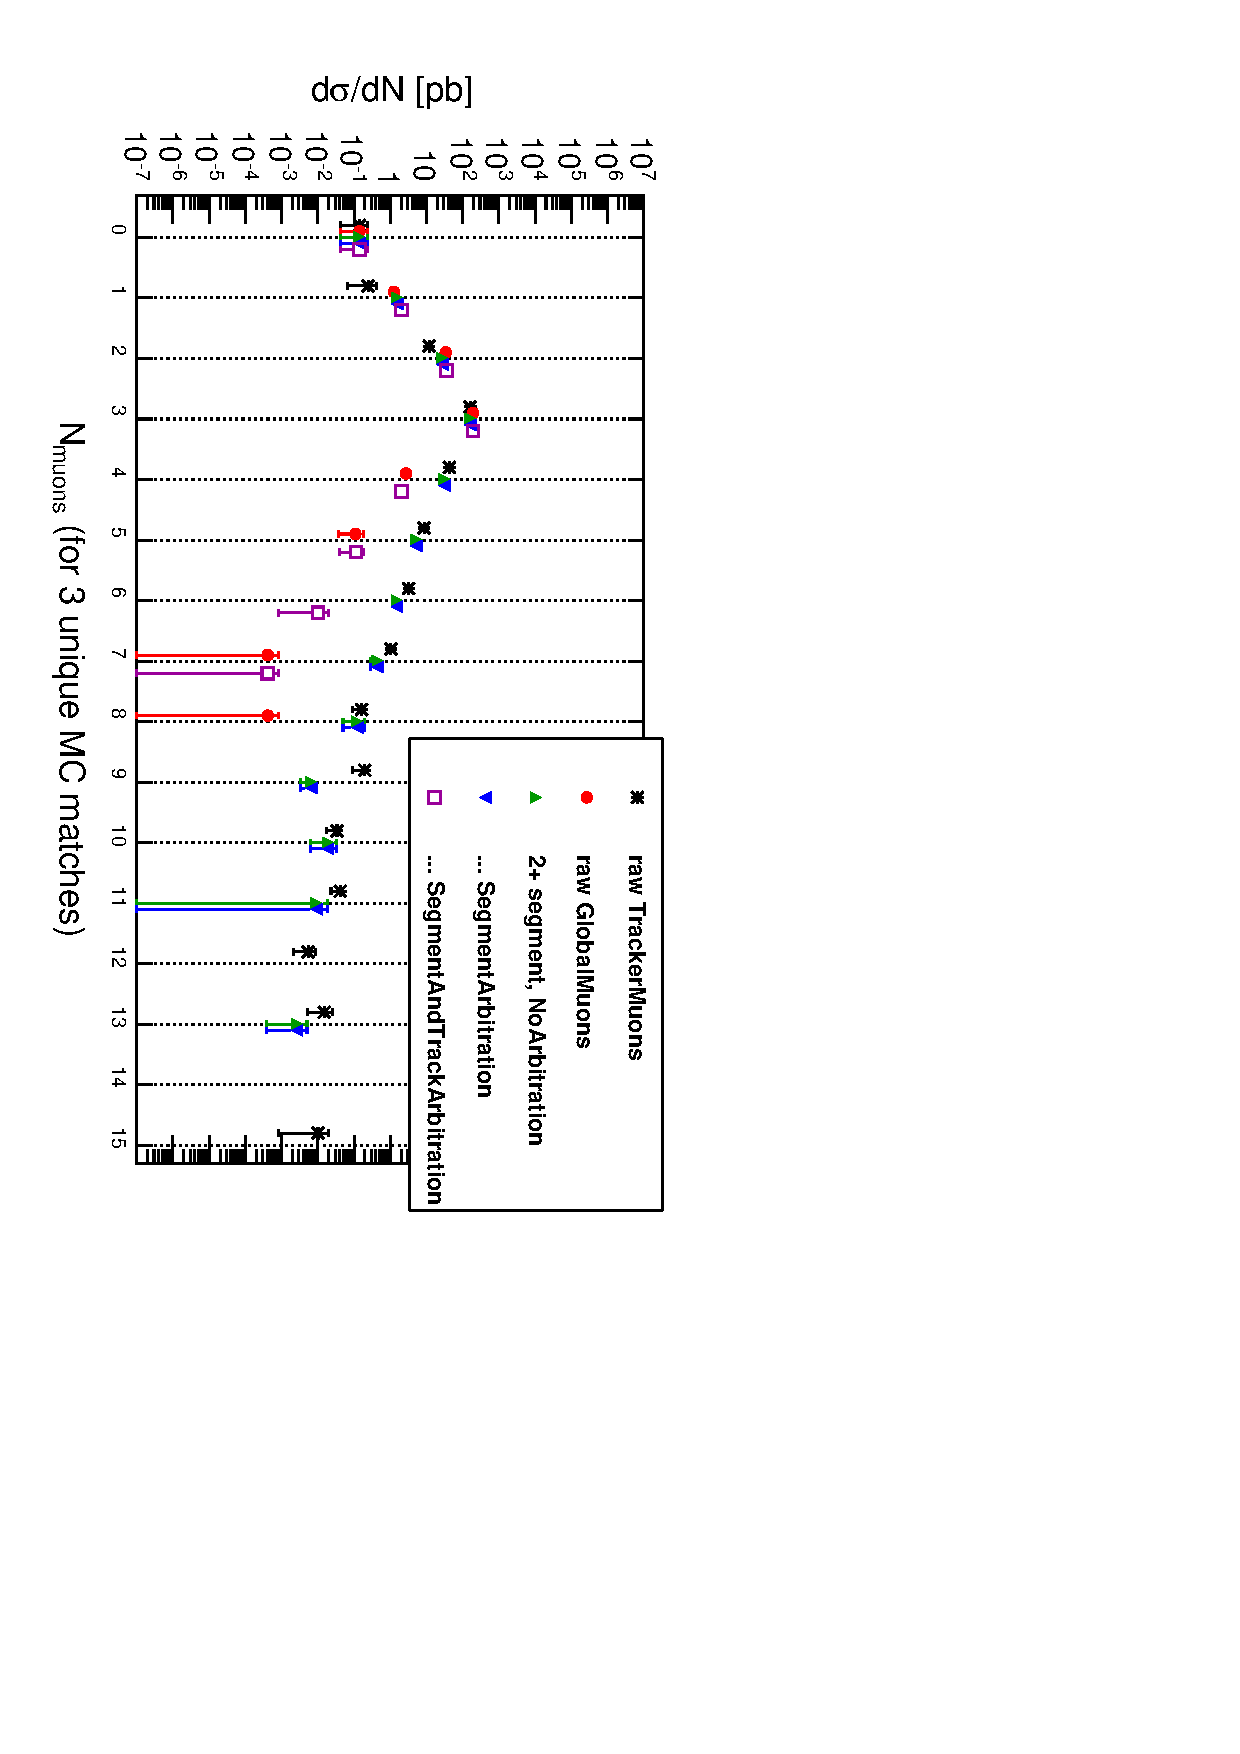
\includegraphics[height=0.5\linewidth, angle=90]{tracks_lastpage_3real.pdf}
\end{frame}

\begin{frame}
\frametitle{Quality-cut efficiency}

\begin{itemize}
\item TrackerMuon efficiency with $N_\s{segments} \ge 2$ (and other
  quality cuts) is still $\sim$95\% without a hard-to-model dip when
  pairs cross each other in the muon system
\end{itemize}

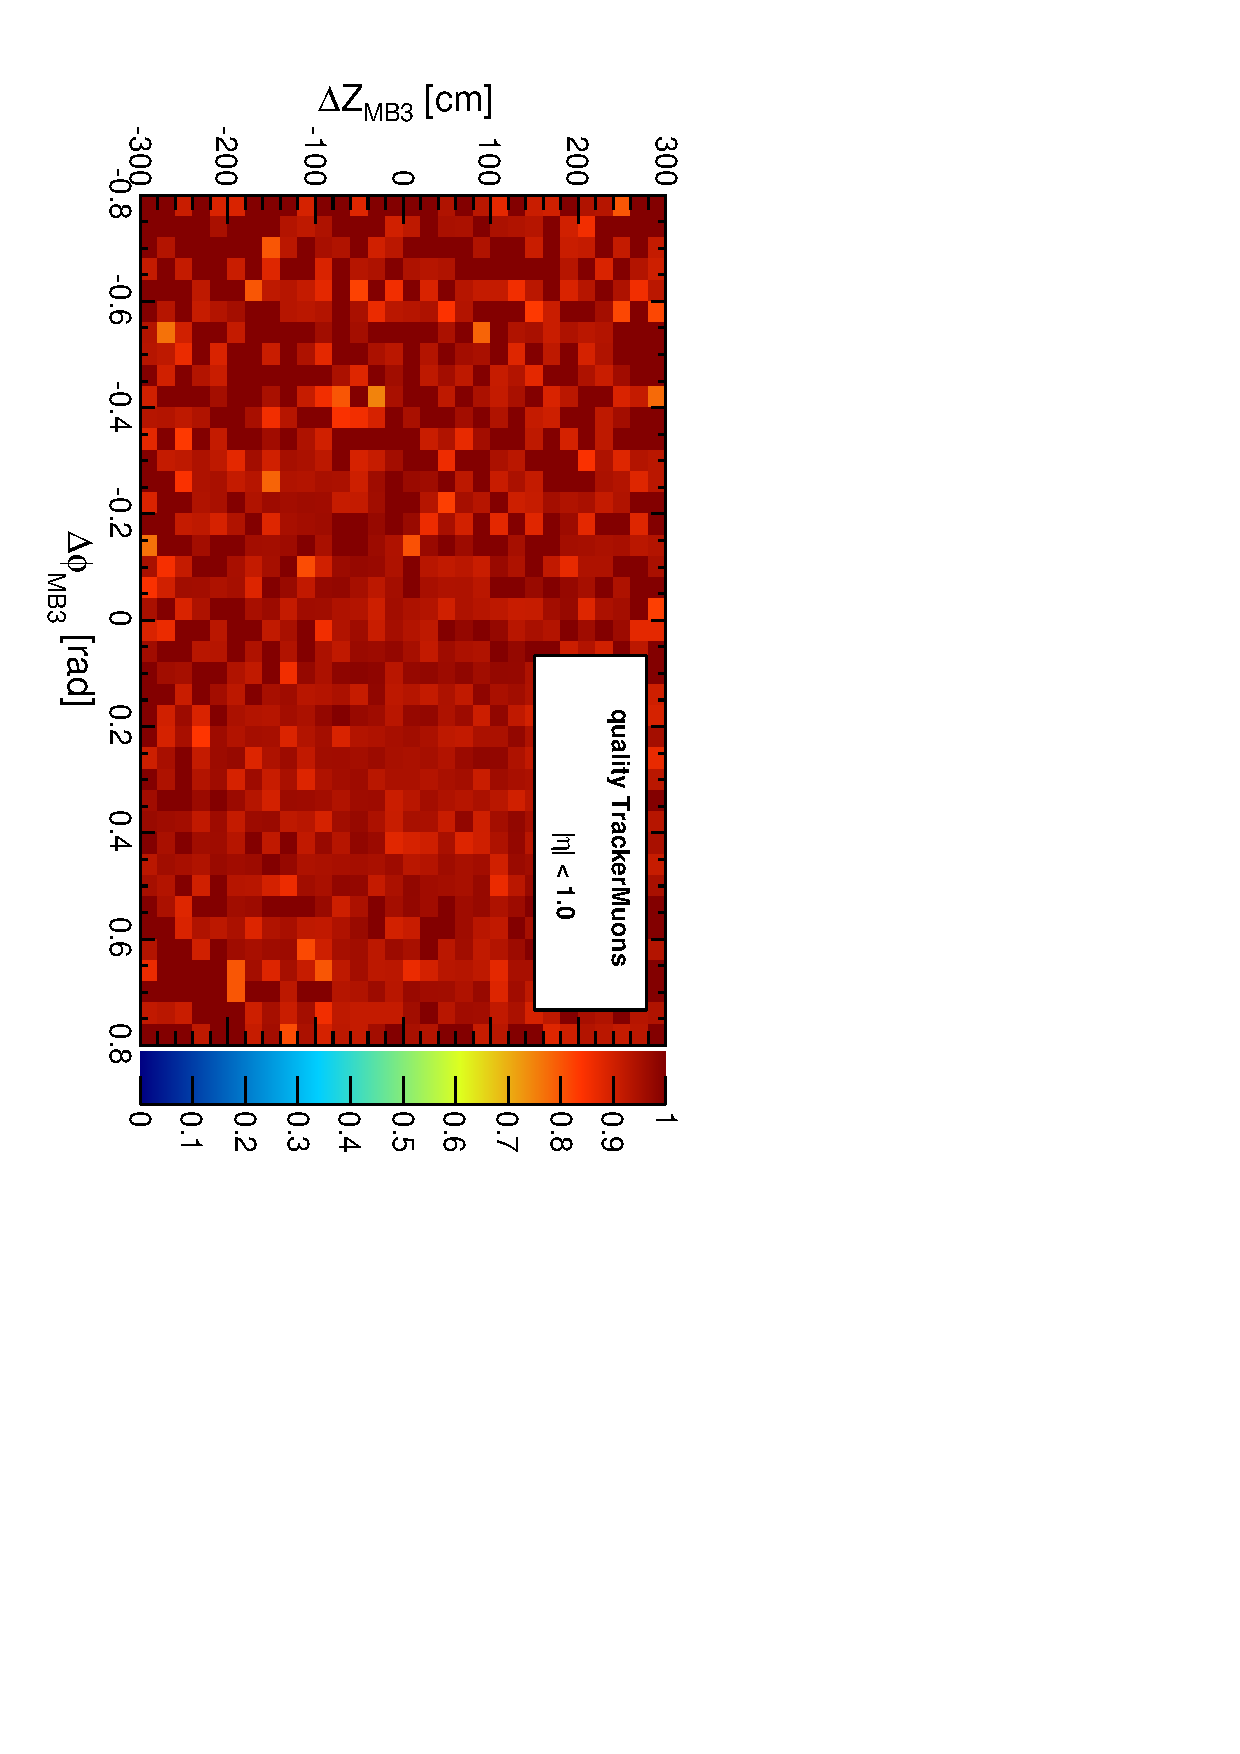
\includegraphics[height=0.5\linewidth, angle=90]{mb3_PlainTrackerMuon.pdf}
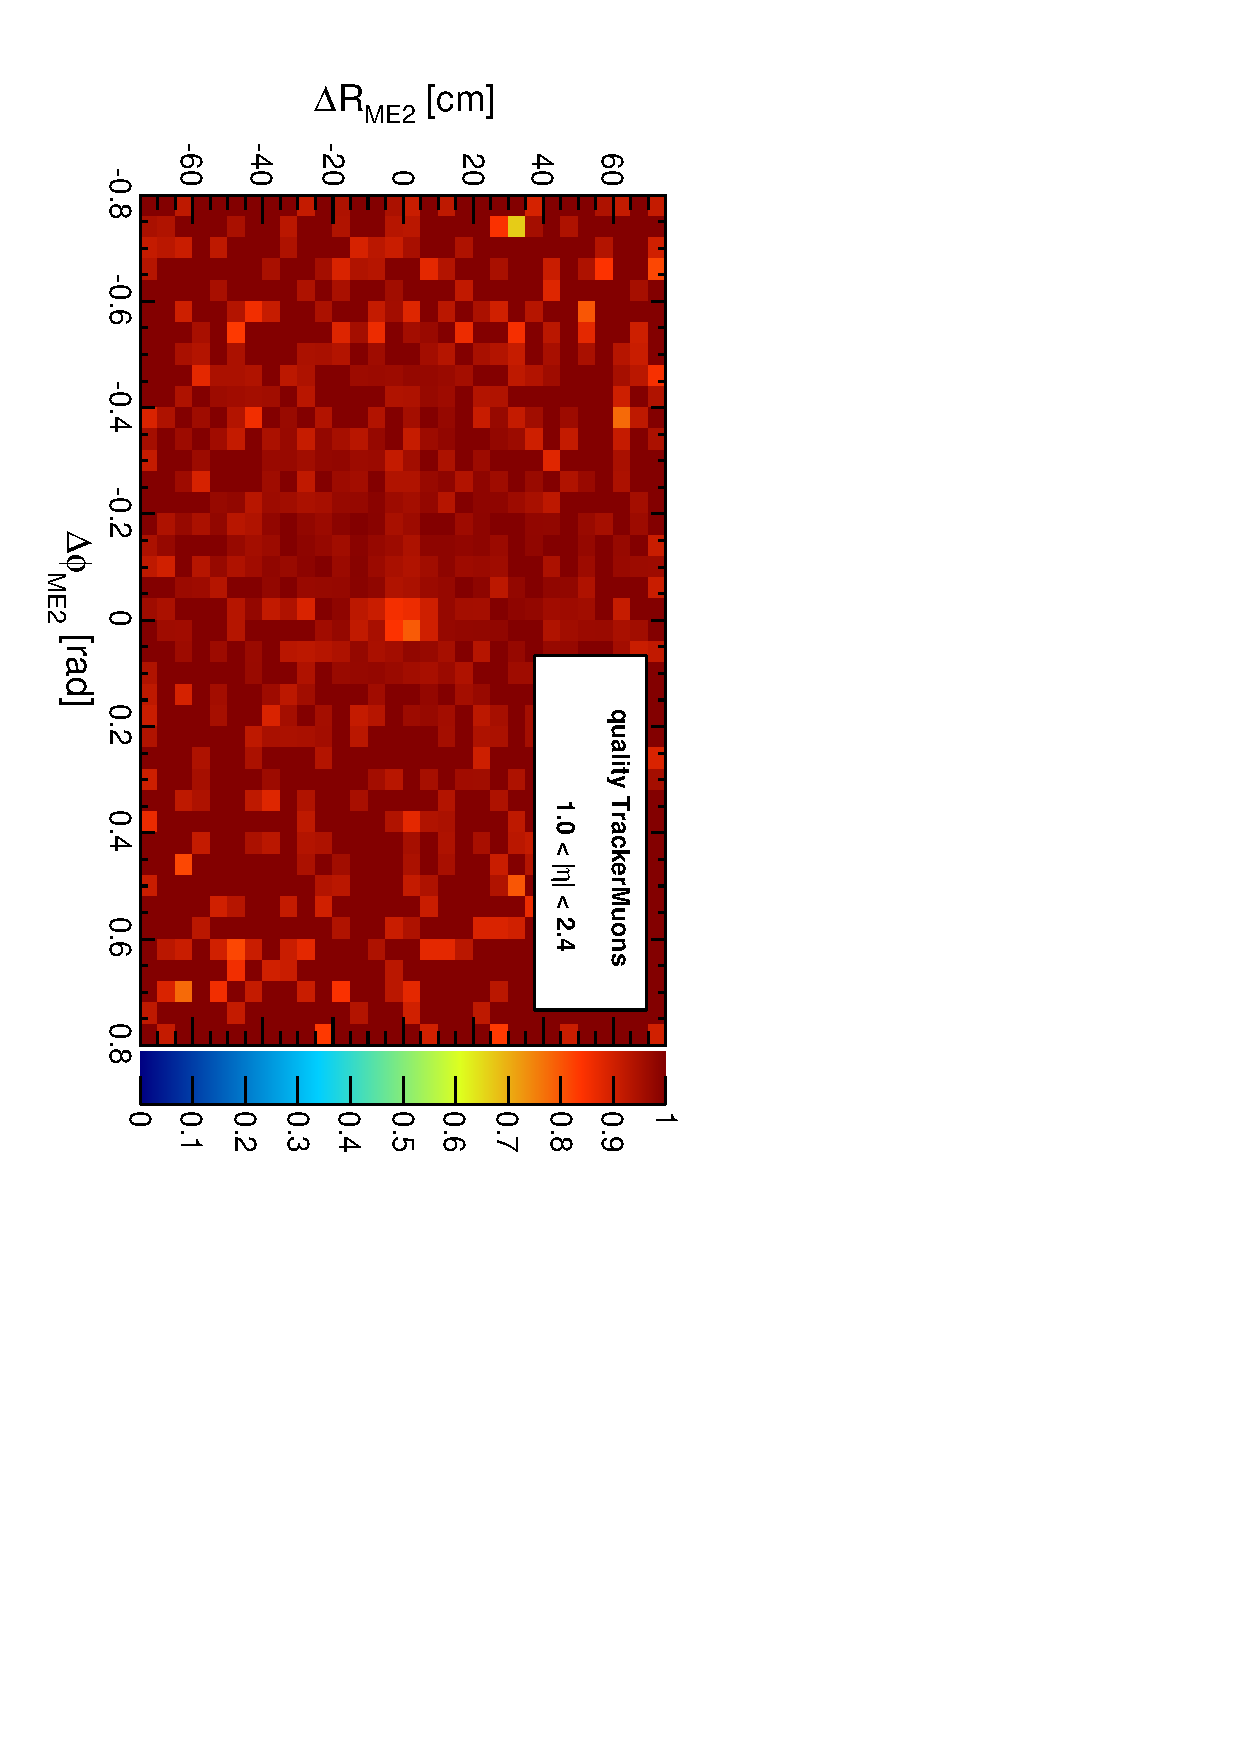
\includegraphics[height=0.5\linewidth, angle=90]{me2_PlainTrackerMuon.pdf}

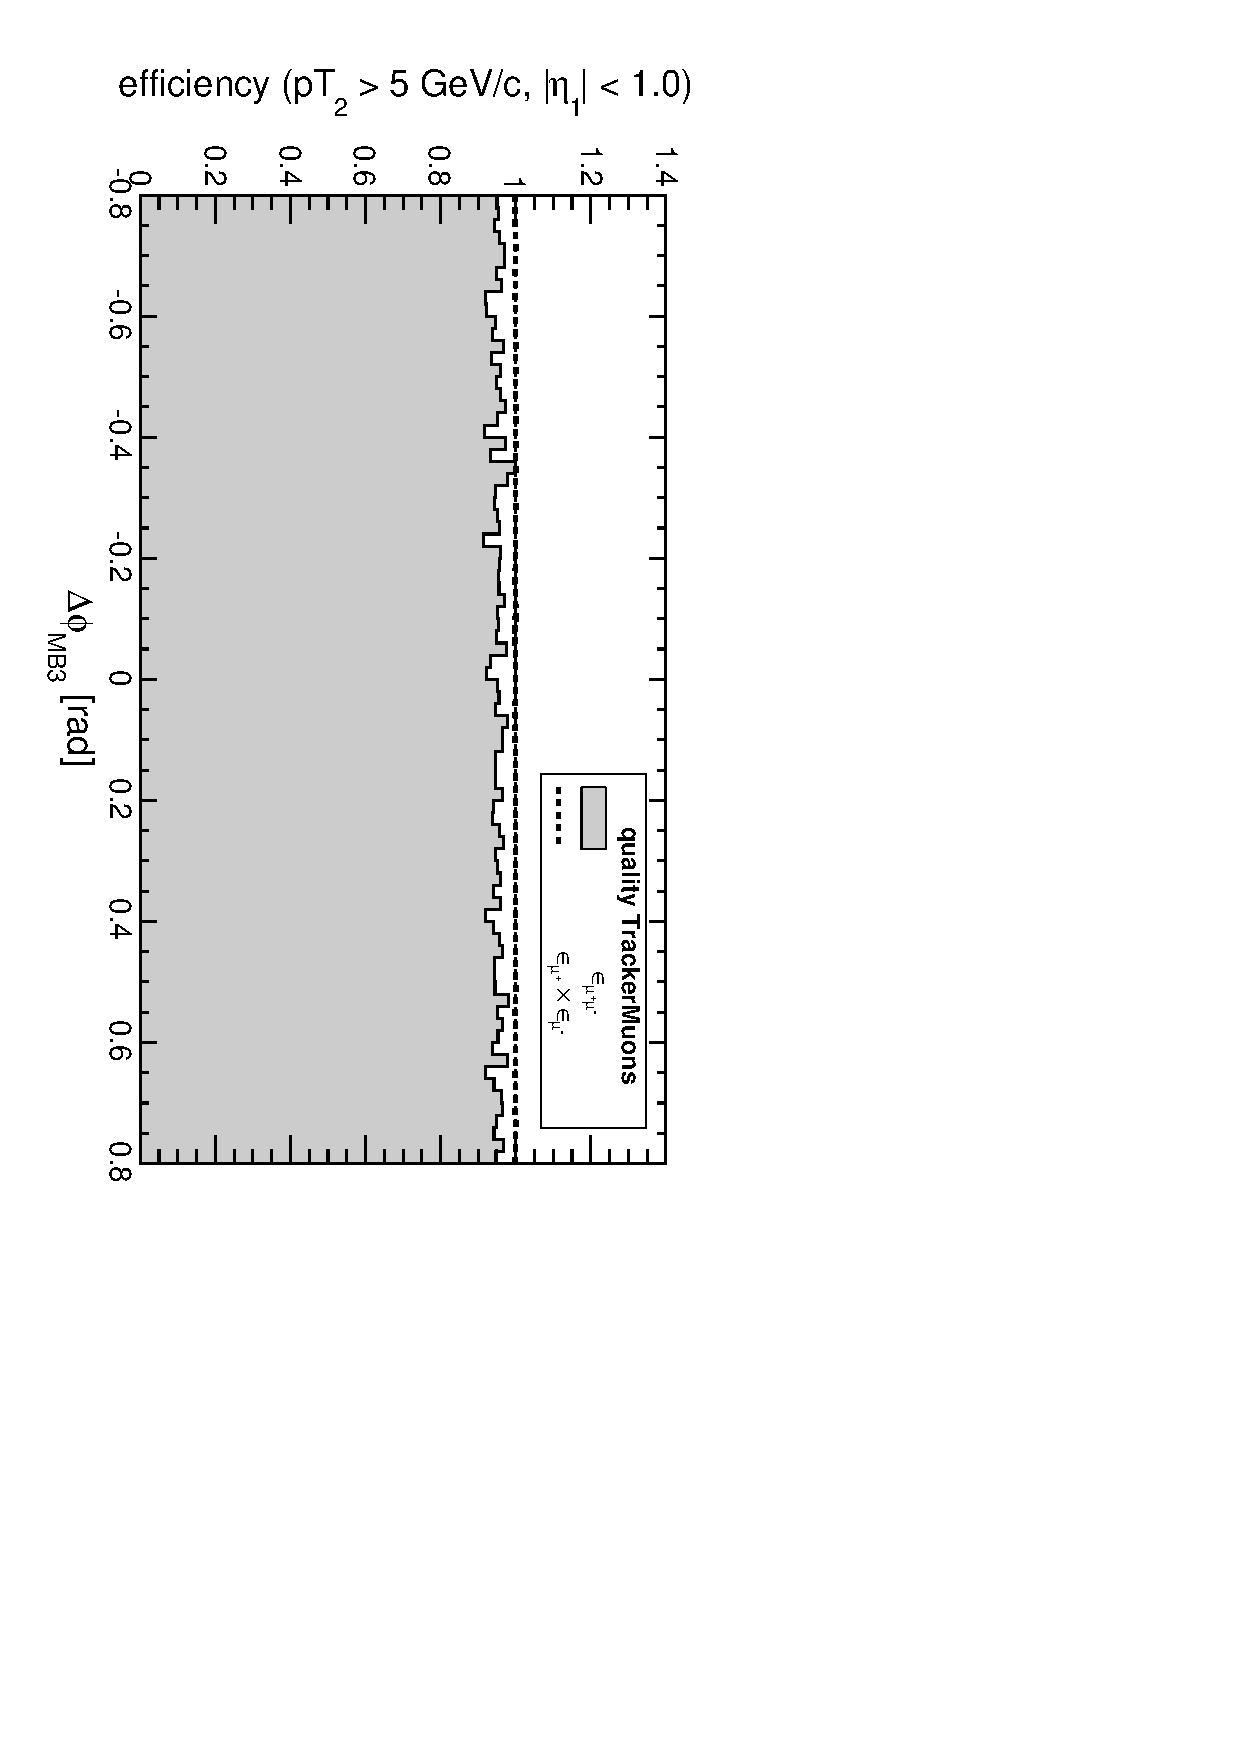
\includegraphics[height=0.5\linewidth, angle=90]{vsmb3dphi_PlainTrackerMuon.pdf}
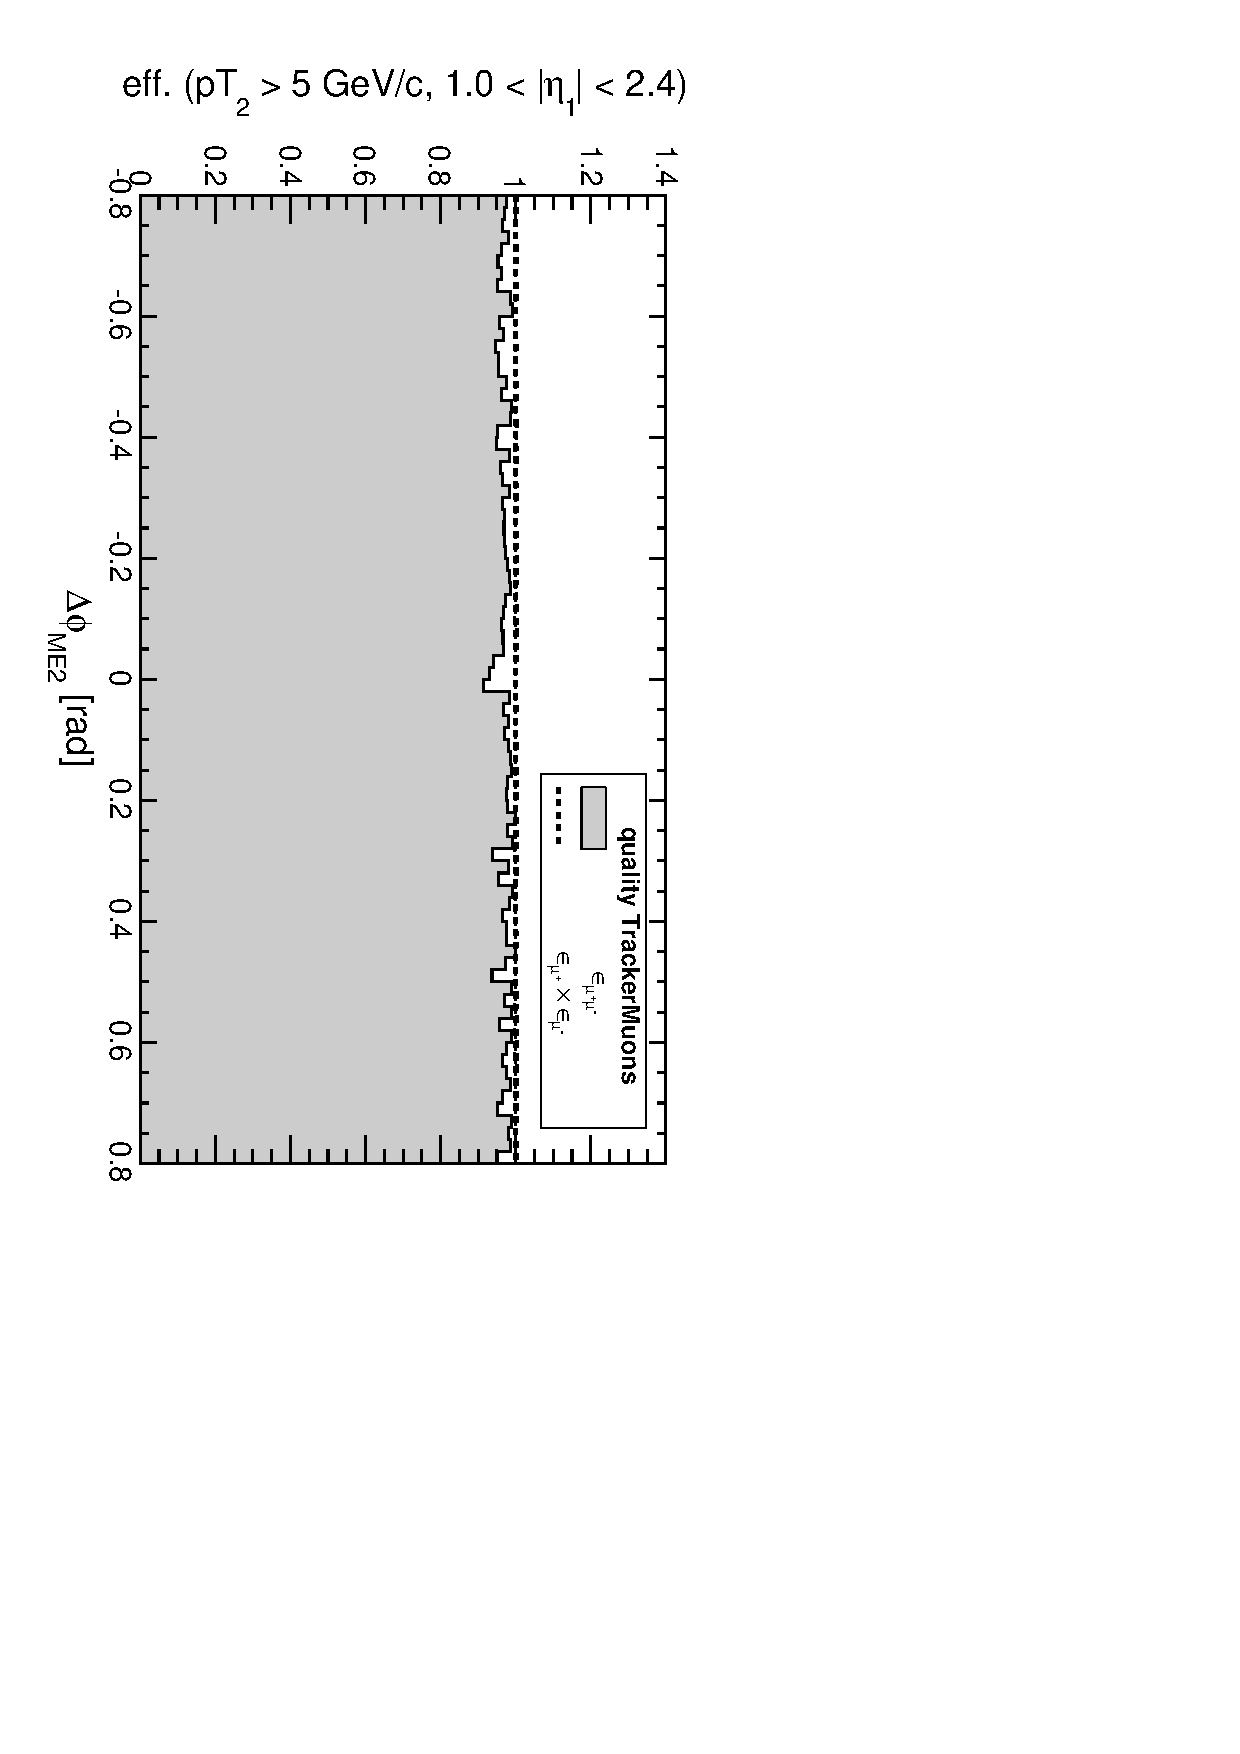
\includegraphics[height=0.5\linewidth, angle=90]{vsme2dphi_PlainTrackerMuon.pdf}
\end{frame}

\begin{frame}
\frametitle{Trigger efficiency}
\begin{itemize}
\item It may be a challenge to quantify our trigger efficiency

\item \textcolor{darkblue}{Issues in L1:}
\begin{itemize}
\item when multiple muons pass through the same chamber, only one may be read out
\item if an L1 muon is constructed from some $\mu^+$ segments and some $\mu^-$ segments, they may fail to be reconstructed as a single high-$p_T$ muon
\item this is not fully modeled in the L1 emulator!  (not for the CMSSW\_3\_6\_3 version that I'm using, anyway\ldots)
\end{itemize}
\item \textcolor{darkblue}{Issues in HLT:}
\begin{itemize}
\item uses StandAloneMuon reconstruction, with the inefficiencies already presented
\item only need to reconstruct one StandAloneMuon at HLT, not two, but reconstruction can still be confused by overlaps
\end{itemize}
\item Also, time-dependence as trigger conditions change
\end{itemize}
\end{frame}

\begin{frame}
\frametitle{QCD backgrounds: one $\mu$-group}

\begin{itemize}
\item The Standard Model has two clear signals in the one $\mu$-group
  channel: $J/\psi$ and $\phi(1020)$ (yellow)
\item $b \to c \to s$ with two semi-leptonic decays also correlates \mbox{muons (red)\hspace{-1 cm}}
\item<2> Only-one-muon (grey/blue) suppressed with
  opposite-sign grouping
\end{itemize}

\only<1>{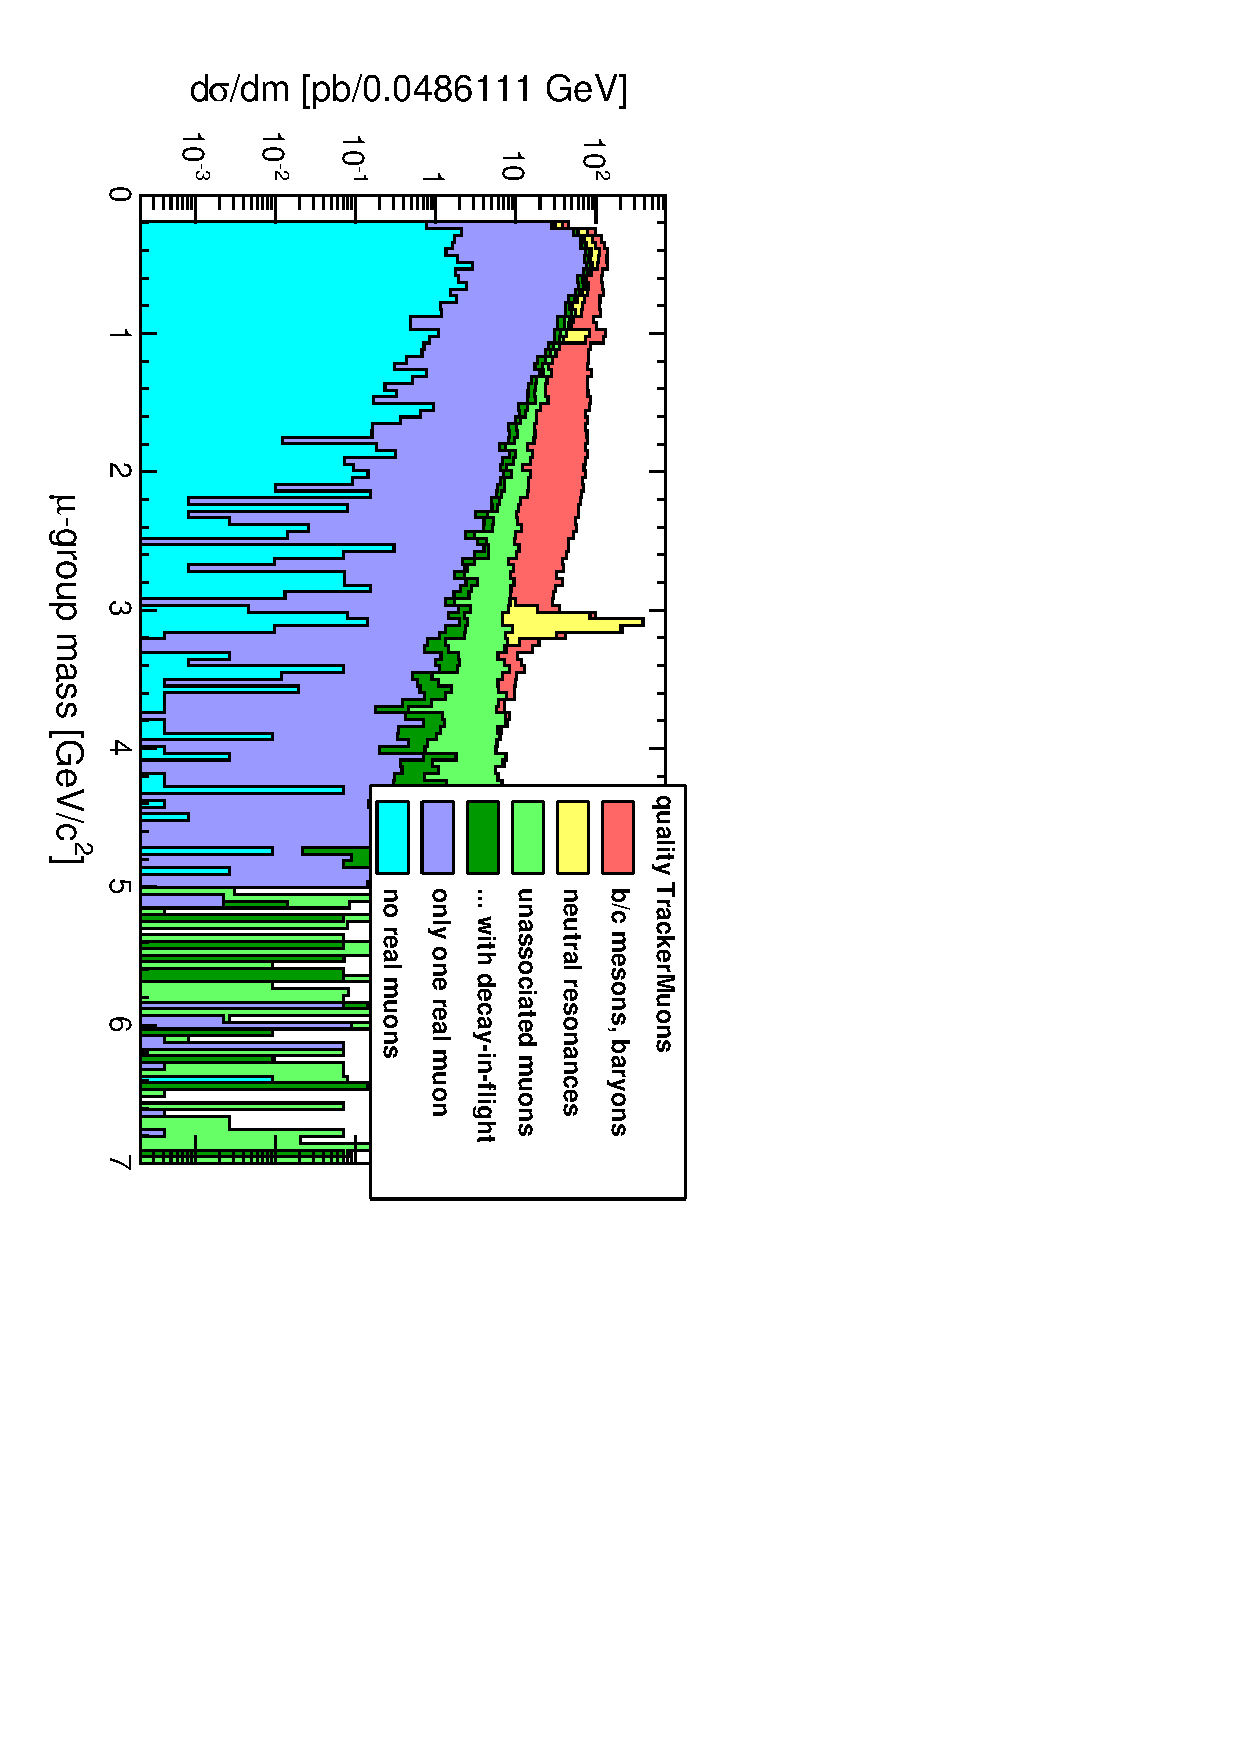
\includegraphics[height=0.5\linewidth, angle=90]{masslog_QualityTrackerMuonAny.pdf}
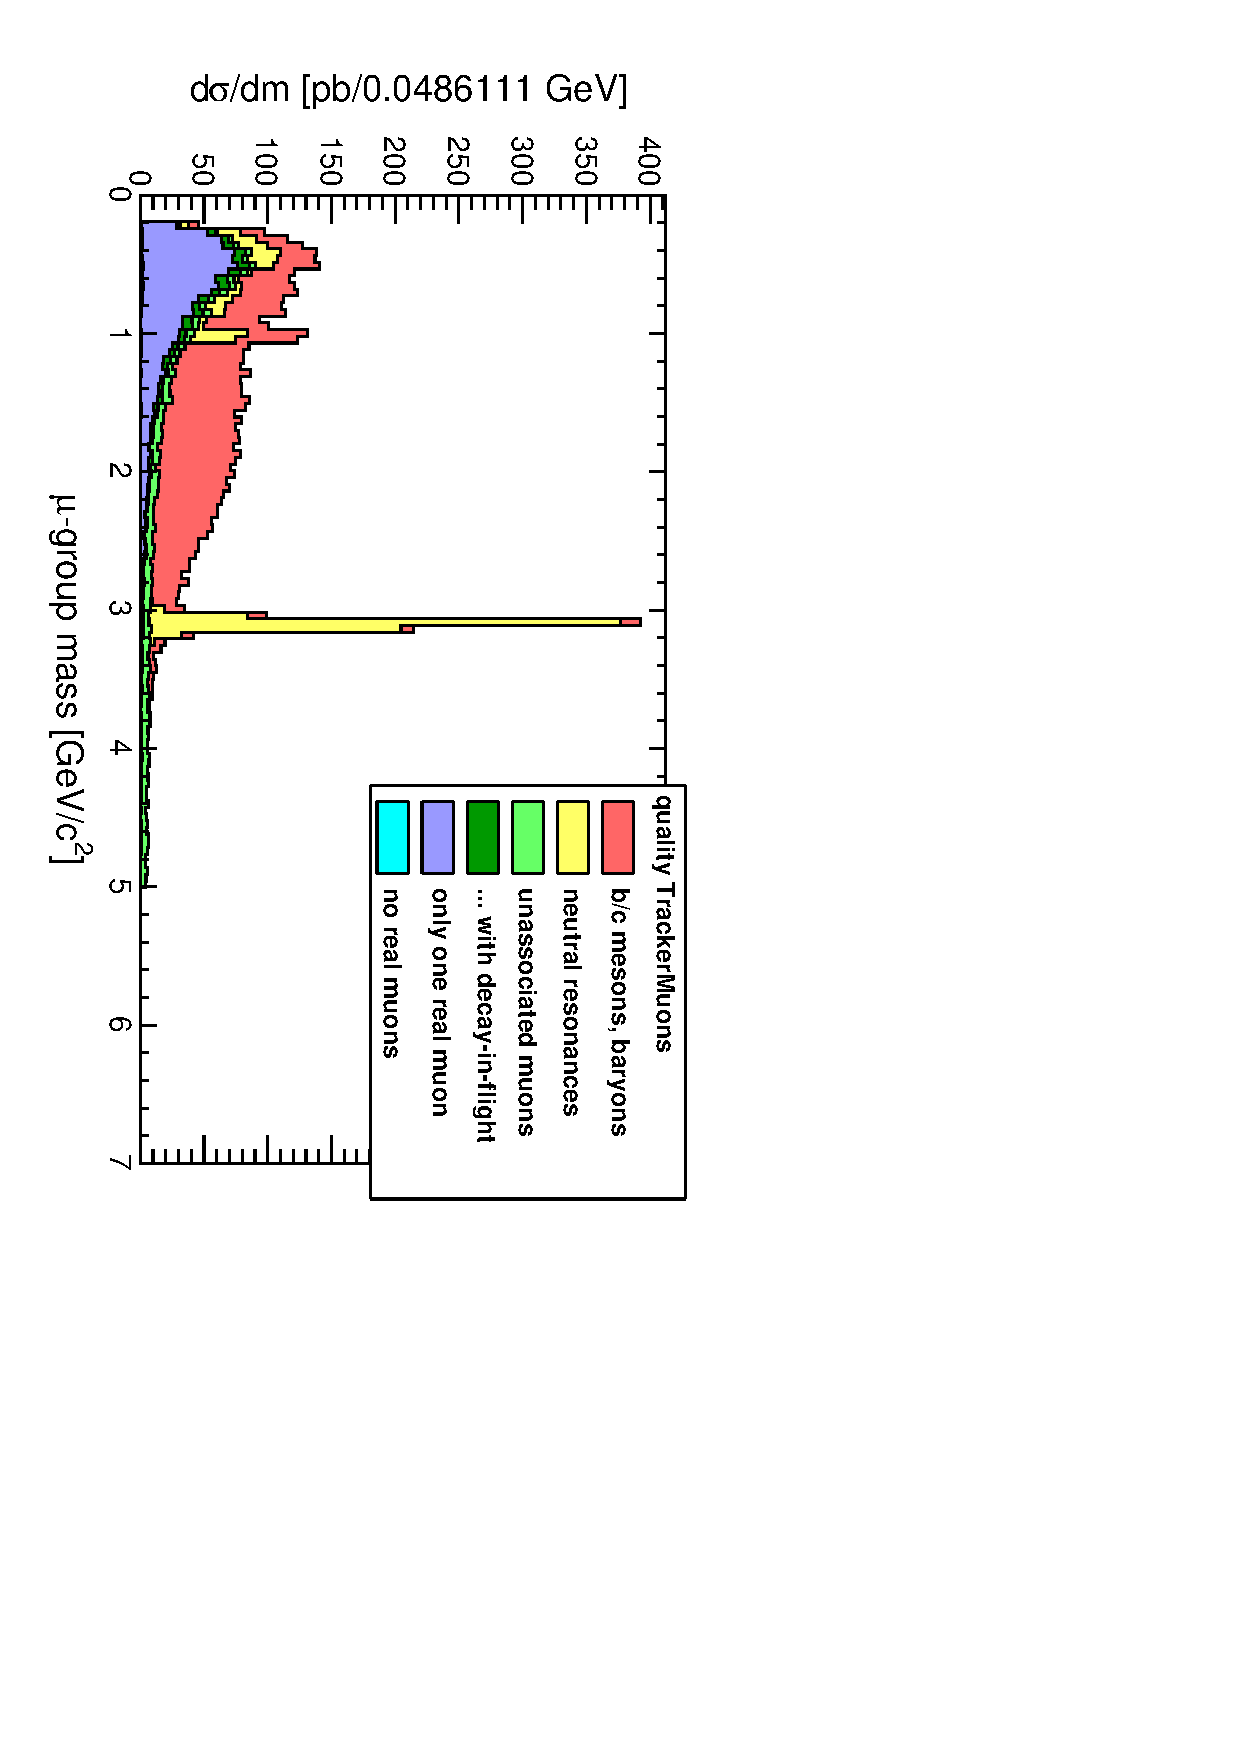
\includegraphics[height=0.5\linewidth, angle=90]{masslinear_QualityTrackerMuonAny.pdf}

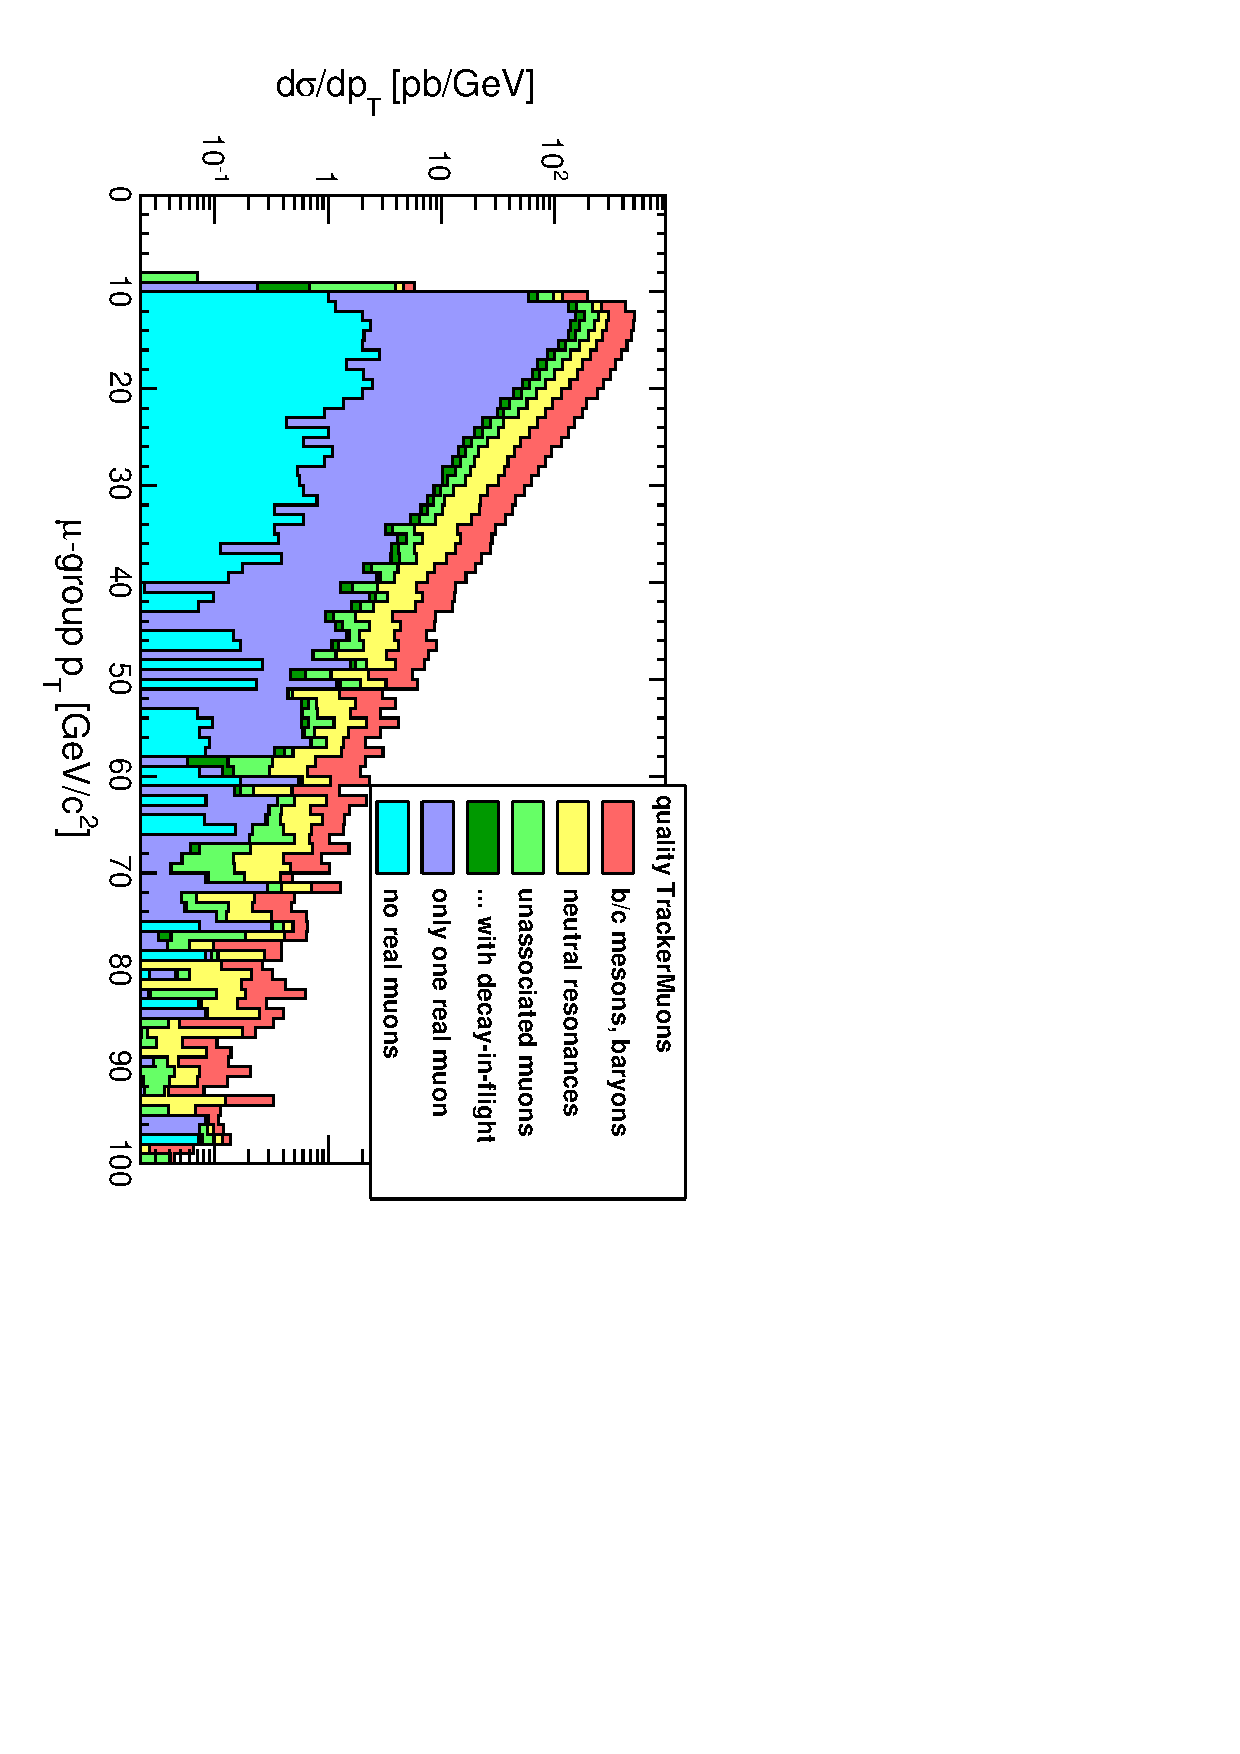
\includegraphics[height=0.5\linewidth, angle=90]{ptlog_QualityTrackerMuonAny.pdf}
\includegraphics[height=0.5\linewidth, angle=90]{ptlinear_QualityTrackerMuonAny.pdf}}
\only<2>{\includegraphics[height=0.5\linewidth, angle=90]{masslog_QualityTrackerMuonOpposite.pdf}
\includegraphics[height=0.5\linewidth, angle=90]{masslinear_QualityTrackerMuonOpposite.pdf}

\includegraphics[height=0.5\linewidth, angle=90]{ptlog_QualityTrackerMuonOpposite.pdf}
\includegraphics[height=0.5\linewidth, angle=90]{ptlinear_QualityTrackerMuonOpposite.pdf}}
\end{frame}

\begin{frame}
\frametitle{QCD backgrounds: one $\mu$-group}

\begin{itemize}
\item Just for fun: what it would look like without $N_\s{segments} \ge 2$ cut
\end{itemize}

\includegraphics[height=0.5\linewidth, angle=90]{masslog_PlainTrackerMuonAny.pdf}
\includegraphics[height=0.5\linewidth, angle=90]{masslinear_PlainTrackerMuonAny.pdf}

\includegraphics[height=0.5\linewidth, angle=90]{ptlog_PlainTrackerMuonAny.pdf}
\includegraphics[height=0.5\linewidth, angle=90]{ptlinear_PlainTrackerMuonAny.pdf}
\end{frame}

\begin{frame}
\frametitle{Multiple $\mu$-groups}

\begin{itemize}
\item Asking for a second $\mu$-group reduces the QCD backgrounds to 1~pb
\item Many of the models we've looked at have $\sim$pb cross-sections or at least limits can be set with 1--100~pb$^{-1}$
\item Since we're looking for new resonances, we get more sensitivity
  by searching for peaks: the QCD backgrounds are roughly flat in mass
\end{itemize}

\includegraphics[height=4 cm]{groups_QualityTrackerMuonAny.pdf}
\includegraphics[width=4 cm, angle=90]{m12m34bypt_QualityTrackerMuonAny.pdf}
\end{frame}

\begin{frame}
\frametitle{Signals: mass peaks}

\begin{columns}
\column{0.5\linewidth}
Pair-pair $\mu$ gun with both pairs having the same mass

\includegraphics[height=\linewidth, angle=90]{m12m34.pdf}

\column{0.5\linewidth}
NMSSM Higgs with $h \to aa \to 4\mu$ ($m_h = 100$, $m_a = 2$~GeV/$c^2$)

\only<1>{\includegraphics[height=\linewidth, angle=90]{m12m34_bypt_NMSSM_pileup_QualityTrackerMuonAny.pdf}}
\only<2>{\includegraphics[height=\linewidth, angle=90]{m12m34_bypt_NMSSM_pileup_QualityTrackerMuonAny_lego.pdf}}
\end{columns}

\vspace{0.25 cm}
\begin{columns}
\column{0.5\linewidth}
Extra-$\mathcal{U}(1)$ dark matter model with $\gamma_\s{dark} \to
\mu^+\mu^-$, $m_\gamma = 1$~GeV/$c^2$

\only<1>{\includegraphics[height=\linewidth, angle=90]{m12m34_bypt_ExtraU1_pileup_QualityTrackerMuonAny.pdf}}
\only<2>{\includegraphics[height=\linewidth, angle=90]{m12m34_bypt_ExtraU1_pileup_QualityTrackerMuonAny_lego.pdf}}

\column{0.5\linewidth}
Same with $h_\s{dark} \to \gamma_\s{dark} \gamma_\s{dark}$, $m_h
= 3$~GeV/$c^2$ and $m_\gamma = 1$~GeV/$c^2$

\only<1>{\includegraphics[height=\linewidth, angle=90]{m12m34_bypt_ExtraU1higgs_pileup_QualityTrackerMuonAny.pdf}}
\only<2>{\includegraphics[height=\linewidth, angle=90]{m12m34_bypt_ExtraU1higgs_pileup_QualityTrackerMuonAny_lego.pdf}}
\end{columns}
\end{frame}

\begin{frame}
\frametitle{Isolation variables}
\begin{center}
\includegraphics[width=0.7\linewidth]{isolation.pdf}
\end{center}
\begin{itemize}
\item $\sum |p_T|$ in a cone of $\Delta R < 0.3$
\item Vertical axis only applies to backgrounds (the rest are arbitrarily normalized)
\end{itemize}
\begin{center}
\includegraphics[height=0.8\linewidth, angle=90]{tkisolation_QualityTrackerMuonAny_all.pdf}
\end{center}
\end{frame}

\begin{frame}
\frametitle{Displaced vertices}
\begin{itemize}
\item To have avoided detection so far, dark-sector boson must be weakly coupled to Standard Model
\item In an extreme case, it could decay far from beamline
\item Displaced-dimuon efficiency {\scriptsize (denominator: all $pT_2 > 5$~GeV/$c$, $|\eta_1| < 2.4$, mass $<$ 5~GeV/$c^2$; numerator: found trigger or muon-groups, respectively)}
\begin{itemize}
\item HLT muon trigger depends on StandAloneMuon with beamline-constraint
\item special 7-iteration tracking (for $\gamma$ conversions; light green) doesn't help much in its out-of-the-box configuration
\end{itemize}
\end{itemize}

\includegraphics[width=3.5 cm, angle=90]{dispvert.pdf} \hfill \includegraphics[height=3.5 cm]{leptjets1e.pdf}
\end{frame}

\begin{frame}
\frametitle{Displaced vertices}
\begin{itemize}
\item Quality cuts seem to be cutting both signal and background:
  something should possibly be loosened for the displaced-vertex case
\item Left: QCD background effective cross-section; right: \mbox{signal efficiency\hspace{-1 cm}}
\item Top: no quality cuts; bottom: with quality cuts
\item<2> Same for GlobalMuons \mbox{(uncut GlobalMuon backgrounds are 1~pb/cm)\hspace{-1 cm}}
\end{itemize}

\begin{center}
\only<1>{\includegraphics[height=0.45\linewidth, angle=90]{dispvert_PlainTrackerMuonAny.pdf}
\includegraphics[height=0.45\linewidth, angle=90]{dispvert_eff_PlainTrackerMuonAny.pdf}

\includegraphics[height=0.45\linewidth, angle=90]{dispvert_QualityTrackerMuonAny.pdf}
\includegraphics[height=0.45\linewidth, angle=90]{dispvert_eff_QualityTrackerMuonAny.pdf}}
\only<2>{\includegraphics[height=0.45\linewidth, angle=90]{dispvert_PlainGlobalMuonAny.pdf}
\includegraphics[height=0.45\linewidth, angle=90]{dispvert_eff_PlainGlobalMuonAny.pdf}

\includegraphics[height=0.45\linewidth, angle=90]{dispvert_QualityGlobalMuonAny.pdf}
\includegraphics[height=0.45\linewidth, angle=90]{dispvert_eff_QualityGlobalMuonAny.pdf}}
\end{center}
\end{frame}

%% \begin{frame}
%% \frametitle{Outline}
%% \begin{itemize}\setlength{\itemsep}{0.75 cm}
%% \item 
%% \end{itemize}
%% %% \hspace{-0.83 cm} \textcolor{darkblue}{\Large Outline2}
%% \end{frame}

%% \section*{First section}
%% \begin{frame}
%% \begin{center}
%% \Huge \textcolor{blue}{First section}
%% \end{center}
%% \end{frame}

\begin{frame}
\frametitle{Conclusions}
\begin{itemize}\setlength{\itemsep}{0.2 cm}
\item Muon-grouping algorithm designed to find low-mass resonances, no
  matter how boosted or how many are in the event
\item StandAlone/GlobalMuon inefficiencies traced to overlapping
  trajectories in the endcap, still not clear in the barrel
\item TrackerMuons have high, uniform efficiency, and large
  backgrounds can be suppressed by requiring $N_\s{segments} \ge 2$
  with track-and-segment arbitration
\item Understanding the exact trigger efficiency will be challenging
\item Two $\mu$-group QCD backgrounds are 1~pb and $\sim$flat in mass
\item Displaced vertex case has not been fully optimized
\end{itemize}
\label{numpages}
\end{frame}

\end{document}
